\chapter{贫 血}

贫血是指外周血中单位体积内血红蛋白(Hb)浓度、红细胞(RBC)计数和(或)血细胞比容(HCT)低于相同年龄、性别和地区的正常标准。一般认为,成年男性Hb<120g/L,成年女性Hb<110g/L,孕妇<100g/L;成年男性RBC<4.5×10\textsuperscript{12}
/L及(或)HCT<42\%,成年女性RBC<4.0×10\textsuperscript{12}
/L及(或)HCT<37\%可以诊断为贫血。其中,以Hb浓度低于正常最为重要。贫血严重程度划分标准为:Hb>90g/L为轻度,Hb
60~90g/L为中度,Hb
30~60g/L为重度,Hb<30g/L为极重度。贫血仅是一个症状,而非一种疾病。引起贫血的原因很多,临床上贫血的诊断第一步骤是明确贫血存在与否,贫血的程度与类型;第二步骤是查明贫血的原因或引起贫血的原发病。贫血分类方法很多,可根据其发生的病理生理或红细胞形态进行分类,但这两种分类法仍有一定缺陷。

按贫血发生的病理生理,贫血可分为三大类(表\ref{tab33-1})。

(1)失血后贫血:由于外出血或内出血所致的血液丧失。

(2)红细胞破坏过多:由于先天性遗传性因素或后天获得性因素所致。后者又分为免疫性与非免疫性溶血性贫血两类。

(3)红细胞生成减少:因造血营养物质的缺乏,或造血细胞、组织结构和功能的不正常,以致红细胞与血红蛋白生成障碍。

根据红细胞平均容积(MCV)和红细胞平均血红蛋白浓度(MCHC)进行形态学的分类(表\ref{tab33-2}),可将贫血区分为下列三种类型:

(1)大细胞性贫血:红细胞平均容积增大,红细胞平均血红蛋白浓度正常。如巨幼细胞性贫血、溶血性贫血、骨髓增生异常综合征、肝病及甲状腺功能减退等。

(2)正细胞性贫血:红细胞平均容积和红细胞平均血红蛋白浓度均正常。属于此类贫血的主要有急性失血后贫血、溶血性贫血、再生障碍性贫血、脾功能亢进、慢性肾衰竭引起的贫血等。

(3)小细胞低色素性贫血:红细胞平均容积减小,红细胞平均血红蛋白浓度明显减少。如缺铁性贫血、珠蛋白生成障碍性贫血、慢性病性贫血及铁粒幼细胞性贫血等。

病因及发病机制分类法对贫血的病因及发病机制有所说明,利于对贫血的诊断和治疗,但病因分类也有不足之处,一个由多种因素所致的贫血,其发病原因往往不单纯为一种,两种或两种以上的发病原因也非罕见。如对慢性疾病所致的贫血就无法进行简单的归类;慢性失血性贫血同时又是一种缺铁性贫血等。

\begin{table}[htbp]
\centering
\caption{贫血疾病的分类}
\label{tab33-1}
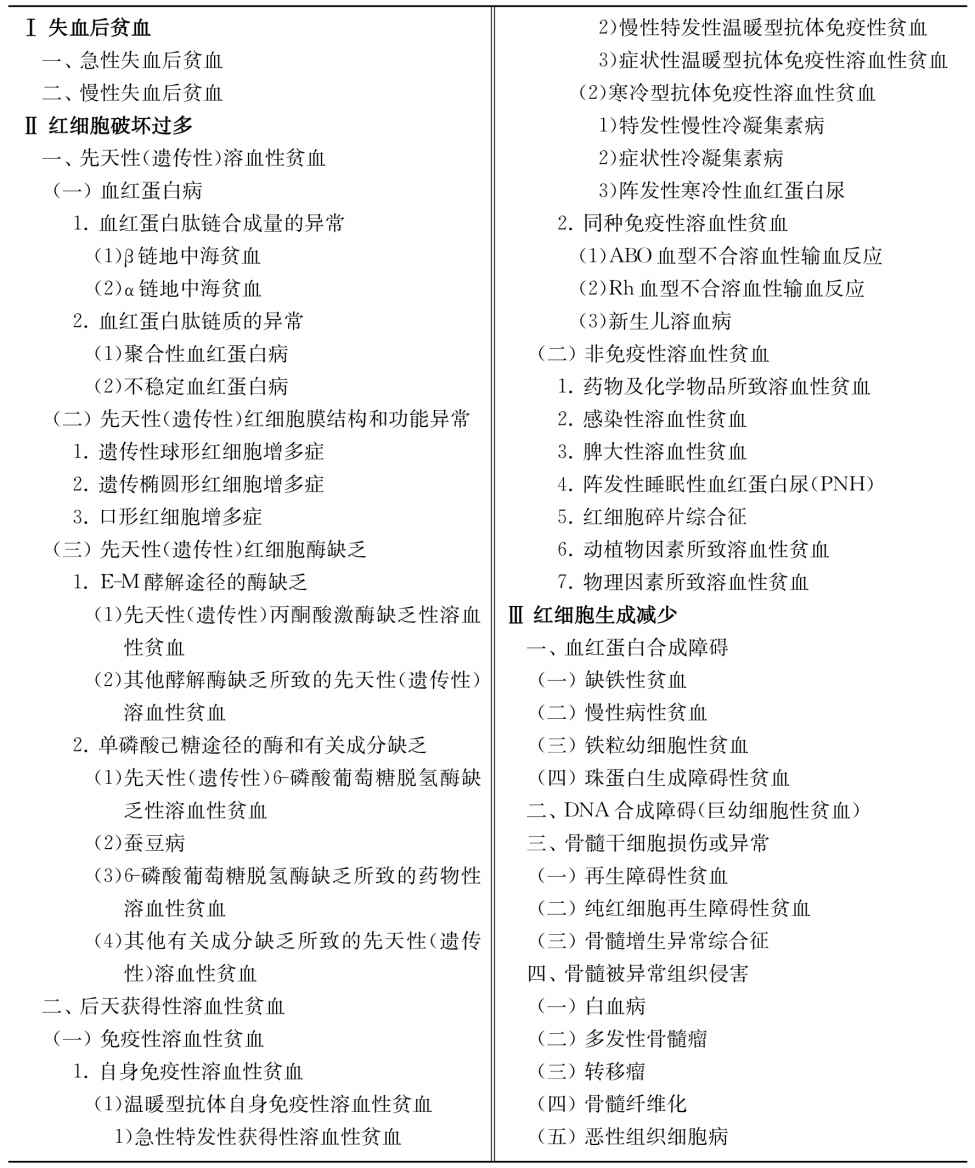
\includegraphics[width=5.91667in,height=7.08333in]{./images/Image00163.jpg}
\end{table}

\begin{table}[htbp]
\centering
\caption{贫血的细胞形态学分类}
\label{tab33-2}
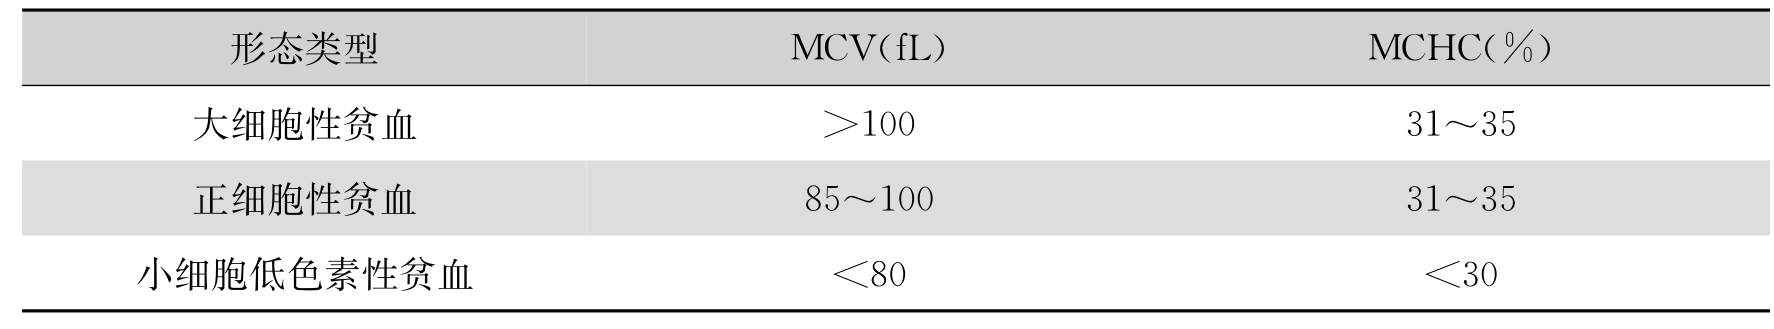
\includegraphics[width=5.90625in,height=1.08333in]{./images/Image00164.jpg}
\end{table}

形态学分类可提供对贫血的诊断与鉴别诊断的线索,但测定MCV和MCHC要求十分准确,否则可得出错误的结论,而且形态学分类过于简单机械,有些情况不能单纯依靠形态学的分类进行诊断及鉴别诊断。例如巨幼细胞性贫血伴有缺铁性贫血即所谓“混合性”贫血时,红细胞平均容积可以正常。如溶血性贫血可为大或正细胞性贫血,但当长期反复发作血红蛋白尿时,也可能因缺铁出现小细胞性贫血。一般认为,贫血的分类应一方面根据形态学分类而同时又紧密地结合病因学分类来考虑,这样才能对贫血作出较准确而全面的诊断。

贫血首先应与“生理性贫血”或“假性贫血”相区别。“生理性贫血”可见于妊娠等,“假性贫血”出现在低白蛋白血症、充血性心力衰竭、全身性水肿等。“生理性贫血”或“假性贫血”时总的血红蛋白量和总的红细胞数并无减少,其所以表现出贫血,主要是由于血容量增加,血液稀释致血红蛋白量和红细胞数偏低。

贫血的诊断确定以后,应作出贫血病因或引起贫血的原发病的诊断。贫血的病因有时很明显,但有时很隐蔽。诊断贫血首先必须深入了解病史、全面细致的体格检查、做好一般的实验室检查,从而作出初步的诊断,然后再有目的地进行某些必要的、复杂的特殊检查,最后根据所有的资料进行综合分析,得出正确结论。

\section{(一)病史和体征}

病史和体征在贫血病因诊断上占重要地位,但往往易为一些医生所忽略。急性失血后贫血多有消化道、子宫等大出血病史,诊断一般不难,而慢性失血后贫血,则诊断易被忽略,应强调详细收集隐匿性失血(如钩虫病、溃疡病、胃肠道肿瘤、痔疮等)病史。溶血性贫血多有发热,黄疸,血红蛋白尿(酱油色尿)与肝、脾大。先天性(遗传性)溶血性贫血尚可有家族遗传病史。红细胞生成减少引起的贫血由多种原因所引起,如营养缺乏或营养物质的消化、吸收、转运、贮存及利用失常。临床上可有营养不良、胃肠功能紊乱、肝脾疾病、中毒、感染及慢性全身性疾病等病史。

\section{(二)实验室检查}

应准确地测定红细胞平均容积和红细胞平均血红蛋白浓度。无条件的单位可从周围血涂片的检查中,估计红细胞大小和血红蛋白浓度的异常,或红细胞形态学改变,往往也能提供病因学的诊断线索(参考上文形态学分类)。要确诊某些贫血病例的病因,有时尚需沿着这条线索有选择地作一些特殊的血液学检查(详见本章下文)。

从临床实际出发,贫血的诊断及鉴别诊断按表\ref{tab33-1}的顺序讨论如下。

\protect\hypertarget{text00257.html}{}{}

\section{112 失血后贫血}

失血是最常见的贫血原因。临床上将短期内大量出血后所致的贫血称为急性失血后贫血,而将长期小量出血后所致的贫血称为慢性失血后贫血。

\subsection{一、急性失血后贫血}

如贫血的原因是由于外出血,如外伤、胃肠道出血致呕血、黑便等,则诊断并无困难。如为内出血,例如腹腔内出血或胃肠道出血而未有血液排出、妇科黄体破裂或宫外孕时,早期诊断困难。因在出血的初期,由于血管反射性收缩,血液重新分配,储存于脏器内的血液进入循环中,可使血红蛋白量及红细胞数暂时不致减少。此时的主要症状是血压急降与休克,血红蛋白量及红细胞数的测定均不能反映出真实情况。于出血后3~24小时,从周围组织中吸入组织液以增加血流量和维持循环功能,此时血液被稀释,才出现贫血的血液学改变。

急性出血后贫血的血液学改变是红细胞计数与血红蛋白量平行下降,周围血液内红细胞形态改变不大。网织红细胞增多开始在24~48小时之后,高峰是在急性失血后第8~10天,可达5\%~15\%,如网织红细胞计数持续在高水平,提示有继续出血的情况。白细胞在出血后数小时可上升至(10.0~20.0)×10\textsuperscript{9}
/L,一般在出血后3~5天恢复正常。血小板计数在出血期间可减少,但停止出血15分钟后会迅速增高,甚至达1000×10\textsuperscript{9}
/L。在失血后第2天行骨髓穿刺涂片,可见红细胞系增生活跃,粒/红比值倒置。

急性脏器内或体腔内大出血,可出现黄疸,易被误诊为急性溶血,但前者的红细胞数及血红蛋白量下降与黄疸深度不平行,且黄疸一般比溶血时为轻,也无血红蛋白尿出现,可资鉴别。急性出血后贫血有时表现为中等度发热伴有白细胞总数增加,而需与急性感染区别,如贫血征象逐渐明显而感染灶缺如,可作为鉴别的参考。

\subsection{二、慢性失血后贫血}

慢性失血后贫血大多由于潜在出血病灶慢性反复小量出血所致。由于铁损耗过多,血红蛋白合成的速度落后于红细胞新生的速度,故血红蛋白降低比红细胞减少为明显。红细胞呈低色素性。血象出现红细胞大小不等,异形红细胞及较多的多色性红细胞,有些红细胞出现嗜碱性点彩。网织红细胞中等程度增多。白细胞数及血小板数正常(严重贫血时白细胞数及血小板数可低于正常)。血清铁由于血红蛋白大量丧失而降低。

临床上贫血患者如有上述的血液学改变,而无明显的出血史时,不要忽略寻找潜在出血的来源,尤须注意胃肠道慢性出血疾病(如溃疡病、钩虫病、痔疮、肿瘤、胃炎、憩室炎、膈疝、胃肠道动静脉畸形或遗传性毛细血管扩张症等)。如为女性,应注意有无月经过多或多次分娩失血的病史。

\protect\hypertarget{text00258.html}{}{}

\section{113 溶血性贫血}

由于红细胞过早并过多地破坏,骨髓造血功能不能代偿红细胞的损耗,临床上具有溶血和贫血的明显表现称为溶血性贫血。溶血引起血清胆红素增高致出现黄疸时,此种黄疸称为溶血性黄疸。若骨髓造血功能足以补偿红细胞的损耗,临床上虽有溶血但无贫血现象则称为溶血性疾病。

\subsection{1.溶血性贫血的分类}

溶血性贫血按遗传因素存在与否分为先天性(遗传性)溶血性贫血与后天获得性溶血性贫血两大类。后天获得性溶血性贫血按有无免疫因素存在又分为免疫性与非免疫性溶血性贫血;先天性(遗传性)溶血性贫血患者多在幼年发病,有地域性和溶血性贫血的家族病史,慢性经过,肝脾大较明显,红细胞在血涂片可有形态学改变(靶形、球形、卵圆形及镰刀形等)及(或)在生化分析时出现异常的改变(血红蛋白分子的异常及红细胞酶系统的异常等)。其发病机制主要为红细胞的内在缺陷,容易在巨噬细胞内破坏,因而多具有血管外(细胞内)溶血的特点。后天获得性溶血性贫血多在成年期发病,多有明显的致病因素,无溶血性贫血家族病史,呈急性经过,肝脾大不太明显;发病机制多为红细胞外(血浆内)存在着某种溶血因素,作用于结构正常的红细胞,致红细胞容易在血管内溶解,因而多具有血管内溶血的特点(表\ref{tab33-3})。免疫性溶血性贫血,以抗人球蛋白试验阳性证明有免疫抗体存在为特征。非免疫性溶血性贫血无抗体存在,但有明显的致病因素,如理化因素、生物因素、熟睡及行军等。详细询问病史可获得重要的诊断线索。

\begin{table}[htbp]
\centering
\caption{血管内溶血与血管外溶血的鉴别}
\label{tab33-3}
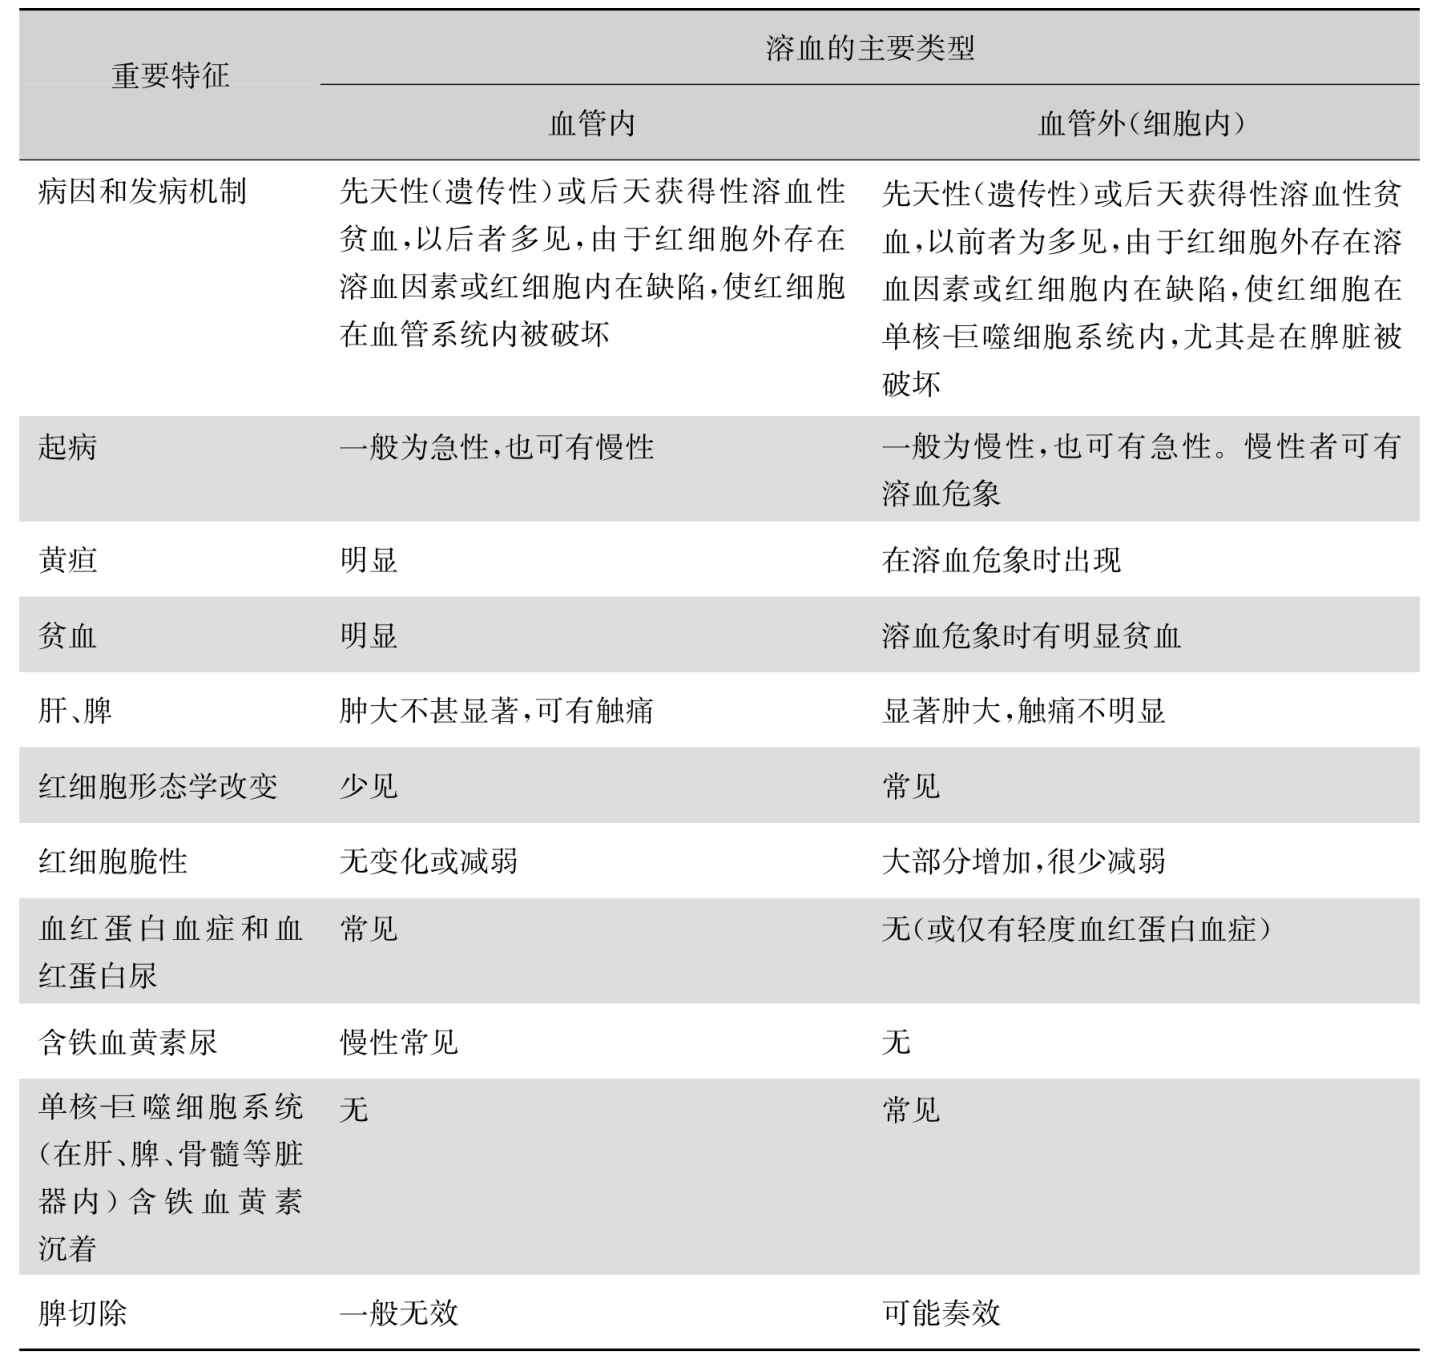
\includegraphics[width=5.95833in,height=5.66667in]{./images/Image00165.jpg}
\end{table}

\subsection{2.溶血性贫血的临床表现}

溶血性贫血按起病的急缓分为急性溶血性贫血与慢性溶血性贫血。急性溶血性贫血表现为突然发病,背痛、四肢疼痛、头痛、高热、黄疸,可有周围循环衰竭、无尿或少尿(急性肾衰竭)等。慢性溶血性贫血起病缓慢,呈慢性经过(但病程中常有病势加剧,酷似急性溶血),有轻度巩膜黄染或隐性黄疸,常伴有肝、脾大。

临床上急性溶血性贫血应与败血症区别。急性溶血性贫血,呈正色素性,中性粒细胞无中毒颗粒,骨髓以红细胞系统增生为主,血培养阴性;而败血症,贫血呈低色素性,骨髓以粒细胞系统增生为主,中性粒细胞有中毒颗粒,血培养阳性。

慢性溶血性贫血所致黄疸须与慢性黄疸型病毒性肝炎相区别。前者无肝炎接触史,消化系统症状不明显,有贫血,网织红细胞增多,肝功能检查正常,非结合胆红素升高而结合胆红素变化不大;病毒性肝炎肝功能检查异常,结合和非结合胆红素均见升高。

\subsection{3.溶血性贫血的实验室检查}

确诊溶血性贫血主要依靠实验室检查。应首先确定是否有溶血存在(表\ref{tab33-4}),然后再确定溶血的病因或类型(表\ref{tab33-5})。溶血性贫血实验室检查项目繁多,可按图\ref{fig33-1}所示,有步骤地进行检查。

\begin{table}[htbp]
\centering
\caption{溶血的实验室诊断}
\label{tab33-4}

\includegraphics[width=5.91667in,height=5.63542in]{./images/Image00166.jpg}
\end{table}

\begin{longtable}{c}
 \caption{溶血病因或类型的实验室诊断}
 \label{tab33-5}
 \endfirsthead
 \caption[]{溶血病因或类型的实验室诊断}
 \endhead
 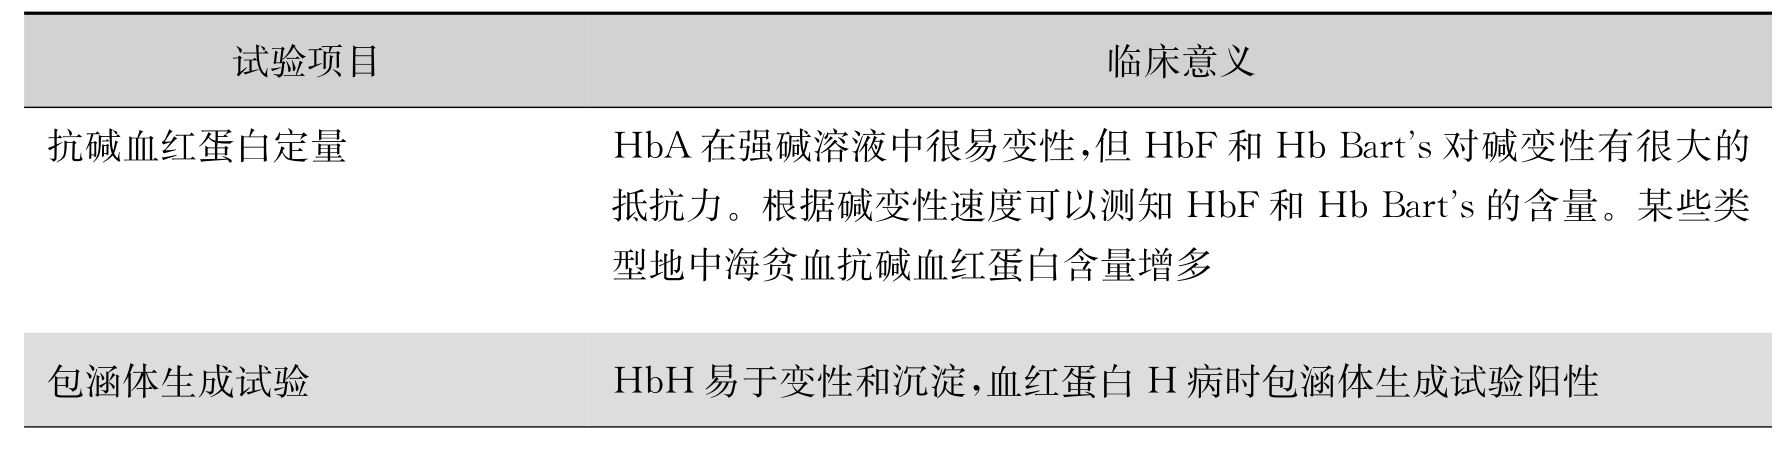
\includegraphics[width=\textwidth,height=\textheight,keepaspectratio]{./images/Image00167.jpg}\\
 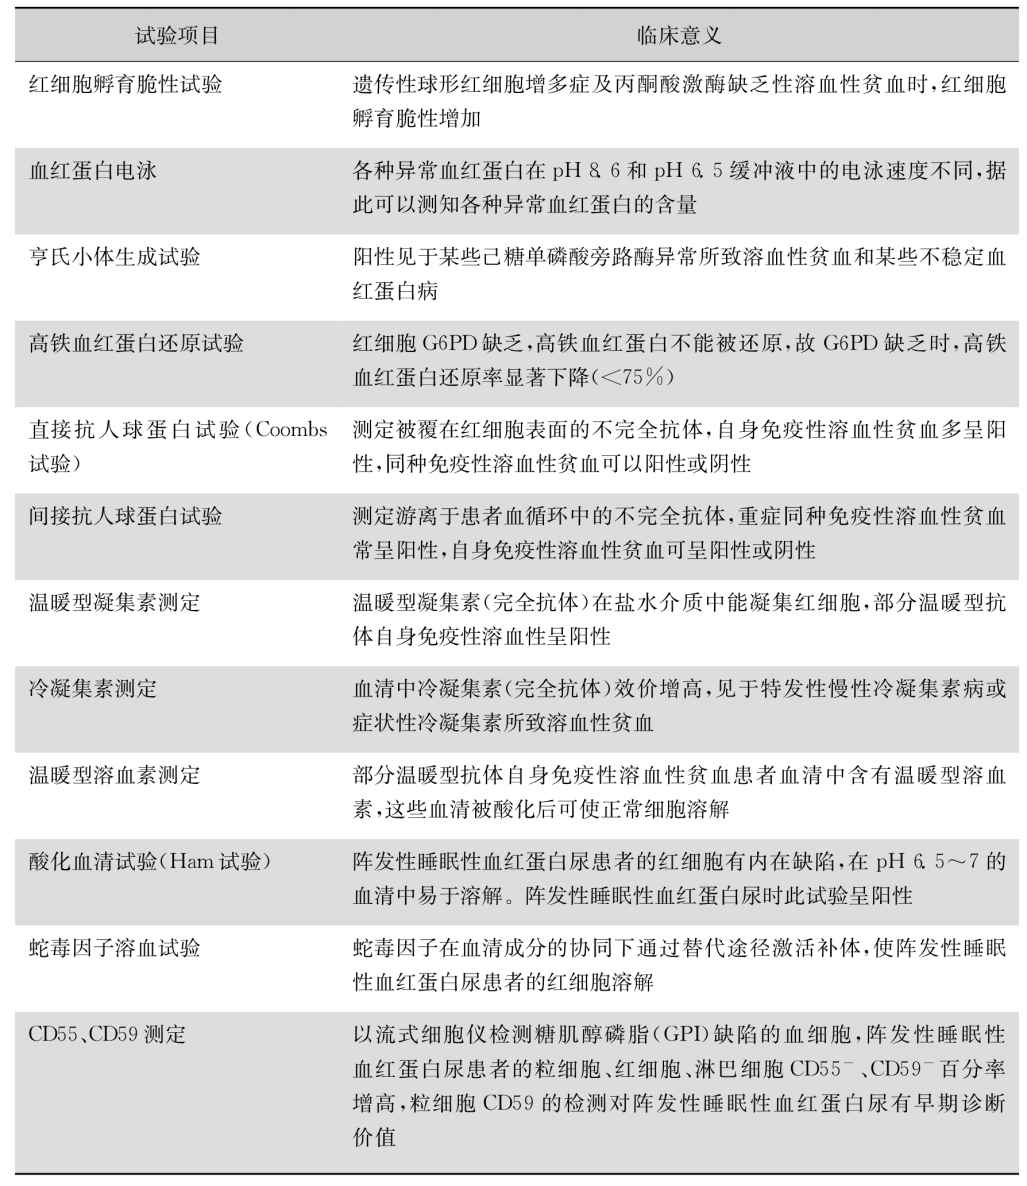
\includegraphics[width=\textwidth,height=\textheight,keepaspectratio]{./images/Image00168.jpg}
 \end{longtable}

\begin{figure}[!htbp]
 \centering
 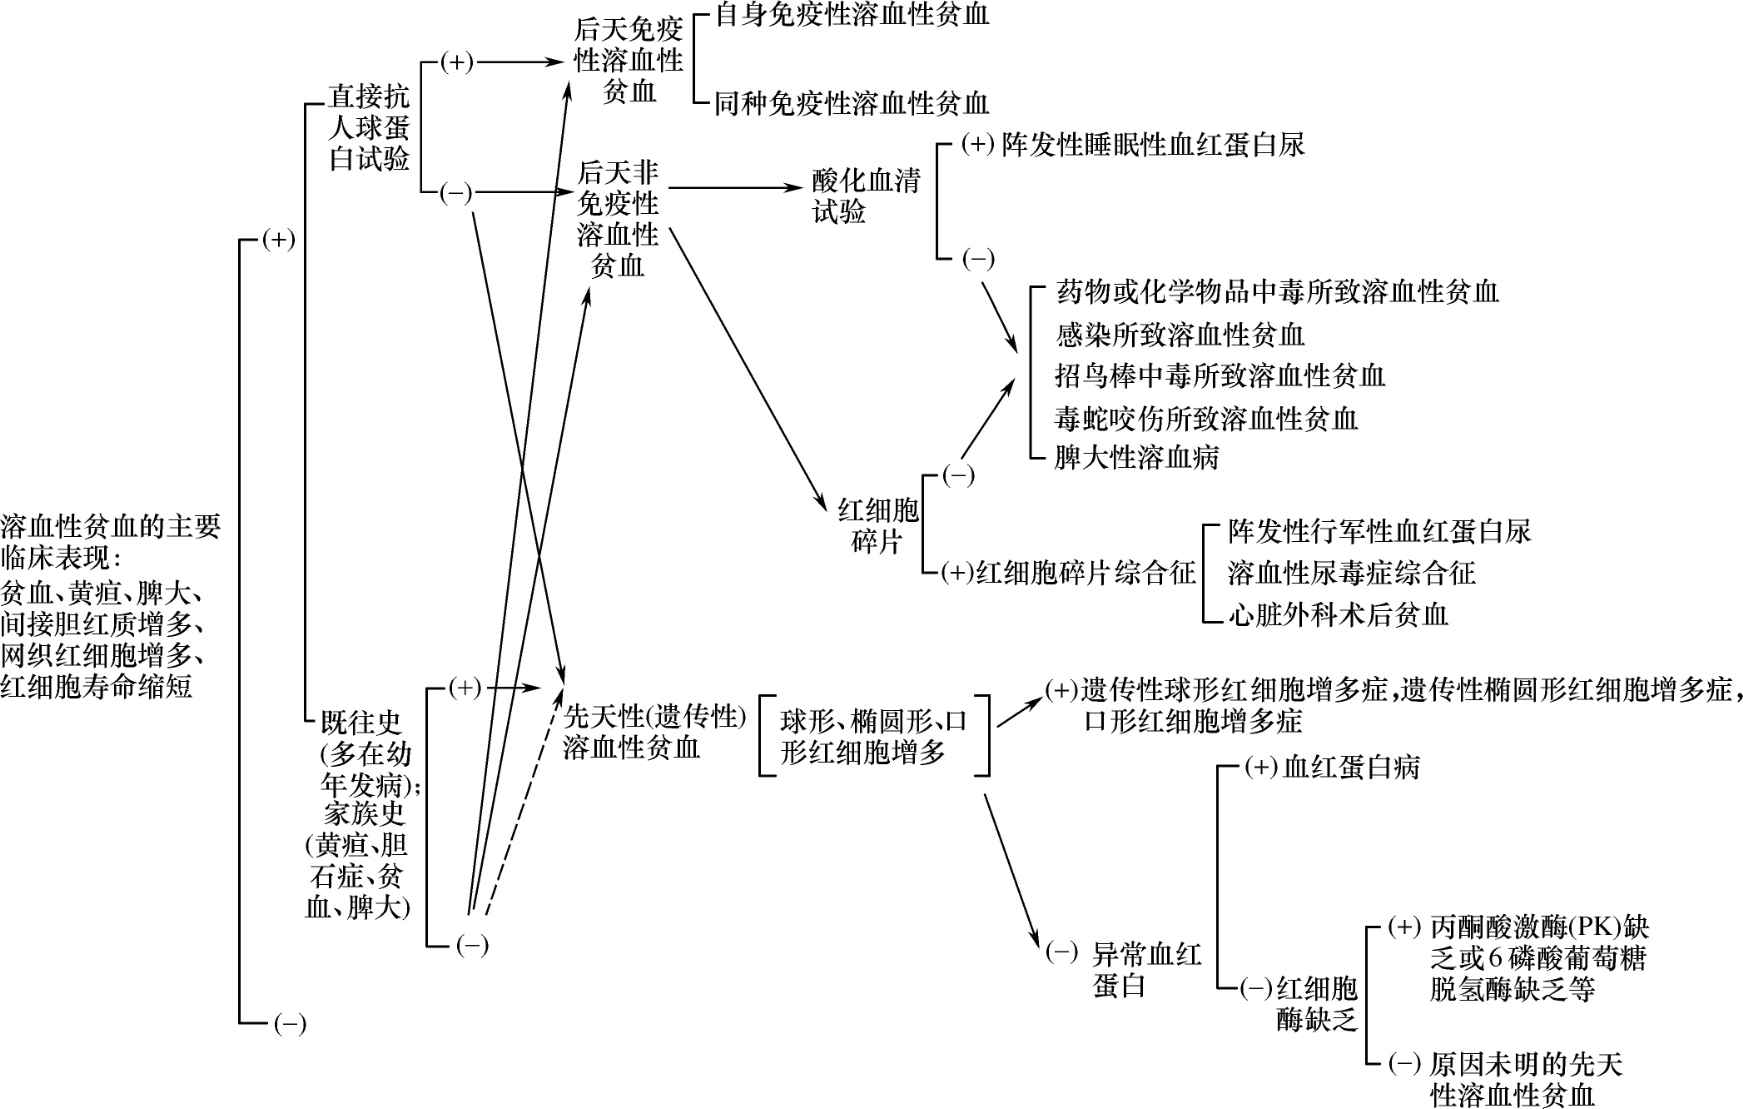
\includegraphics[width=7.25in,height=4.54167in]{./images/Image00169.jpg}
 \captionsetup{justification=centering}
 \caption{溶血性贫血病因学或类型诊断的检查步骤}
 \label{fig33-1}
  \end{figure} 

(+)表示阳性 (-)表示阴性

各类型溶血性贫血的鉴别诊断讨论如下。

\protect\hypertarget{text00259.html}{}{}

\subsection{113.1 先天性(遗传性)溶血性贫血}

临床上发现原因未明的贫血,周围血液有红细胞增生过度的表现,幼年发病而又兼有家族病史者,应考虑先天性(遗传性)溶血性贫血的可能性。此类贫血的发病原因主要是由于红细胞本身的遗传性缺陷。此类贫血的发病机制基本上可区分为三组:①血红蛋白病;②红细胞膜结构和功能异常;③红细胞酶的缺乏(图\ref{fig33-2})。

临床上发现患者自幼有难治性低色素性贫血,应考虑某些血红蛋白病的可能性。到2001年底,全世界报道的异常血红蛋白已达827种,我国进行了近100万人群的异常血红蛋白普查,已发现84种以上血红蛋白变异体,其中有35种以上为世界首次发现。β\textsuperscript{-}
地中海贫血以华南五省(广西、广东、四川、福建、贵州)最多见。

红细胞形态学的改变(球形、椭圆形及口形等),提示红细胞膜结构和功能异常所致溶血性贫血。由于对红细胞糖代谢途径的了解,已明了参与红细胞糖代谢的各种酶缺乏,可使红细胞不能维持自身的完整性而引起溶血性贫血。这类红细胞酶缺乏所致的溶血性贫血,红细胞形态正常,称为遗传性非球形红细胞性贫血。

\subsubsection{113.1.1 血红蛋白病}

血红蛋白是成熟红细胞的主要蛋白质,占细胞干重的96\%。血红蛋白由珠蛋白和血红素组成,珠蛋白由两对不同珠蛋白链构成四聚体。血红蛋白分子中的珠蛋白由两对多肽链构成。血红素由原卟啉与铁组成。正常血红蛋白是四条珠蛋白链和四个血红素分子构成的四聚体。在个体发育过程中,血红蛋白的珠蛋白链有所不同。正常成人的血红蛋白是血红蛋白A
(α2β2),占血红蛋白总量的97\%,其次是血红蛋白A2(α2δ2),占2\%~3\%,血红蛋白F(α2γ2)占1\%。

血红蛋白病包括两类疾病,一种是珠蛋白的一级氨基酸构成异常引起的异常血红蛋白病,另一种是珠蛋白合成不足所致的珠蛋白生成障碍性贫血(地中海贫血)。

异常血红蛋白病是一组遗传性珠蛋白链分子结构异常的疾病。血红蛋白的异常表现为珠蛋白链中单个氨基酸的替代(占90\%)、多个氨基酸的替代、氨基酸缺失、氨基酸插入、肽链延长及肽链融合等。目前世界上已发现并分析的异常血红蛋白达827种,我国至少发现有84种,其中35种是世界上首次发现。异常血红蛋白最初按英文字母次序命名,后发现的异常血红蛋白则以发现地的地名、民族或国名命名。虽然异常血红蛋白的种类繁多,但多数无临床症状。

镰形细胞综合征又称血红蛋白S病,其分子病理是β基因发生单一碱基突变,正常β基因第6个密码子为GAG,突变后变为GTG。临床上,镰形细胞综合征有三种表现形式:纯合子状态,即镰形细胞性贫血;杂合子状态;与其他异常血红蛋白的双杂合子状态。

不稳定血红蛋白是由于α或β珠蛋白链氨基酸组成改变致使血红蛋白分子结构不稳定,发生变性和沉淀,形成红细胞内变性珠蛋白小体(Heinz小体)。目前已发现100多种不稳定血红蛋白,80\%是β链异常。

氧亲和力增高血红蛋白是由于血红蛋白氨基酸组成的改变,使血红蛋白对氧的亲和力增高、向组织释放氧减少,导致组织缺氧、红细胞代偿性增多。

\begin{figure}[!htbp]
 \centering
 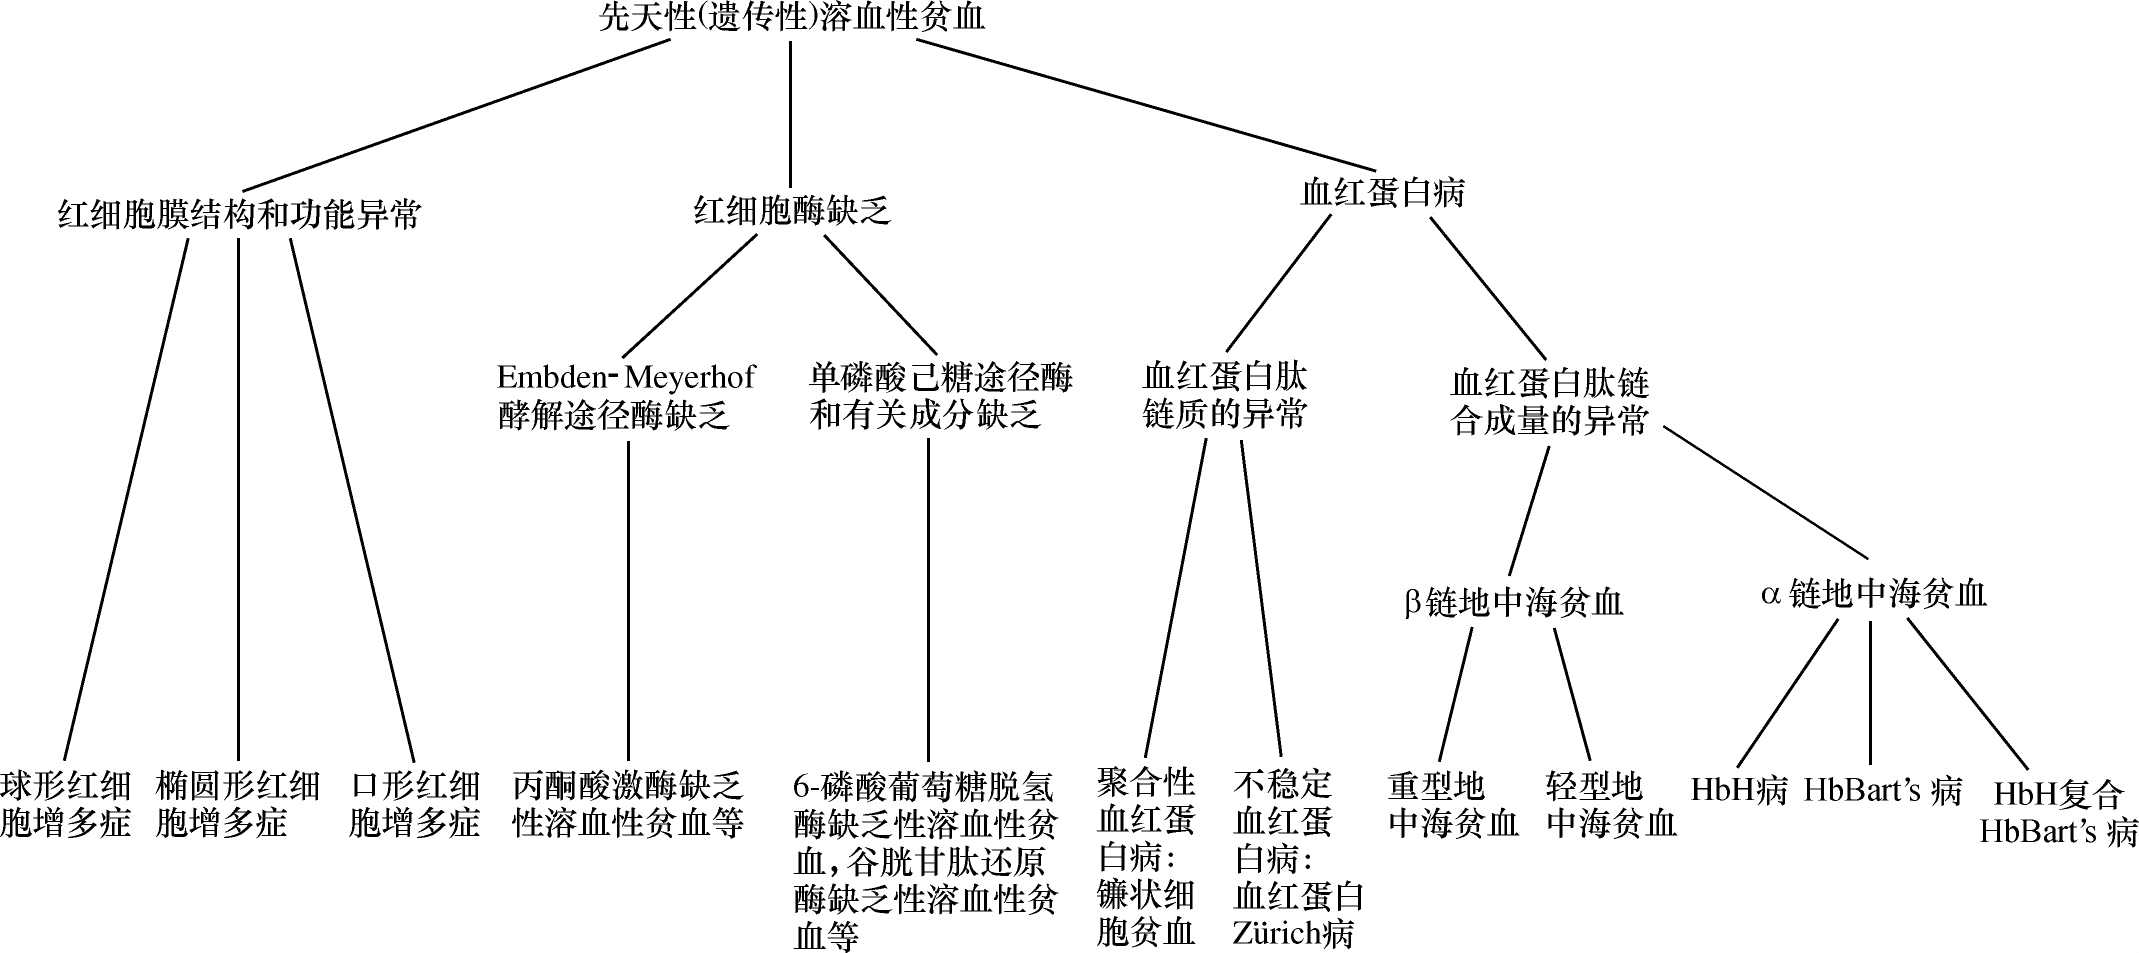
\includegraphics[width=7.3125in,height=3.29167in]{./images/Image00170.jpg}
 \captionsetup{justification=centering}
 \caption{先天性(遗传性)溶血性贫血分类}
 \label{fig33-2}
  \end{figure} 

血红蛋白M病是由于珠蛋白链氨基酸组成的改变所致的高铁血红蛋白。

珠蛋白生成障碍性贫血是指由于遗传的基因缺陷致使血红蛋白中一种或多种珠蛋白链合成缺如或不足所导致的贫血或病理状态。由于基因缺陷的复杂多样性,珠蛋白缺陷的类型、数量及临床表现不一。根据所缺乏的珠蛋白链种类及缺乏的程度进行分类,α链缺乏称为α珠蛋白生成障碍性贫血(α地中海贫血),β链缺乏称为β珠蛋白生成障碍性贫血(β地中海贫血)。

\paragraph{1.α珠蛋白生成障碍性贫血}

当α珠蛋白链合成障碍时,没有足够的α珠蛋白链与β珠蛋白链合成血红蛋白A,剩余的β链组合成血红蛋白H(β4),剩余的γ链组合成血红蛋白Bart's
(γ4)。β4亲氧力过高,不宜运输氧,且不稳定,容易发生沉淀,形成包涵体,导致溶血。γ4有极高的亲氧力,不能向组织释放足够的氧,导致胎儿缺氧死亡。根据不同的组合,α珠蛋白生成障碍性贫血分为血红蛋白H(β4)病、血红蛋白Bart's(γ4)病及血红蛋白H复合Bart's病三种类型。

\paragraph{2.β珠蛋白生成障碍性贫血}

从遗传学观点又可分为纯合子型和杂合子型。在纯合子型,β链合成没有或极少,正常血红蛋白中唯一含有β链的HbA产生受抑制,由于β链的减少,多余的α链就与γ链或δ链结合,结果血红蛋白A减少,而血红蛋白F含量明显增高,血红蛋白A2含量也增高。在杂合子型,β链合成抑制比纯合子型轻,血红蛋白A2含量增高,血红蛋白F含量轻度增高。

\paragraph{}{一、异常血红蛋白病}

\subparagraph{(一)镰状细胞综合征}

1.镰状细胞贫血%}

本病又称纯合子型镰状细胞血红蛋白病。β链第6位上的谷氨酸被缬氨酸替代后形成血红蛋白S,红细胞含有血红蛋白S,在缺氧条件下,这些血红蛋白聚合成细长的结晶,使红细胞变成镰状。镰状红细胞僵硬,变形性差,难于通过毛细血管,可引起毛细血管阻塞,导致临床上出现溶血性贫血和血栓形成。由于早年发病,患者生长和发育受影响,一般情况差,易发生感染,除有贫血、黄疸、肝脾大等症状外,常出现心肺、肾、神经系统、眼部等病变。本病在稳定时,患者尚可耐受贫血及其他症状,但当病情加重时,出现镰状细胞危象。根据临床表现的不同,可将镰状细胞危象分为五型:梗死型(疼痛型)、再生障碍型、巨幼细胞型、脾滞留型和溶血型。

本病的诊断依据:①贫血,黄疸,网织红细胞增多;②腹痛和腿痛;③脾脏于早期可肿大,但后期则不肿大(多次脾梗死形成大量瘢痕组织使脾脏缩小);④溶血危象;⑤镰变试验(sickling
test)阳性;⑥血红蛋白电泳主要成分为血红蛋白S。

感染、妊娠、外科手术可诱发溶血危象。在溶血危象并发各脏器的血栓形成(血栓性危象)时,容易造成复杂的临床病象,常可误诊为急腹症、风湿热、肺炎及骨骼系统疾病。血红蛋白电泳易作出鉴别诊断。本病尚需与其他慢性溶血性贫血相鉴别。

2.镰状细胞特性%}

镰状细胞特性又称杂合子型镰状细胞血红蛋白病。红细胞含有血红蛋白S(通常占20\%~45\%)和正常血红蛋白A,患者平时无临床症状,血象可正常,但在缺氧情况下,可有血尿、肾功能损害或肺、脾梗死的临床表现。

3.血红蛋白S-β珠蛋白生成障碍性贫血%}

血红蛋白S-β珠蛋白生成障碍性贫血又称双杂合子状态。临床表现取决于患者双杂合子的性质,若从父母一方继承了血红蛋白S基因,从另一方继承了杂合子β珠蛋白生成障碍性贫血的基因,患者尚有部分正常的β链生成,患者临床表现轻;若从父母一方继承了血红蛋白S基因,从另一方继承了纯合子β珠蛋白生成障碍性贫血的基因,患者完全没有正常的β链生成,患者临床表现与镰状细胞性贫血相似,有严重的溶血性贫血、血管梗死,常早年夭亡。

\subparagraph{(二)血红蛋白E病}

本病是一种不伴性、不完全显性遗传性疾病。血红蛋白E(HbE)是由于正常血红蛋白(HbA)的珠蛋白β链的第26个残基上,原有的谷氨酸为赖氨酸所取代而形成。血红蛋白E病纯合子型临床表现为轻度乃至中度小细胞低色素性贫血,发育正常,脾不大。血片中靶形红细胞占25\%~75\%。血红蛋白电泳检查血红蛋白E占92\%~95\%。单纯杂合子型又称血红蛋白E特征,是血红蛋白E与血红蛋白A的杂合子,患者无贫血,红细胞形态基本正常,涂片中只有少量的靶形红细胞,血红蛋白电泳检查血红蛋白E占30\%~45\%。混合杂合子型多数合并地中海贫血(血红蛋白E-地中海贫血)。血红蛋白E病在汉族、瑶族与壮族均有发现。国外以东南亚多见。国内在南方各省较多见。

\subparagraph{(三)不稳定血红蛋白病}

α珠蛋白基因或β珠蛋白基因突变导致相应的珠蛋白链氨基酸成分的改变。至今为止所发现的不稳定血红蛋白病均为杂合子,尚未见纯合子的报道。患者的异常血红蛋白分子有不稳定的理化性质,在红细胞内形成变性的珠蛋白小体,附于红细胞膜上,使膜的变形性降低,最终在脾脏中破坏。不稳定血红蛋白病有百余种,多数不稳定血红蛋白病患者,由于骨髓红系代偿性增生而不出现症状,但当发生感染或服用氧化剂类药物时,不稳定血红蛋白沉淀加剧,溶血性贫血加重。

本病特点:红细胞呈低色素性贫血,大小不均,可见多染性、嗜碱性点彩红细胞;红细胞含有变性珠蛋白小体;网织红细胞增多,与贫血不平行;高铁血红蛋白血症。不稳定血红蛋白常用的检查方法有:热变性试验、异丙醇试验、乙酰苯肼试验。异丙醇试验不仅使不稳定血红蛋白沉淀,也可使血红蛋白F沉淀,应注意鉴别。血红蛋白电泳在鉴别不稳定血红蛋白上作用有限。

不稳定血红蛋白病的红细胞,多含有变性珠蛋白小体。变性珠蛋白小体并非本病所特有,在6-磷酸葡萄糖脱氢酶(G6PD)缺乏所致药物性溶血性贫血及血红蛋白H病中,其红细胞内也有变性珠蛋白小体形成,须与本病区别。6-磷酸葡萄糖脱氢酶缺乏时,血红蛋白并不具有热不稳定性,6-磷酸葡萄糖脱氢酶活性减低,可与不稳定血红蛋白病相区别。血红蛋白热不稳定性测定方法(热变性试验):将溶血产物加温至50℃,可见不稳定血红蛋白的沉淀物。血红蛋白H的分子虽有不稳定的理化性质,但其肽链结构并无异常,根据血红蛋白电泳法可与本病区别。

\subsubsection{二、珠蛋白生成障碍性贫血}

\subparagraph{(一)β珠蛋白生成障碍性贫血}

β珠蛋白生成障碍性贫血原名地中海贫血,本病广泛分布于世界各地,东南亚是高发地区之一,我国广东、广西、四川较多见,长江以南各省、市有散发病例。

本病是显性(或隐性)基因遗传性疾病。从遗传学观点可分为两型:

1.纯合子型%}

自父母双方各继承了一个异常β基因,没有或极少β链合成,病情较重。

2.杂合子型%}

自父母一方继承了一个异常β基因,从另一方继承了一个正常β基因,有半量β链合成,病情较轻。

纯合子型病例的临床特点:①有家族病史或地域史,幼年发病;②严重溶血性贫血,发育不良,呈呆滞面容;③肝轻度或中度大,脾明显大;④血液学改变表现为小细胞低色素性贫血,外周血出现大量靶形红细胞,并有或多或少的有核红细胞,网织红细胞增多,红细胞脆性降低,血清非结合胆红素升高,骨髓象呈增生活跃,红系显著增多,铁染色显示含铁血黄素颗粒和铁粒幼细胞增多;⑤X线颅骨及长短骨照片检查可见颅骨及长短骨髓腔增宽,骨质疏松,骨皮质变薄,颅骨骨小梁条纹清晰呈辐射状或直毛发样排列。

杂合子型病例大多无明显临床症状,通常无贫血,一般在普查或合并有其他疾病进行检查时发现,检查可见或有轻度小细胞性低色素性贫血,靶形红细胞增多,红细胞脆性降低。

血红蛋白电泳或碱变性试验见血红蛋白F显著增高,对诊断纯合子型β珠蛋白生成障碍性贫血有重要意义。血红蛋白电泳示血红蛋白A2含量增高(3\%~8\%),血红蛋白F正常或轻度增高(<5\%),对诊断杂合子型β珠蛋白生成障碍性贫血病例有重要意义。

虽然血红蛋白F(胎儿血红蛋白)增多对诊断重型β珠蛋白生成障碍性贫血有重要意义,但仍需结合临床及其他化验检查,进行全面分析,才能确诊。因在某些恶性肿瘤、再生障碍性贫血和白血病等,其胎儿血红蛋白含量也可升高,甚至可达35\%,但血红蛋白A2多下降,可作为鉴别诊断。重型β珠蛋白生成障碍性贫血尚需与高血红蛋白F综合征相鉴别。后者除血红蛋白F含量明显增高外(常在30\%以上),无任何临床症状,血象也基本正常,这些特点显然与重型β珠蛋白生成障碍性贫血不同,两者的鉴别不难。

本病因属小细胞性低色素性贫血,还应与缺铁性贫血相鉴别。在缺铁性贫血,多有引起缺铁的原因或病史,红细胞的异常增生现象较轻,靶形红细胞增多不显著,红细胞脆性减低不明显,血清铁、铁蛋白低,铁粒幼细胞减少,无家族病史及其他溶血征象,用铁剂治疗有效,据此可与地中海贫血相鉴别。

\subparagraph{(二)α珠蛋白生成障碍性贫血}

1.胎儿水肿综合征%}

胎儿父母均为α珠蛋白生成障碍性贫血的杂合子,胎儿继承了父母双方有缺陷的α基因,即4个α基因均缺失,正常胎儿血红蛋白(血红蛋白F)缺如,红细胞内含有多量血红蛋白Barts(γ4),这种异常的血红蛋白与氧结合很紧密,向组织释放氧很少,导致胎儿窒息死亡。本病胎儿大多在妊娠30~40周时成为死胎或早产后数小时死亡。

2.血红蛋白H病%}

患者自父母双方继承了不同的异常α基因,有3个α基因异常,仅能生成少量的α珠蛋白链,无足够α链配对的β链自行聚合成β4四聚体(血红蛋白H)。患者出生时可有轻度贫血,临床表现似轻型β链地中海贫血。由于血红蛋白H(β4)的分子具有不稳定性质,患者接触某些化学物品或药物,可加重溶血。

3.α珠蛋白生成障碍性贫血性状%}

患者是正常α基因与异常α基因的杂合子,分为静止型和标准型。由于仅有轻度的α珠蛋白链缺失,患者可无贫血或其他症状,没有或仅有轻度的红细胞形态改变,偶见血红蛋白H,测定α/β链合成比率可以明确诊断。

含有血红蛋白H的红细胞,在活体染色条件下,可见红细胞包涵体;用含有氧化作用的染色剂孵育,可见变性珠蛋白小体形成。血红蛋白Bart's则可用血红蛋白抗碱试验检出。上述三项检验如为阳性,则强烈提示本病的可能性。血红蛋白电泳发现血红蛋白H和血红蛋白Bart's则可确诊。

\subsubsection{113.1.2 先天性(遗传性)红细胞膜结构和功能异常}

\paragraph{一、遗传性球形红细胞增多症}

本病又名先天性(或家族性)溶血性黄疸,是一种红细胞膜蛋白基因异常的常染色体显性遗传性疾病,少数为非显性或隐性遗传。常有明显的家族病史。遗传性球形红细胞增多症见于世界各地,北欧及美国发病率较高,本病是我国最多见的遗传性膜缺陷病。患者的红细胞膜有先天性异常,表现为红细胞膜的脆性增加而易在脾内滞留遭受破坏;另一方面的缺陷表现为红细胞膜对钠盐进入细胞的通透性增加,导致ATP的损耗,这也可能为溶血原因之一。

贫血、黄疸、脾大是遗传性球形红细胞增多症最常见的临床表现,三者可同时存在或先后出现。感染、持久的体力劳动会增加脾的血流量,可加重溶血。根据不同的临床表现,遗传性球形红细胞增多症分典型遗传性球形红细胞增多症、轻型遗传性球形红细胞增多症、无症状携带者和重型遗传性球形红细胞增多症。

本病确诊除结合病史、临床表现外,尚需依靠以下血液学检查:①外周血片小球形红细胞增多,占10\%以上;②红细胞渗透脆性实验:开始溶血或(和)完全溶血的盐水浓度超过正常对照的0.08\%以上;③48小时自身溶血试验:溶血超过5\%,葡萄糖或ATP能明显减少溶血;④酸化甘油溶血试验阳性。

虽然外周血出现小球形红细胞增多和红细胞渗透脆性增高是遗传性球形红细胞增多症的两大特征,但也可见于温抗体型自身免疫性溶血性贫血、新生儿ABO血型不相容性贫血、G6PD缺乏症、不稳定血红蛋白病等,脾切除可使遗传性球形红细胞增多症贫血减轻,但温抗体型自身免疫性溶血性贫血也有效,需进行鉴别。

溶血危象的发作常表现为畏寒、发热、黄疸、脾大与腹痛,红细胞数迅速下降,常因感染而诱发,易被误诊为胆道感染。如患者在腹痛同时,还有贫血、小腿溃疡、家族病史,则强烈支持本病而不支持胆道感染。本病可同时合并胆石症,因此,如患者有胆绞痛史,作切脾手术治疗时,应同时探查胆囊,以排除并存胆石症的可能性。

由于本病以黄疸为常见症状,故易误诊为Gilbert综合征或先天性遗传性非球形红细胞贫血,鉴别诊断参考表\ref{tab33-6}。

\begin{table}[htbp]
\centering
\caption{先天性(遗传性)非球形红细胞贫血、遗传性球形红细胞增多症、免疫性溶血性贫血、Gilbert综合征的鉴别诊断}
\label{tab33-6}
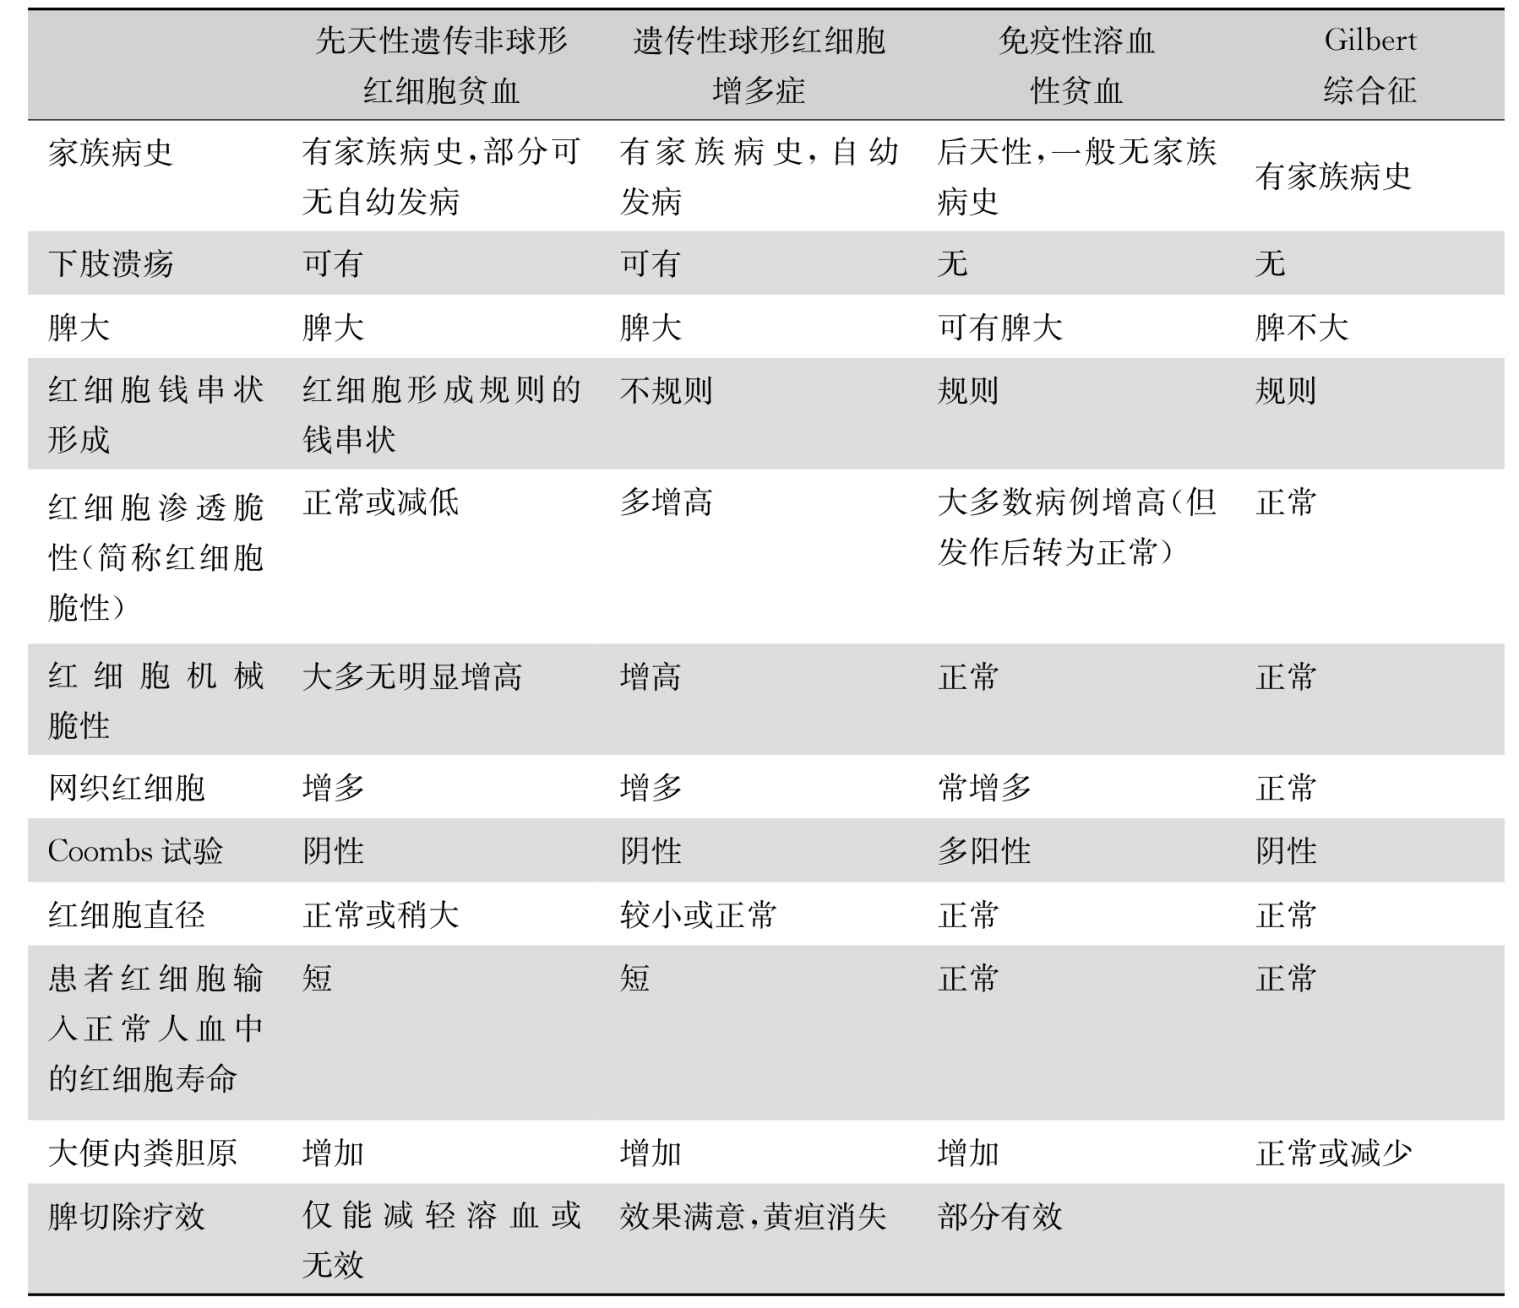
\includegraphics[width=5.98958in,height=5.15625in]{./images/Image00171.jpg}
\end{table}

\paragraph{二、遗传性椭圆形红细胞增多症}

遗传性椭圆形红细胞增多症是一组异质性家族性常染色体显性遗传性疾病,特点是外周血中有大量的椭圆形成熟红细胞。目前认为,本病是一组由于红细胞膜蛋白异常引起的遗传性溶血病,临床上分为四种类型:普通型遗传性椭圆形红细胞增多症、遗传性热变性异形红细胞增多症、球形细胞性遗传性椭圆形红细胞增多症、口形细胞性遗传性椭圆形红细胞增多症。

遗传性椭圆形红细胞增多症患者临床表现可轻重不等,有的除红细胞形态异常外,没有临床异常表现,仅10\%~15\%可有显著溶血的表现,少数病例可因感染而诱发溶血危象。偶见慢性小腿溃疡形成。少数症状明显的病例,可有脾大。

根据临床表现、红细胞形态和家族调查,大多数患者可明确诊断。椭圆形红细胞在正常人很少超过15\%,本病时可达60\%~90\%。一般认为>25\%时有诊断意义,如无家族史,外周血椭圆形红细胞>50\%时有诊断意义。另外,椭圆形红细胞也可见于其他血液系统性疾病,如缺铁性贫血、骨髓纤维化、骨髓病性贫血、骨髓增生异常综合征、巨幼细胞性贫血、珠蛋白生成障碍性贫血和丙酮酸激酶缺乏症等,上述疾病除有椭圆形红细胞外,常有其他特殊的异形细胞和临床征象可资鉴别。

\paragraph{三、口形红细胞增多症}

本病属常染色体显性遗传性溶血病。主要病变是细胞内钠含量显著增高,大量钠内流导致细胞水肿、肿胀,体积增大,ATP利用增加,葡萄糖消耗增加,乳酸堆积。血液学特点是:红细胞内有一条像鱼嘴样的中心苍白区(超过5\%),而在血片上则呈碗形。临床上可有中、重度溶血性贫血,外周血口形红细胞达10\%~30\%,红细胞渗透脆性增加,脾切除无效。

\subsubsection{113.1.3 先天性(遗传性)红细胞酶缺乏}

先天性(遗传性)红细胞酶缺乏又称红细胞酶病,是指参与红细胞代谢的酶由于基因缺陷,导致活性改变而发生溶血的一组疾病。近年来由于对红细胞糖代谢途径的进一步了解,因而陆续发现多种红细胞酶缺乏所致的溶血性贫血。目前已知19种因酶缺陷、1种因酶活性增高引起的溶血,这些酶分布于红细胞无氧糖酵解途径、红细胞磷酸戊糖旁路、谷胱甘肽代谢和红细胞核苷酸代谢。这类贫血主要分为两大类:①无氧酵解途径的酶缺乏;②己糖磷酸旁路途径酶和有关成分的缺乏(见图\ref{fig33-3})。这两类溶血性贫血患者的红细胞不呈球形,且脆性正常,故其中某些种类的贫血又称先天性(遗传性)非球形红细胞贫血。

成熟红细胞的糖代谢:成熟红细胞不含糖原,必须经常摄取葡萄糖,以保证一定的能量代谢,有效维持其正常生理功能。葡萄糖自血浆进入红细胞后,主要通过两种途径进行代谢:无氧酵解途径(EMP)及己糖磷酸旁路途径(HMP)。无氧酵解途径起主要供能作用:每分子葡萄糖经过酵解途径,能产生两个三磷酸腺苷(ATP)。ATP是“钠-钾泵”的重要能源,对维持红细胞的完整性有很重要的作用。当这一途径中某种酶缺乏时(丙酮酸激酶、己糖激酶缺乏),糖代谢发生障碍,导致ATP生成不足,从而无法维持红细胞膜上钠、钙泵的运转,破坏了红细胞内的离子平衡和红细胞膜的柔韧性,细胞形态发生改变,导致红细胞溶解。另一途径己糖磷酸旁路途径则是需氧途径,红细胞内约5\%~10\%的葡萄糖进入该通路。与无氧糖酵解途径不同,磷酸己糖通路不产生任何高能磷酸键,此通路的功能在于还原NAPD\textsuperscript{+}
为还原型辅酶Ⅱ(NAPDH),后者是谷胱甘肽还原酶(GR)及高铁血红蛋白还原酶反应所必需。通过此反应,氧化型谷胱甘肽(GSSH)还原为还原型谷胱甘肽(GSH),变性血红蛋白和高铁血红蛋白还原为氧合血红蛋白,以抵抗H\textsubscript{2}
O\textsubscript{2}
和游离基团(红细胞自然产生或与药物接触后产生)的氧化作用,维持红细胞的完整性。当NADPH和GSH不足时,红细胞膜的稳定性即遭到破坏。综上所述,任何引起ATP或NADPH生成障碍的红细胞酶缺乏或缺陷,均可影响红细胞的正常代谢和功能,导致红细胞酶病。

\begin{figure}[!htbp]
 \centering
 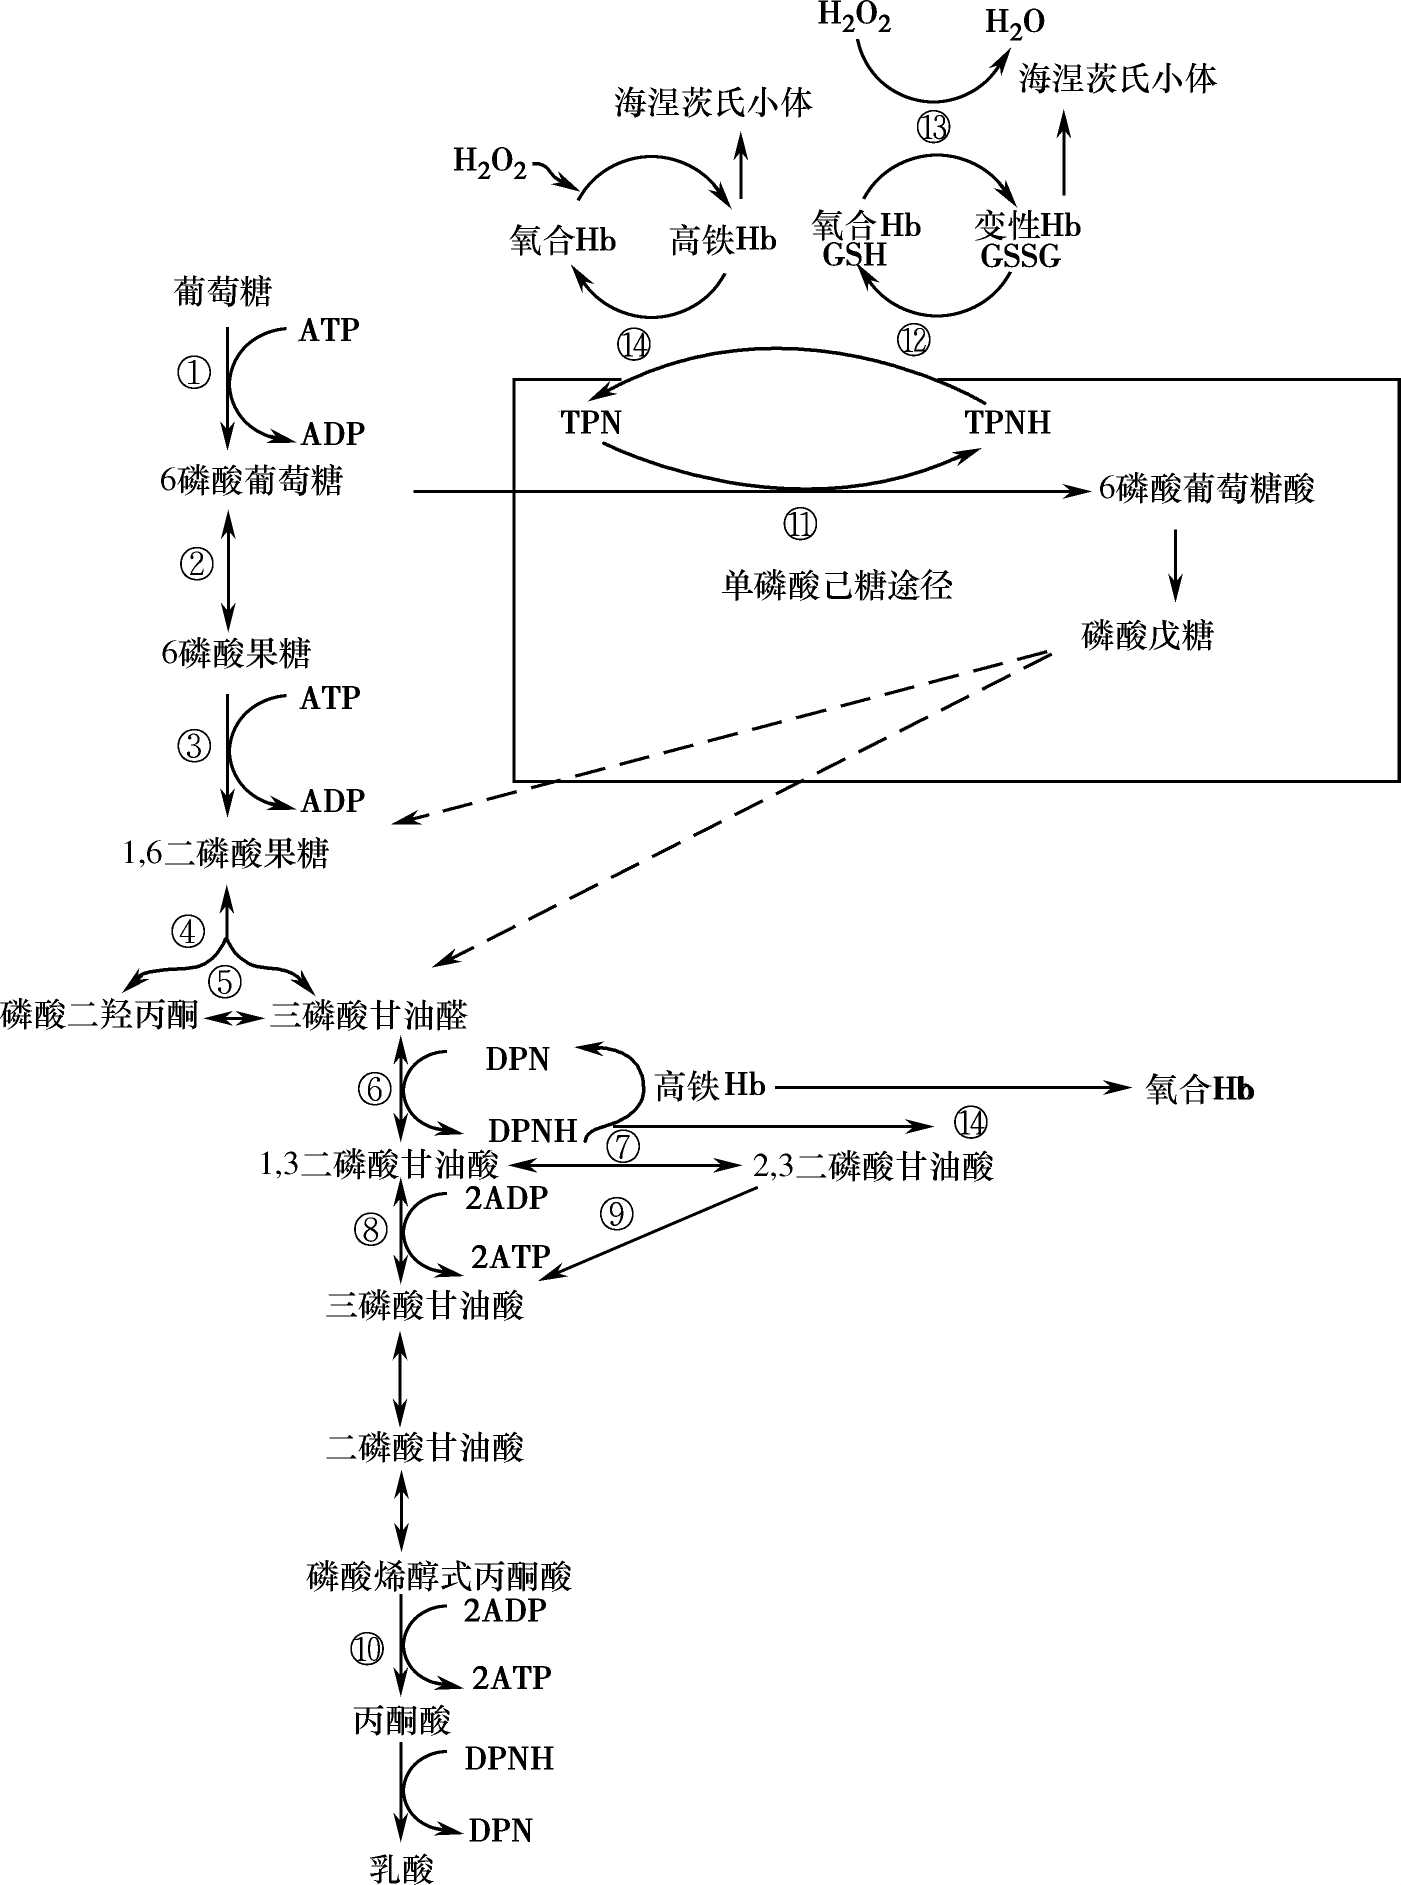
\includegraphics[width=5.01042in,height=6.38542in]{./images/Image00172.jpg}
 \captionsetup{justification=centering}
 \caption{成熟红细胞糖代谢途径及其酶缺乏图解}
 \label{fig33-3}
  \end{figure} 

圆圈内数字代表酶缺乏种类及其作用部位:①己糖激酶;②葡萄糖磷酸异构酶;③磷酸果糖激酶;④磷酸果糖醛缩酶;⑤丙糖磷酸异构酸;⑥磷酸甘油醛脱氢酶;⑦二磷酸甘油变位酶;⑧磷酸甘油激酶;⑨2,3二磷酸甘油磷酸酶;⑩丙酮酸激酶(PK)\textcircled{11}
6磷酸葡萄糖脱氢酶(G6PD)\textcircled{11}
谷胱甘肽还原酶 ;\textcircled{13}
谷胱甘肽过氧化物酶 \textcircled{14}
高铁血红蛋白还原酶。ATP三磷酸腺苷;ADP二磷酸腺苷;DPN二磷酸吡啶核苷;DPNH还原型二磷酸吡啶核苷;TPN三磷酸吡啶核苷;TPNH还原型三磷酸吡啶核苷;GSH还原型谷胱甘肽;GSSG氧化型谷胱甘肽;E-M(Embden-Meyerhof)。虚线示某些步骤被省略

\paragraph{一、参与无氧糖酵解途径的酶缺乏}

\subparagraph{(一)丙酮酸激酶缺乏症}

本病又名先天性(遗传性)非球形红细胞性贫血(Ⅱ型),是红细胞无氧糖酵解通路中最常见的红细胞酶病,属常染色体隐性遗传。纯合子和双重杂合子表现为溶血性贫血,单纯杂合子可没有临床表现。患者的红细胞缺乏丙酮酸激酶(PK),这是参与催化酵解途径的一种重要激酶。在葡萄糖无氧酵解的过程中,该酶催化磷酸烯醇式丙酮酸(PEP)转变为丙酮酸,同时ADP转变为ATP。PK缺乏时红细胞内ATP生成不足,导致红细胞膜的离子通透性增加,K\textsuperscript{+}
大量外流,使红细胞内渗透压降低,细胞内水丧失,细胞体积变小,因而出现各种皱缩红细胞。这些皱缩红细胞相互之间黏度增加,难于通过脾窦而被破坏,从而导致溶血。患者多有家族病史,多于新生儿或婴儿期发病。脾大及血涂片发现皱缩红细胞,提示本病的可能性。

本病的临床特点:①本病虽属遗传性,但可无家族病史;②主要表现为慢性溶血性贫血(贫血、黄疸和脾大),严重者可在婴儿早期出现中度以上的贫血和黄疸,需多次输血才能存活。但也有患者贫血表现很轻微,一直到青少年或成人才出现;③外周血涂片可见皱缩红细胞和有核红细胞;④红细胞脆性正常;⑤自身溶血试验多阳性,经48小时的盐水温育可见明显的溶血增加,加入葡萄糖不能纠正;⑥红细胞不含异常血红蛋白;⑦红细胞丙酮酸激酶缺乏,这是确诊该病的主要实验室依据;⑧脾切除术治疗可改善病情,使血红蛋白增加10~20g/L,减少输血次数,但不能治愈本病。诊断主要根据病史和实验室检查,如果患者有溶血的证据,有PK活性缺乏,即可诊断本病。

本病与遗传性球形红细胞增多症有时鉴别不易,其主要鉴别点为前者溶血程度常较重,红细胞脆性正常,自身溶血试验溶血不被葡萄糖纠正,而遗传性球形红细胞增多症的溶血则明显地被葡萄糖所纠正。有条件时作酶活性测定,对两者的鉴别诊断有决定性意义。本病与先天性(遗传性)G6PD缺乏性溶血性贫血、遗传性球形红细胞增多症的实验室鉴别诊断参考表\ref{tab33-7}。

\begin{table}[htbp]
\centering
\caption{先天性非球形红细胞性贫血与遗传性球形红细胞增多症的实验室鉴别诊断}
\label{tab33-7}
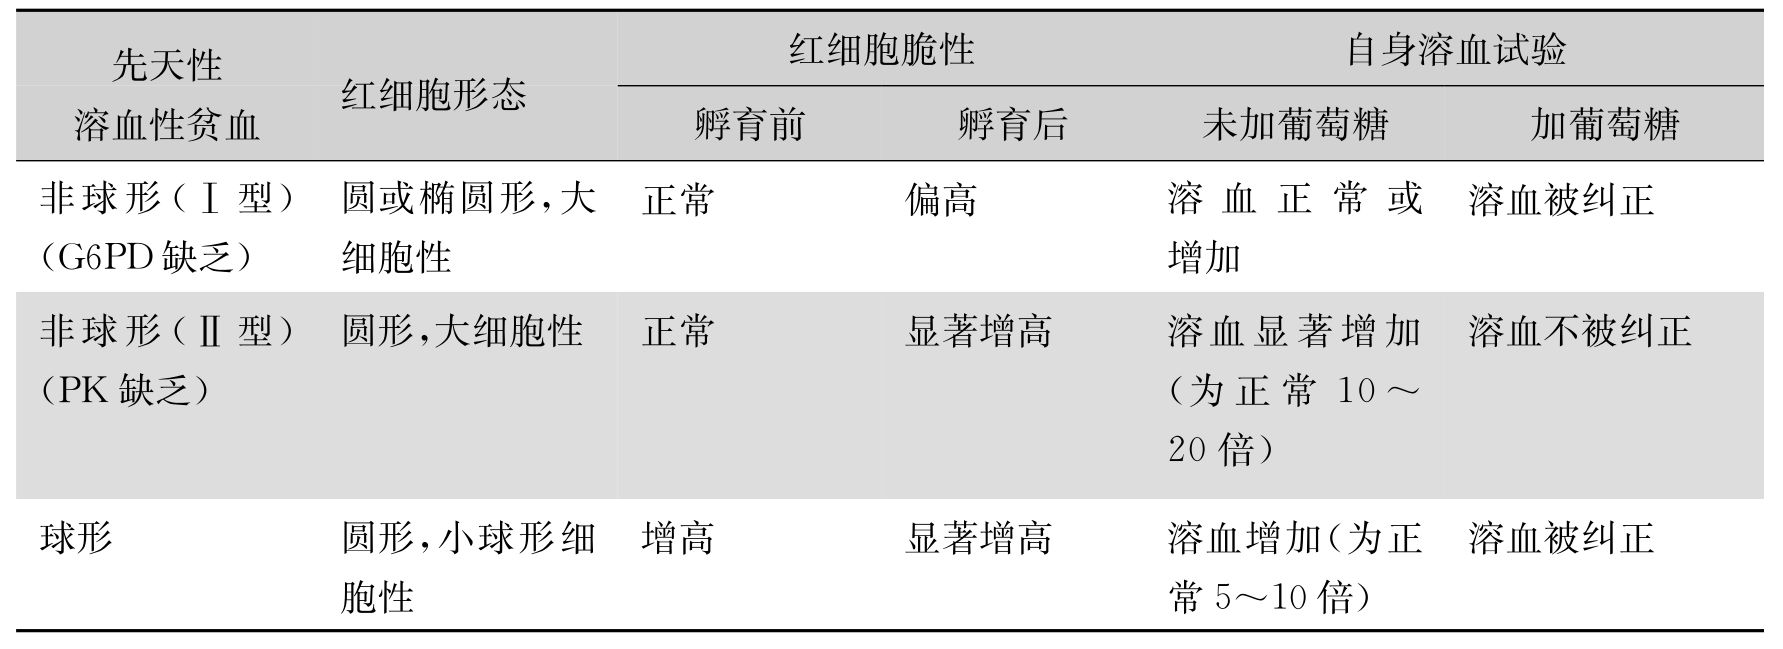
\includegraphics[width=5.9375in,height=2.15625in]{./images/Image00177.jpg}
\end{table}

\subparagraph{(二)其他酵解酶缺乏所致的先天性(遗传性)溶血性贫血}

其他酵解酶(glycolytic
enzymer)包括己糖激酶(hexokinase),葡萄糖磷酸异构酶(glucosephosphate
isomerase),丙糖磷酸异构酶(triosephosphate
isomerase),磷酸果糖激酶(phosphofructokinase),二磷酸甘油变位酶(diphosphoglycerate
mutase),磷酸甘油激酶(phosphoglycerate
kinase),磷酸果糖醛缩酶(phosphofructoaldolase)。三磷酸甘油醛脱氢酶(glyceraldehyde-3-phosphate
dehydrogenase)及2,3-二磷酸甘油磷酸酶(2,3-diphosphoglycerate
phosphatase)等也参与糖酵解途径。这些酶缺乏引起的溶血性贫血国外已有报告。这些溶血性贫血的临床表现类似先天性(遗传性)丙酮酸激酶缺乏性溶血性贫血。作有关酶的活性测定,有助于这些溶血性贫血类型的鉴别诊断。

\paragraph{二、参与己糖磷酸途径和谷胱甘肽代谢的酶缺乏}

\subparagraph{(一)葡萄糖-6-磷酸脱氢酶(G6PD)缺乏症}

是指红细胞G6PD活性降低和(或)酶性质改变导致以溶血为主要表现的疾病。其导致溶血的机制主要为,在G6PD缺乏时,由于NADPH生成不足,GSSG还原为GSH速率减慢,红细胞内GSH下降,细胞内过氧化氢酶(Cat)的抗氧化活性亦降低,因而在摄入氧化药物或感染等氧化损伤加重的情况下,血红蛋白和红细胞膜均易于发生损伤。血红蛋白氧化损伤的结果,导致Heinz小体及高氧血红素生成;红细胞膜的过氧化损伤可表现为膜脂质和膜蛋白巯基的氧化。上述改变导致红细胞膜通透性增加、红细胞变形能力降低,从而引起溶血的发生。大多数红细胞G6PD缺乏者无临床表现,有溶血的患者与一般溶血性疾病的临床表现大致相同。G6PD缺乏所致溶血性贫血有以下5种临床类型。

1.先天性非球形红细胞性溶血性贫血(CNSHA)%}

是一组红细胞酶缺陷所致的慢性溶血性贫血,其中约1/3病例由G6PD缺乏所致。主要表现为不同程度的慢性自发性血管外溶血,在感染或药物存在时溶血加重,引起溶血危象或再障危象。重型患者新生儿期发病,呈持续性溶血性黄疸一至数月,幼儿期呈中至重度贫血,多数肝脾大明显。轻型青年期发病,平时无明显贫血症状,感染、药物可诱发轻度溶血性黄疸及贫血。中间型介于两者之间,儿童或青少年期发病,每于感染诱发急性溶血性黄疸后呈慢性轻至中度溶血性贫血,无明显肝脾大。本病临床表现与PK缺乏性溶血性贫血相似,但有以下特点,可与PK缺乏性溶血性贫血相区别:①血涂片无皱缩红细胞出现;②慢性溶血性贫血,药物、感染与糖尿病酮血症可使溶血加重;③自身溶血试验溶血正常或增加,能被葡萄糖或ATP所纠正;④高铁血红蛋白还原试验还原速度减慢;⑤红细胞G6PD活性减低。

高铁血红蛋白还原试验证明红细胞G6PD缺乏,对本病诊断有一定意义。G6PD缺乏时,NADPH生成不足,高铁血红蛋白在NADPH不足的条件下还原受障碍。故G6PD缺乏时,高铁血红蛋白还原速度显著减慢(图\ref{fig33-3})。但须注意的是,如患者处于康复期,新生红细胞(网织红细胞)增多,酶不表现缺乏,此试验结果可呈假阴性。此试验也可能反映高铁血红蛋白还原酶缺乏,故只能作为一种筛选试验。

2.蚕豆病%}

是指G6PD缺乏患者食用蚕豆、蚕豆制品或接触蚕豆花粉后所发生的急性溶血性贫血。蚕豆导致溶血是由于蚕豆中含有的某些物质及其衍生物如蚕豆嘧啶和异脲脒具有氧化剂性质(在体内能产生较多的活性氧),其作用于G6PD缺乏的红细胞,造成红细胞膜的脂质过氧化损伤而致溶血。本病有明确的食蚕豆诱发溶血史。吃蚕豆后1~2天,出现精神不振、黄疸及酱油色样尿,提示本病的诊断。

蚕豆病是我国农村中比较常见的溶血性贫血。据目前所知,在国内分布颇广,广东、四川、湖南、广西、云南、贵州、福建、浙江、江苏、江西、安徽等省(自治区)均有发现,尤以广东为多见。往往发生于蚕豆扬花与收获的季节,华南地区为三月下旬至四月上旬。各年龄均可罹病,但2/3病例为9周岁以下的小儿。此酶的缺乏是按照伴性遗传规律传给后代,故男性发病显著高于女性,其比率约7∶1。

本病的临床特点是:①约1/3患者有同样的既往病史,可多次反复发病。②有家族病史的病例多达40\%。③前驱症状有发热、全身不适、头晕、乏力,消化系统症状如食欲不振、恶心、呕吐等,持续1~2天;继而发生急性溶血性贫血,出现急剧面色苍黄、黄疸、酱油样小便。④部分病例可有肝、脾大。⑤严重者嗜睡,甚至昏迷,发生失水和酸中毒。⑥实验室检查显示红细胞数与血红蛋白量下降,白细胞数增多及中性粒细胞核左移,网织红细胞增多,红细胞内可出现Heinz小体。

本病的诊断根据是:①患者有食蚕豆史、溶血性黄疸的家族病史及既往史;②呈急性血管内溶血经过;③高铁血红蛋白还原试验还原速度减慢;④红细胞G6PD活性减低。

3.葡萄糖-6-磷酸脱氢酶(G6PD)缺乏所致的药物性溶血性贫血%}

本病发生于红细胞缺乏G6PD的基础上,患者有明确的服用氧化性药物史。目前已明确的可引起G6PD缺乏者溶血的药物,有抗疟药(伯氨喹、扑疟喹啉)、磺胺类(磺胺甲唑、磺胺吡啶、对氨苯磺酰胺)、解热镇痛药(乙酰苯胺类)等,这些药物在G6PD缺乏的患者,应禁忌使用。其他还有些药物如氯喹、奎宁、磺胺甲嘧啶、阿司匹林、非那西丁等,目前认为在非CNSHA患者,在常规治疗剂量下不引起溶血,只有在超过治疗用量或患者合并有感染或同时使用其他氧化性药物时方引起溶血。这些药物引起溶血的机制为在体内代谢所产生的中间产物有氧化剂的作用,从而使患者还原能力已有缺陷的红细胞发生氧化性损伤。

临床表现视药物剂量和机体状态的不同而有差异。溶血一般在服药后48~96小时出现。溶血有自限性,约在7~10天后消退,可能与富含G6PD的新生红细胞与网织红细胞代偿性出现于周围血有关。在发病初期,常出现贫血、黄疸和血红蛋白尿。实验室检查高铁血红蛋白还原速率减慢,红细胞Heinz小体生成试验阳性,谷胱甘肽含量下降,G6PD活性下降。除药物剂量可影响溶血程度以外,糖尿病酸中毒、低血糖状态、病毒或细菌感染也可使溶血加剧。有人认为感染时,由于吞噬性白细胞产生过氧化物而激发溶血。

药物性溶血性贫血的诊断除病史外,主要依靠实验室检查。实验室诊断方法有:①G6PD活性测定;②谷胱甘肽稳定试验;③红细胞Heinz小体计数;④亮甲酚蓝染料还原试验;⑤高铁血红蛋白还原试验。其中以G6PD活性测定最为可靠。

4.G6PD缺乏所致新生儿高胆红素血症%}

是新生儿(特别是男婴)核黄疸最常见原因之一。G6PD缺乏的新生儿和正常的新生儿在出生时,血清胆红素浓度无显著差异,而出生后10天内,前者高胆红素的发生率较后者明显为高。诱发G6PD缺乏的新生儿高胆红素的诱发因素有感染、各种药物如水溶性维生素K及樟脑丸、川连等,或与一些内源性因素,如新生儿中某些生理性、暂时性的异常因素(酸中毒、低氧血症),及新生儿红细胞的氧化易感性有关。某些病婴红细胞的G6PD活性正常,在生后数天内谷胱甘肽不稳定。谷胱甘肽的不稳定性在试管内可加入葡萄糖以纠正之,故有认为新生儿血糖过低可增加新生儿发生黄疸的危险。

G6PD缺乏新生儿高胆红素血症的临床特点有:①黄疸:多于生后2~4天发生,迟至2周出现,黄疸为中至重度,生后第5~9天开始消退。②核黄疸发生率高。③严重者中至重度贫血,甚至发绀、棕色尿。④可有肝脾大。⑤实验室检查发现高铁血红蛋白还原试验还原速度减慢,红细胞G6PD活性减低。

5.感染诱发的溶血性贫血%}

G6PD缺乏的患者,在发生细菌性肺炎、病毒性肝炎和伤寒、流感等感染时,常可诱发溶血发作。多于感染后数日出现血管内溶血,大多表现轻微,但有时也可发生严重溶血。

\subparagraph{(二)其他参与己糖磷酸途径的有关成分缺乏}

谷胱甘肽还原酶(GR)缺乏症:红细胞、白细胞及血小板均含有谷胱甘肽还原酶,该酶对维持细胞内GSH浓度非常重要,其缺乏可引起溶血性贫血、白细胞减少及血小板减少。本病是常染色体显性遗传性疾病,患者可伴有痉挛状态(spasticity)。给予氧化剂可导致严重的全血细胞减少症。

谷胱甘肽合成酶缺乏症:红细胞谷胱甘肽含量减少也可由于缺乏谷胱甘肽合成酶(GSH-Syn)所致。这种酶促进谷氨酸、半胱氨酸及甘氨酸结合成还原型谷胱甘肽(GSH)。本病是常染色体隐性遗传性疾病。临床表现为溶血性疾病而无贫血。给予氧化剂可加重溶血的程度。

谷胱甘肽过氧化物酶(GSH-Px)缺乏:红细胞缺乏谷胱甘肽过氧化酶可引起轻型溶血。此酶能保护红细胞不受过氧化作用的损伤;似乎用氧化剂可诱发溶血,但未见有报告。本病很可能为常染色体隐性遗传性疾病。

G6PD缺乏症:G6PD催化6-磷酸葡糖酸转化为5-磷酸核酮糖,生成NADPH。G6PD缺乏患者轻者可完全无溶血表现,重者有明显黄疸及贫血、肝脾大。该病极为少见。

\protect\hypertarget{text00260.html}{}{}

\subsection{113.2 后天获得性溶血性贫血}

根据血浆内有无免疫抗体的存在,可将后天获得性溶血性贫血区分为免疫性与非免疫性两类。

\subsubsection{113.2.1 免疫性溶血性贫血}

由于抗原的刺激,在身体内产生抗体的过程,称为免疫。由于免疫作用所致的溶血性贫血,称为免疫性溶血性贫血。免疫性溶血性贫血可由各种类型抗体所引起,主要抗体的类型有:①根据抗原来源的不同,可分为同种抗体(抗原是同种异体物质)和自身抗体(抗原多是改变了的自身物质)。②按引起反应的条件不同,将抗体分成完全抗体与不完全抗体(仅有一个结合点的抗体,无法使两个或两个以上红细胞凝集在一起)。③根据抗体免疫学性质的不同,将抗体分成IgG、IgM和IgA等。④根据抗原-抗体反应的适宜温度,将抗体分为温暖型抗体与寒冷型抗体。

利用实验室检查方法证明上述各型抗体的存在,对后天获得性免疫性溶血性贫血的诊断与鉴别诊断有重要意义。各种实验室检查(参见表\ref{tab33-5})中,抗人球蛋白试验(Coombs试验)较为重要(图\ref{fig33-4}),此试验用于检查不完全抗体,免疫性溶血性贫血多呈阳性。用抗人球蛋白血清检查被检查者红细胞上有无不完全性抗体,称为直接抗人球蛋白试验;用正常红细胞检查被检者血清中有无游离的不完全抗体者,称为间接抗人球蛋白试验。直接抗人球蛋白试验的原理是:不完全抗体与相应红细胞在盐水介质中结合后不表现凝集反应。这种结合了不完全抗体的红细胞称为致敏红细胞。人的球蛋白本身作为抗原,可以免疫动物,使之产生抗人球蛋白抗体,这种抗体是完全抗体,即有多个结合位点,可与多个不完全抗体的Fc段结合,起搭桥作用而导致致敏红细胞在盐水介质中发生凝集反应。间接抗人球蛋白试验:当体内自身抗体大量产生或致敏红细胞大量破坏时,血清中即出现游离的自身抗体。以正常人Rh基因型的O型红细胞,与患者的血清共同孵育,使正常人红细胞致敏,然后将致敏红细胞做直接抗人球蛋白试验,阳性结果说明患者血清中存在游离抗体或补体。

以下将免疫性溶血性贫血分为三类讨论:①自身免疫性溶血性贫血;②同种免疫性溶血性贫血;③药物诱发的免疫性溶血性贫血。

\paragraph{一、自身免疫性溶血性贫血}

自身免疫性溶血性贫血可由于温暖型抗体或寒冷型抗体所致(图\ref{fig33-5})。温抗体一般在37℃时作用最活跃,可分为温性不完全抗体和温性溶血素。冷性抗体在20℃下作用最活跃,冷凝集素性IgM多见于冷凝集素综合征,D-L(又称冷热抗体)见于阵发性冷性血红蛋白尿。

\begin{figure}[!htbp]
 \centering
 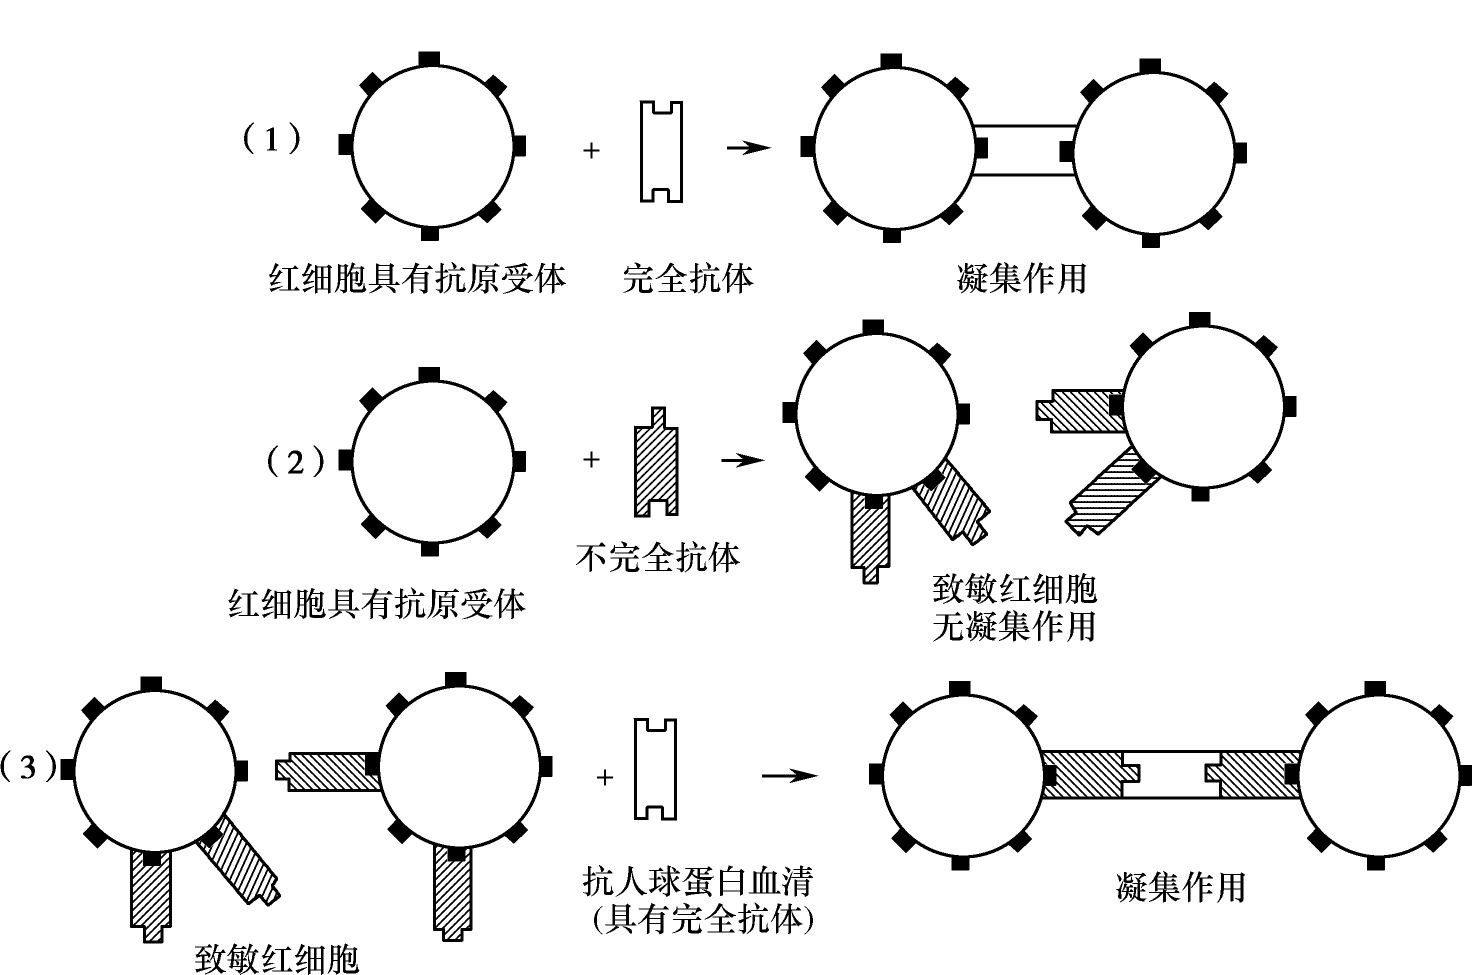
\includegraphics[width=5.09375in,height=3.32292in]{./images/Image00178.jpg}
 \captionsetup{justification=centering}
 \caption{抗人球蛋白试验反应示意图}
 \label{fig33-4}
  \end{figure} 

(1)完全抗体可使具有抗原受体的红细胞发生凝集作用;
(2)不完全抗体使红细胞致敏,但无凝集作用;
(3)加入抗人球蛋白血清后,可使致敏红细胞发生凝集作用

\begin{figure}[!htbp]
 \centering
 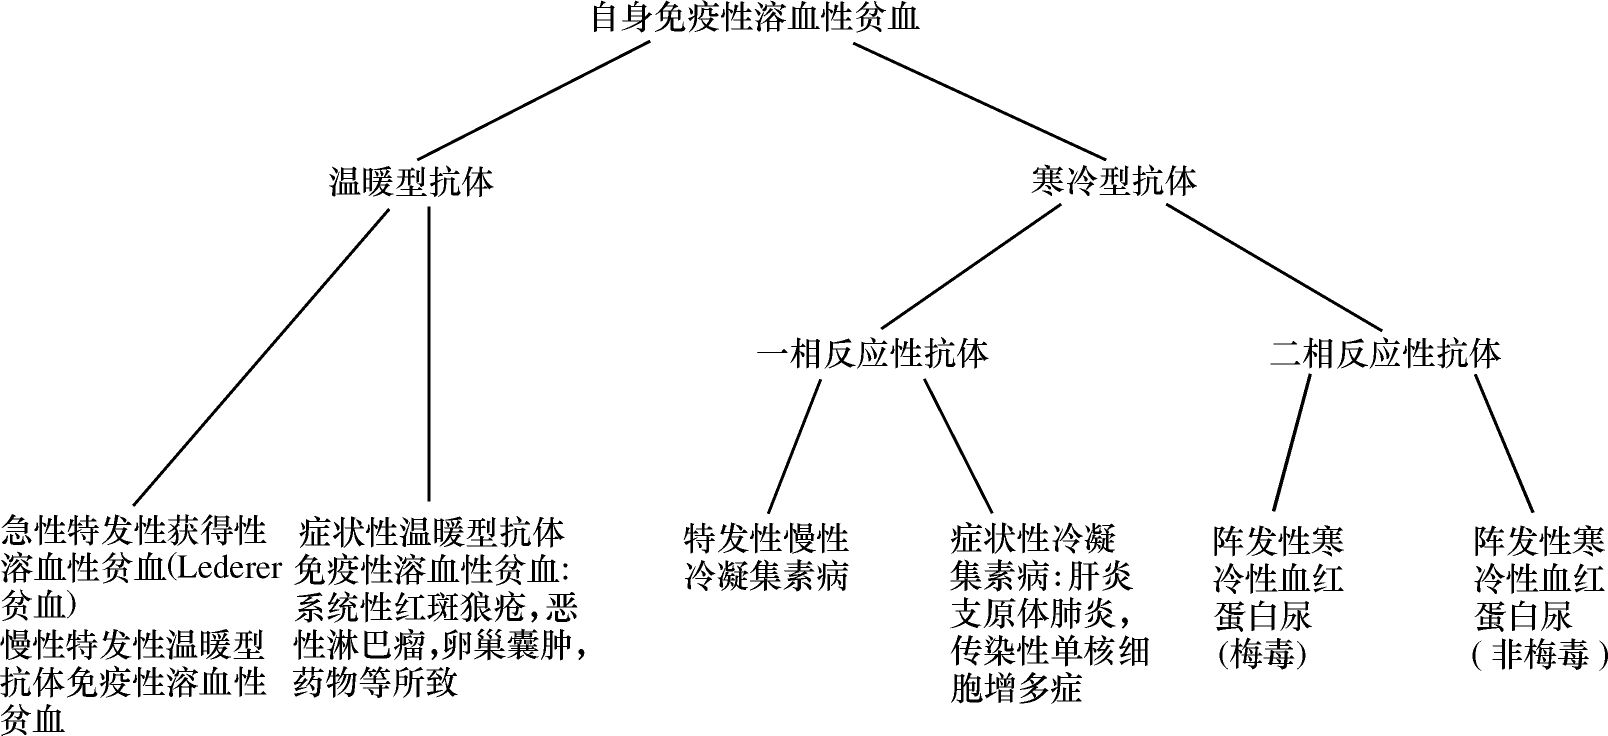
\includegraphics[width=5.5625in,height=2.53125in]{./images/Image00179.jpg}
 \captionsetup{justification=centering}
 \caption{自身免疫性溶血性贫血分类}
 \label{fig33-5}
  \end{figure} 

\subparagraph{(一)温抗体性自身免疫性溶血性贫血}

\hypertarget{text00260.htmlux5cux23CHP33-5-4-1-1-1-1}{}
1.急性特发性获得性溶血性贫血

本病又名Lederer贫血,是一种少见的原因未明的特发性急性溶血性贫血,患者多为小儿。严重的溶血性贫血、发热、血培养及其他检查除外感染的存在及输血有良效时,提示本病的诊断。

本病的诊断根据是:①起病急骤,具有急性溶血性贫血的临床表现;②周围血液中白细胞数增多;③部分病例直接抗人球蛋白试验阳性;④部分病例有温暖型自身凝集素和温暖型自身溶血素;⑤输血治疗有良好效果。此病应与慢性特发性温抗体性免疫性溶血性贫血相区别,根据前者多见于小儿,病情急重,抗人球蛋白试验不一定呈阳性,且输血有良好的效果,可与后者相区别。

\hypertarget{text00260.htmlux5cux23CHP33-5-4-1-1-1-2}{}
2.原发性温抗体性自身免疫性溶血性贫血

为原因未明的自身免疫性溶血。机体可能在B细胞克隆受到激活、T细胞亚群失调导致辅助性T细胞活化、或红细胞表面抗原性改变等原因下,引起自身抗体的产生。溶血主要发生于血管外,红细胞经吸附自身不完全抗体或补体而致敏,抗体不能使红细胞直接发生凝集,但其Fc段部分暴露于红细胞膜上,当红细胞经过肝窦和脾窦时,被巨噬细胞的Fc受体所识别,导致抗体与部分红细胞膜被吞噬消化。红细胞膜内蛋白质及磷脂物质的丧失,使得红细胞形态趋于球形,难于通过脾窦而遭到破坏。如用含有抗凝剂的血标本作血常规检查时,发现明显的红细胞凝集颗粒,加温后不能防止,则提示本病诊断的可能性。

本病呈慢性起病,病史多年。患者感全身不适、乏力,体检发现贫血、黄疸与肝脾大。慢性经过中常有急性发作。网织红细胞计数与血清黄疸指数测定为估计溶血程度的良好指标。有些急重病例,可有血红蛋白尿出现。肾上腺皮质激素治疗有良效。

本病的实验室检查特点是:①贫血为正常细胞、正常色素性,程度轻重不一;②外周血片可见多量球形红细胞,及有核红细胞,网织红细胞比例增高;③多数病例直接抗人球蛋白试验呈阳性,间接抗人球蛋白试验多呈阴性;主要抗体为IgG,同时具有IgG和C3者较多见;④极少数病例有温性自身溶血素,主要为IgM,体外可使酶处理的红细胞直接溶解;⑤红细胞脆性试验正常(仅在急性发作时脆性增高);⑥康氏或华氏反应可呈假阳性反应(因患者血清中同时存有抗类脂质抗体)。

本病的诊断依据:对获得性溶血性贫血患者,直接抗人球蛋白试验阳性,为IgG和(或)C3型,4个月内无输血或特殊药物史,结合临床表现,可考虑温抗体性自身免疫性溶血性贫血。

抗人球蛋白试验对本病的诊断有重要意义。抗人球蛋白试验方法近年有了发展,大多数病例用抗免疫球蛋白G特异性(anti-IgG
specificity)的抗人球蛋白血清作直接Coombs试验,呈阳性反应。用抗补体特异性(anti-complement
specificity)的抗人球蛋白血清作直接Coombs试验,也呈阳性反应(红细胞表面有补体成分序贯被覆)。必须指出,少数患者直接Coombs试验可呈阴性,此时可选用高效价的抗人球蛋白血清定期作直接Coombs试验,可获阳性结果。文献报道在这些直接Coombs试验阴性的患者血浆中检出温性溶血素,对诊断也有帮助。

对抗人球蛋白试验应有正确的估价。抗人球蛋白试验一般在原发性红细胞结构异常所致的溶血性贫血时为阴性,而在后天性免疫性溶血性贫血时为阳性。在各类型获得性非免疫性溶血性贫血时,则此试验为阴性。但当出现以下情况时,Coombs试验可呈假阴性:①红细胞未洗涤充分,使得血清残存的非温抗体类球蛋白中和了抗人球蛋白;②红细胞膜上结合的温抗体数较少;③某些温抗体与红细胞亲和力低,洗涤时脱落。以下情况则会导致Coombs假阳性:①正常人在感染时可导致红细胞被C3致敏;②某些疾病如PNH、肾炎使得体内C3水平升高;③红细胞C3受体结合了免疫复合物。

患者酸化血清试验(Ham)偶可呈阳性,须注意与阵发性睡眠性血红蛋白尿相区别(参见第113.2.2节)。本病偶尔临床上有被误诊为遗传性球形红细胞增多症者。本病除缺乏遗传因素和发病年龄较迟外,红细胞脆性试验的动态观察为重要鉴别诊断依据。

本病红细胞的凝集作用,往往使配血发生困难,有因此而误诊AB型或Rh阳性血型者,有怀疑时可将患者红细胞洗涤处理后再作配血试验,可防止发生这种错误。

\hypertarget{text00260.htmlux5cux23CHP33-5-4-1-1-1-3}{}
3.继发性温抗体性自身免疫性溶血性贫血

据报道,自身免疫性溶血性贫血大约40\%~60\%可以找到明确病因,为继发性。

肿瘤性疾病(白血病、恶性淋巴瘤、多发性骨髓瘤、卵巢囊肿、某些实体瘤等)、自身免疫性疾病(系统性红斑狼疮、类风湿关节炎、溃疡性结肠炎、自身免疫性甲状腺炎等)及感染(传染性单核细胞增多症、病毒性肝炎、结核病等)均可引起溶血性贫血。最常见诱发AIHA的药物是嘌呤核苷酸类似药,主要包括氟达拉滨和克拉屈滨,几乎均为温抗体型AIHA,多数见于慢性淋巴细胞白血病治疗中,发生率为5\%~22\%;另一种常可引起AIHA的药物是干扰素,见于丙型病毒性肝炎、慢性粒细胞白血病、肾癌长期干扰素治疗中。也有报告由于奎宁、乙酰非那西丁、非那西丁、对氨基水杨酸、大量青霉素、甲基多巴等药物所引起。本病的临床和实验室检查所见,与原发性温抗体性自身免疫性溶血性贫血相似,两者抗人球蛋白试验均呈阳性,但本病同时有原发病作为发病的基础。

\subparagraph{(二)冷抗体型自身免疫性溶血性贫血}

最适反应温度在30℃以下的自身红细胞抗体为冷抗体,由冷抗体引起的溶血性贫血称为冷抗体型AIHA。

\hypertarget{text00260.htmlux5cux23CHP33-5-4-1-1-2-1}{}
1.慢性原发性冷凝集素综合征

本病又名可逆性低温冷凝集素症所致的慢性溶血性贫血,临床上少见,伴血红蛋白尿则更少。本病多见于中年人及老年人。

患者冷凝集素效价比正常人的冷凝素效价明显增高,这种冷凝集素是免疫球蛋白M
(18M),含有单一类型的轻链,为单克隆(monoclone)B细胞所产生。高效价的冷凝集素在低温时有凝集自身红细胞的作用,成堆的红细胞可阻塞周围毛细血管,红细胞也因而破裂。患者受寒诱发溶血性贫血伴有血红蛋白尿及手足发绀和肢端疼痛(雷诺现象),提示本病诊断的可能性。血清冷凝集素效价增高则可确诊。

本病因寒冷诱发症状,须与阵发性寒冷性血红蛋白尿相区别(见下文“3”部分)。本病直接抗人球蛋白试验阳性,应与温抗体性自身免疫性溶血性贫血相鉴别。后者溶血程度较重,发病与寒冷无关,用抗IgG的或抗补体的抗人球蛋白血清作直接Coombs试验呈阳性反应。在慢性冷凝集素综合征,溶血程度较轻,发病与寒冷关系密切,用抗IgG的或抗IgM的抗人球蛋白血清作直接Coombs试验呈阴性反应,用抗补体C3或C4的抗人球蛋白血清作直接Coombs试验则呈阳性反应。

\hypertarget{text00260.htmlux5cux23CHP33-5-4-1-1-2-2}{}
2.急性冷凝集素综合征

为冷凝集素效价增高所致的急性溶血性贫血,常见于肺炎支原体肺炎(原发性非典型肺炎)及传染性单核细胞增多症,此外也可发生于巨细胞病毒感染、梅毒、盘状红斑狼疮、锥虫病、螺旋体病、重症贫血、疟疾、多发性骨髓瘤和肝硬化等。实验室检查结果与慢性原发性冷凝集素综合征基本相同,即冷凝集素效价明显增高,效价可高至1∶1000,甚至1∶16
000(正常人<1∶64)。

肺炎支原体肺炎合并溶血常出现在病程的第三周,发生于肺炎的恢复期,正当冷凝集素的效价处于高峰阶段,也有少数在肺炎急性起病时发作。溶血多为自限性,常持续1~3周。其效价增高的冷抗体是抗I凝集素。这种冷抗体也是一种免疫球蛋白M(IgM),它含有两种类型的轻链,因此提示来源于多克隆(polyclone),可作为与慢性原发性冷凝集素综合征相区别的参考。

传染性单核细胞增多症合并溶血时,溶血多与原发病同时出现。溶血发生时往往突然体温升高,有重度贫血,肢端发绀。效价增高的冷抗体是抗Ⅰ凝集素,而不同于慢性原发性冷凝集素综合征和肺炎支原体肺炎的抗Ⅰ凝集素的冷抗体。

\hypertarget{text00260.htmlux5cux23CHP33-5-4-1-1-2-3}{}
3.阵发性寒冷性血红蛋白尿

本病是在全身或局部(手泡在冷水中或进食冷饮料)受冷后,突然出现的以血红蛋白尿为特征的少见的急性溶血性疾病。本病多与先天或后天梅毒感染有关,也有少数非梅毒所致的病例报告,如水痘、传染性单核细胞增多症、支原体肺炎等。本病的抗体(D-L抗体或称冷热抗体)为寒冷型抗体IgG,而不同于温暖型抗体IgG。前者所导致的溶血主要为血管内,当患者受冷后,流经皮肤毛细血管的红细胞(一般在20℃以下)即与D-L抗体结合,随之抗体结构发生变异,使其补体结合位点暴露,从而激活系列补体,形成膜攻击复合物,破坏红细胞,导致溶血。

冷热溶血试验(D-L试验)对诊断本病有重要意义。此试验的原理是:D-L抗体系非凝集素性IgG,仅在寒冷条件下(冷相)结合红细胞,而在正常体温时(热相)分解消失。如果存在补体,被抗体致敏的红细胞则发生溶解。D-L试验时将患者血清与正常人红细胞在4℃孵育,然后加入鼠血清或与患者红细胞血型相配的血清,以供应补体,在加热至37℃即可观察到溶血的发生。

阵发性寒冷性血红蛋白尿的诊断根据为:①受冷后有棕黑色尿发作史,化验证明为血红蛋白尿;②D-L试验阳性;③血清梅毒反应与Rosenbach试验阳性。

无论患者有无感染梅毒,华氏反应几乎均可呈阳性,但在梅毒病例发作后,华氏反应却可转为阴性(由于介体的消耗)。对有怀疑的病例,则需隔数天后复查,因此追查梅毒病史相当重要。在非梅毒病例,华氏反应仅呈假阳性,可用螺旋体制动试验区别之。

本病直接抗人球蛋白试验呈阳性反应,可能是由于二相反应性抗体能固定补体成分,使补体被覆红细胞表面,因而用含有抗补体的抗人球蛋白血清作直接抗人球蛋白试验呈阳性。如用仅含有抗IgG的抗人球蛋白血清作直接抗人球蛋白试验,则呈阴性,借此可与慢性特发性温暖型抗体免疫性溶血性贫血相区别。当-蓝试验为更重要的鉴别诊断试验。

与阵发性寒冷性血红蛋白尿极易混淆的是阵发性睡眠性血红蛋白尿(PNH),因前者溶血乃由IgG结合补体所致,故可出现酸溶血试验和蔗糖溶血试验阳性,很像PNH。但PNH患者没有D-L抗体,阵发性寒冷性血红蛋白尿患者没有PNH细胞(缺乏CD55、CD59等GPI锚接蛋白的细胞),借此可鉴别之。

本病尚需与特发性慢性冷凝集素病所致血红蛋白尿相鉴别(参见上文“(二)”部分)。

\paragraph{二、同种免疫性溶血性贫血}

同种免疫抗体不作用于自身的红细胞,而仅作用于异体的红细胞,此为与自身免疫抗体不同之点。此型溶血性贫血常发生于:①ABO血型不合溶血性输血反应;②Rh血型不合溶血性输血反应;③新生儿ABO溶血病与新生儿Rh溶血病。

\subparagraph{(一)ABO血型不合溶血性输血反应}

ABO血型不合溶血性输血反应原因有二:①供血者红细胞溶血。最多由于ABO血型不合所致;有些AB型受血者血浆中含有不规则抗体,也可使供血者红细胞溶血。②受血者红细胞溶血。临床常见以下情况:将A型血错输给B型或O型血患者,或将B型血错输给A型或O型血患者,多由于配血或输血错误引起,是最常见的溶血反应原因。另外,以前认为O型血为“万能给血者”,可把O型血输给任何非O型血患者,但其实因30\%~40\%的O型人血浆中含有免疫性抗A及抗B抗体,若效价高则不能被可溶性血型物质中和。把这种O型全血输给A、B或AB型患者后,供者血浆内的抗A及抗B抗体则可破坏受血者的红细胞而发生溶血。因此,除非在万分紧急而又无同型血的情况下,不应将O型全血输给其他血型患者。

由于ABO血型抗体是IgM型天然完全抗体,其在生理盐水中可与具有相应抗原的红细胞直接发生凝集,故血型不合,首次输血即可发生输血反应。ABO血型不合溶血性输血反应的溶血多属血管内溶血,其典型临床表现为:输入少量血液后,患者突然发生剧烈腰痛、寒战、高热、恶心、呕吐,甚至苍白、大汗、脉细弱、血压下降等休克症状;酱油样小便;反应严重者可发生急性肾衰竭;少数患者可有出血倾向,表现为伤口出血、手术野渗血不止等。从开始输血到出现症状,时间长短不一,取决于抗体效价,输入血量和溶血速度。若凝集素效价高,输入10~15ml即可产生症状。

偶尔溶血反应轻微,可无症状;仅在输血后血红蛋白量达不到预期上升水平,或在输血150mL后一周内血红蛋白量比输血前的水平更低。

疑有溶血反应,应立即停止输血,并按下列方法进行诊断:①重作血型鉴定及配血试验;②取患者血液离心沉淀后观察血浆内有无游离血红蛋白;③血红蛋白尿检查(取反应后第一次尿);④取患者血作直接及间接抗人球蛋白试验;⑤取患者血清作黄疸指数、胆红素定性与定量测定(反应后3~6小时取血);⑥如有需要,可对少见的血型抗体进行测定;⑦输血瓶内血液细菌学检查。

血型不合的输血所致溶血反应与其他输血反应的特点参考表\ref{tab33-8}。

\begin{table}[htbp]
\centering
\caption{各种输血反应的特点}
\label{tab33-8}
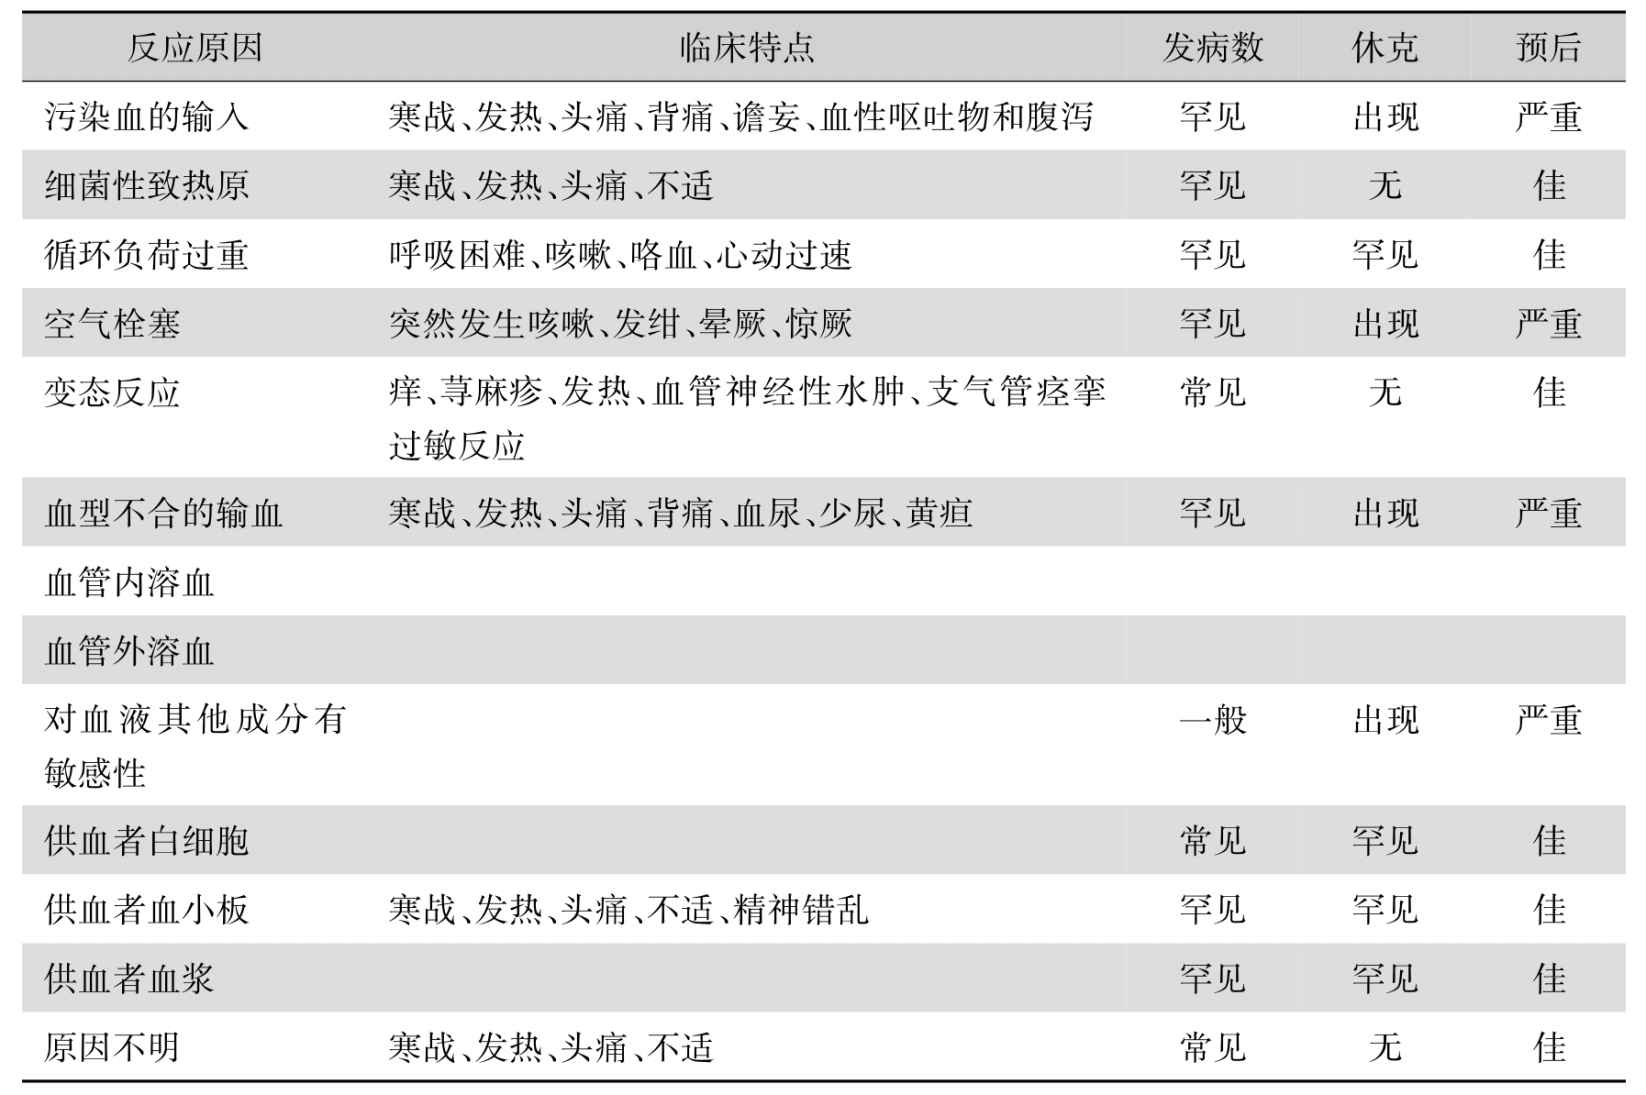
\includegraphics[width=5.96875in,height=3.96875in]{./images/Image00180.jpg}
\end{table}

\subparagraph{(二)Rh血型不合溶血性输血反应}

Rh系统血型共有6个抗原,即C、D、E、c、d、e,它们的抗原性强弱依次为D>E>C>c>e>d,D抗原的抗原性最强,是引起Rh血型不合溶血反应的主要抗原。临床上通常将含有D抗原的红细胞通称为Rh阳性,无D抗原者称为Rh阴性。我国人Rh阴性的百分率甚低,综合文献报道约平均为0.9\%,是以因Rh因子所致的输血意外较少见。但我国少数民族Rh阴性的百分率却较高,有人曾在贵州省某些地区,发现苗族居民的Rh阴性的百分率为29.4\%。输血事故虽多由Rh(D)抗原引起,但近年由于Rh血型系统的其他抗原,如抗E和抗C抗体引起的输血反应也有报道。

Rh阴性人的血浆内并无相应的抗Rh抗体,但当有下列情况之一时则有抗Rh抗体(多为不完全抗体)形成:①输入Rh阳性的红细胞后;②女性妊娠Rh阳性的胎儿时。

如将Rh阳性的血液输给上述Rh阴性致敏的人,则抗原(存在于供血者红细胞内)与抗体(存在于受血者血浆内)相结合,使输入的红细胞发生溶血。红细胞主要在单核-吞噬细胞系统内破坏,即所谓血管外溶血。曾接受多次输血的人或孕妇因输血而发生溶血现象时,应考虑此种情况的可能性。可用Rh血型鉴定及直接或间接抗人球蛋白试验证明之。

\subparagraph{(三)新生儿溶血病}

是由于孕妇与胎儿血型不合,母体产生了与胎儿红细胞血型抗原相对应的抗体,经胎盘进入胎儿体内而引起溶血的一组疾病。

新生儿周围血涂片出现众多的有核红细胞(有核红细胞与白细胞的比例达10∶100),提示本病的可能性。此外,败血症、先天性心脏病、早产婴及早产婴核黄疸等也可有周围血有核红细胞增多,须注意鉴别。新生儿溶血病的黄疸尚需与其他疾病所致新生儿黄疸相区别。前者一般出现于生后24小时以内,而新生儿生理性黄疸和感染性黄疸的出现时间较迟,在鉴别诊断上有一定意义。先天性胆道畸形所致阻塞性黄疸于出生后2~3周起病,以阻塞性黄疸为主,并无贫血,有助于与本病相鉴别。新生儿溶血病的母亲分娩史中多有前胎次婴儿发生黄疸的病史(Rh不合者常见于第3、4胎;ABO不合者常见于第一胎),母血中检出不完全抗体等对鉴别诊断也甚有帮助。

新生儿溶血病通常分为新生儿Rh溶血病和新生儿ABO溶血病两种:

\hypertarget{text00260.htmlux5cux23CHP33-5-4-1-2-3-1}{}
1.新生儿Rh溶血病

Rh溶血病时,胎儿具有孕母所缺乏的Rh抗原,当胎儿血液有机会通过胎盘进入母体,经过8~9周或6个月的时间,孕妇产生同种免疫。该妇女如再次怀孕具有相同抗原的胎儿时,孕母即产生大量抗胎儿红细胞的IgG抗体,经胎盘进入胎儿,导致溶血的发生。本病以水肿、黄疸、贫血、肝脾大及血液中出现众多的有核红细胞为特征。国内有少数病例报告。

新生儿Rh溶血病的产生需要有下列四个条件:

(1)父为Rh阳性,母为Rh阴性,胎儿为Rh阳性。

(2)母血含有抗Rh抗体。

(3)母血中的抗Rh抗体必须流入胎儿血循环中。

(4)母血中的抗Rh抗体作用于胎儿的红细胞使之破坏。

新生儿出生24小时内出现黄疸且迅速加重,实验室检查母亲和新生儿Rh血型不同(母Rh阴性,新生儿Rh阳性),强烈提示本病的诊断。

新生儿Rh溶血病的诊断主要根据下列的实验室检查:①患儿血型为Rh阳性,母亲为Rh阴性;②患儿红细胞直接抗人球蛋白试验阳性,表明患儿的红细胞与免疫抗体结合,对新生儿Rh溶血病的诊断具有重要意义;③产妇血清与其丈夫或患儿红细胞作木瓜酶试验、间接抗人球蛋白试验、胶体介质试验均呈阳性。如产妇与其丈夫或患儿ABO血型不合,作以上试验前,应先用特异性血型物质中和产妇血清中的天然抗A或抗B抗体。上述任一试验结果阳性,均表明产妇血清中含有与其丈夫或患儿红细胞血型抗原相应的免疫抗体,诊断即可确立;④还可进一步用一套标准抗原红细胞,检测产妇体内抗体的特异性。

\hypertarget{text00260.htmlux5cux23CHP33-5-4-1-2-3-2}{}
2.新生儿ABO溶血病

新生儿ABO溶血病较Rh溶血病多见,与母亲、婴儿ABO血型不同有关。母亲血液中含有免疫性抗A或抗B抗体,它通过胎盘作用于胎儿的A或B型红细胞而引起溶血。新生儿ABO溶血病中,母亲为O型,新生儿为A或B型者占90\%以上,而极少见患儿与A或B型的母亲血型不合导致的溶血。由于大多数母体并无产生抗A或抗B免疫抗体的能力,所以虽然我国汉族母婴ABO血型不合妊娠达26.9\%,新生儿ABO溶血病仅占极少数。新生儿红细胞膜上的A和B抗原位点较少,因此能结合的免疫抗体也不多,ABO溶血病一般较轻。患儿黄疸多于出生后2天内出现,5天时达高峰,以后即迅速消退,且大多除黄疸外无其他症状。

新生儿黄疸而母亲和新生儿的血型不同(通常母亲为O型而新生儿为A或B型),强烈提示本病的可能性。

以下试验有助于新生儿ABO溶血病的诊断:①患儿红细胞直接抗人球蛋白试验阳性(必须指出,以惯用的抗人球蛋白血清作试验极少阳性,而用有较高效价的抗人球蛋白血清,则60\%~70\%病例可呈阳性)。②产妇血清先用特异性血型物质将天然抗A或抗B抗体中和,然后与其丈夫或患儿红细胞作木瓜酶试验、间接抗人球蛋白试验及胶体介质试验均阳性。③产妇溶血素试验阳性(1∶8以上)。

\paragraph{三、药物诱发的免疫性溶血性贫血}

本病的致病机制为药物或其代谢产物与红细胞膜成分发生作用,疏松或紧密结合后,导致新抗原的形成,引起免疫性溶血。

按其引起溶血的机制,可分为以下三类:

\subparagraph{(1)免疫复合物型:}

对氨基水杨酸、异烟肼、利福平、奎宁、非那西丁等属于此类。药物作为半抗原,与血清蛋白质结合形成抗原,刺激机体产生抗体。若重复应用该药物,则导致药物-抗体免疫复合物形成,吸附于红细胞膜上并直接激活补体,破坏红细胞。其临床特点为:①过去有服药史,引起溶血的药量常很少;②起病急,病情较重;③溶血常为血管内,补体直接导致溶血;④停用药物,溶血迅速好转;⑤直接抗人球蛋白试验阳性,间接试验阴性。

\subparagraph{(2)半抗原型:}

青霉素、氨苄西林、甲氧西林等属此类。药物作为半抗原与红细胞膜及血清内蛋白质形成全抗原,所产生的抗原与吸附在红细胞膜上的药物发生反应,导致红细胞破坏。其特点为:①通常诱发溶血的药物为超大剂量应用;②起病稍快但非急性;③溶血方式为血管外,脾阻留红细胞导致其破坏;④停药后病情常持续几天至几星期;⑤直接抗人球蛋白试验阳性,间接试验阴性。

\subparagraph{(3)自身抗体型:}

代表药物为甲基多巴、左旋多巴等。此类药物结合红细胞,改变红细胞的抗原性而致溶血。其临床特点是:①一般长期用药致病;②起病慢,发生轻度溶血;③溶血主要为血管外,脾脏阻留致敏红细胞而使之破坏;④停药后溶血可持续6个月至1年,甚至更长;⑤直接及间接抗人球蛋白试验均可阳性。该型临床表现与原发性AIHA甚难区分。

凡出现自身免疫性溶血性贫血者,均应仔细询问病史,有肯定服用上述药物史者,诊断一般不难,实验室检查可肯定溶血性质及与药物之间的关系。

\subsubsection{113.2.2 非免疫性溶血性贫血}

此类溶血性贫血与免疫机制及遗传因素关系不大,溶血多由于药物、化学药品或细菌毒素直接作用于红细胞所引起。

\paragraph{一、化学物品及某些药物所致溶血性贫血}

某些药物及化学物品可引起溶血。症状发生的缓急与中毒轻重及机体反应性等因素有关。黄疸在溶血发生后迅速出现,血红蛋白尿只见于重症病例,某些病例可伴有发绀,此乃由于高铁血红蛋白血症所致。

引起溶血的药物及化学物品可分为三类:①直接损害红细胞的药物及化学物品:如砷、砷化氢、苯、硝基苯、苯胺及铅等,引起溶血的剂量较大。此类溶血起病较慢,红细胞有海涅茨小体形成。②损害缺乏G6PD的红细胞的药物(参见第103.1.3节)。③某些药物通过免疫作用损害红细胞,如奎宁、奎尼丁及非那西丁等,直接抗人球蛋白试验可检出温暖型抗体(参见第103.1.3节)。

诊断的主要根据为:①有关的药物及化学物品接触史;②急性血管内溶血的临床表现;③红细胞有海涅茨小体形成;④高铁血红蛋白还原试验还原速率减慢。

\paragraph{二、感染性溶血性贫血}

此类贫血可见于疟疾(疟原虫在红细胞内繁殖导致红细胞破裂),黑热病(参见第120节)、病毒感染、败血性细菌感染(如产气荚膜梭菌、溶血性链球菌、葡萄球菌、大肠杆菌、伤寒杆菌)等。

某些感染所致溶血性贫血,可能与患者红细胞缺乏G6PD有关。

由感染导致的溶血,通常在原发病得到迅速有效的控制后,血液学异常可完全恢复。

\paragraph{三、脾大性溶血性贫血}

本病大都有明显的脾大。溶血并非由于原发性红细胞结构异常而被脾脏所破坏,也不是由于机体产生自身免疫抗体,而是因为脾脏处理衰老的红细胞和异常红细胞的场所,起过滤和处置作用。当脾大时,红细胞在脾索中行进时间长,有更多机会接触周围的吞噬细胞,某些变形性低的老化红细胞更易在脾索中受阻,而遭到破坏。脾大患者在一周内需两次输血,提示有溶血发生的可能。化验检查可发现粪胆原排量增多,周围血网织红细胞增多,骨髓中红细胞系统增生旺盛。脾大的原因为:慢性白血病、恶性淋巴瘤、骨髓纤维化、结节病、戈谢病及门脉高压症等。

\paragraph{四、阵发性睡眠性血红蛋白尿(PNH)}

阵发性睡眠性血红蛋白尿是一种获得性造血干细胞克隆缺陷性疾病,其血细胞(红细胞、粒细胞及血小板)膜对补体异常敏感而被破坏,导致持续性血管内溶血,常有阵发性、睡眠后血红蛋白尿发作,全血细胞减少。本病在国内并非少见,患者多为男性青壮年,起病大多徐缓,但少数也可较急。轻型病例可无血红蛋白尿发作,仅长期有慢性溶血的表现。

由于分子克隆技术的开展,目前已经明确本病是由于造血干细胞发生X染色体上PIG-A基因突变,导致PNH异常血细胞的细胞膜上缺乏糖肌醇磷脂连接蛋白(GPI连接蛋白),引起细胞功能的改变。其中较显著的变化是细胞对补体敏感性增加,导致溶血和全血细胞减少。

针对PNH红细胞对补体敏感及缺少GPI连接蛋白的有以下试验,对诊断有重要意义。①蔗糖溶血试验:PNH异常细胞在等渗低离子强度的溶液中更易遭到补体破坏。本试验敏感性高,但特异性较差,容易出现假阳性,常作为诊断本病的初筛试验。②酸化血清溶血试验(Ham试验):补体在酸性条件下活性增高,因此PNH病态红细胞在pH
6.4时更易遭到破坏,而正常细胞则不会。本实验特异性较强,通常作为诊断PNH的主要依据。③蛇毒因子溶血试验:蛇毒本身没有溶血作用,但可在血清成分的协同下通过替代途径激活补体,导致PNH细胞溶解。本试验特异性及敏感性均高。④补体溶血敏感试验:用冷凝集素和抗人红细胞抗体致敏红细胞,通过经典途径激活补体,观察能使红细胞溶解所需要的补体量,判断红细胞对补体的敏感性。⑤PNH异常血细胞的检测:衰变加速因子(CD55)和膜攻击复合物攻击因子(CD59)作为GPI连接蛋白,存在于所有系列的血细胞上,且与临床表现关系密切。以流式细胞仪,利用CD55、CD59单抗检测PNH患者外周血细胞,可发现CD55\textsuperscript{-}
、CD59\textsuperscript{-}
细胞的比例明显高于正常人。本实验是目前诊断本病最特异、最敏感且可定量的方法。

PNH的诊断标准:①临床表现符合PNH;②上述实验室检查中有两项以上阳性;或只有一项阳性但结果可靠,并有血管内溶血的证据,能除外其他溶血性贫血者。符合以上条件即可确诊。

国内作者回顾性分析76例PNH患者的临床资料,60.5\%患者以溶血为主要表现,21.1\%以骨髓衰竭为主要表现,18.4\%以血栓形成为主要表现。其中2例进展为骨髓增生异常综合征/急性髓系白血病。该病临床表现多样,延诊或误诊者颇多。因此建议对原因不明的贫血需注意本病的可能,Ham试验阴性亦不能除外本病,须综合全面检查材料甚至长期密切随诊以落实诊断。

PNH应注意与以下疾病鉴别:

\subparagraph{1.再生障碍性贫血(AA)}

由于PNH的细胞膜缺陷涉及各系血细胞,因此常有外周血三系减少,易与AA相混淆。不同的是典型的PNH骨髓造血多活跃(特别是红系),有溶血的表现,酸溶血、蛇毒因子溶血试验多阳性,可检出PNH细胞。AA则骨髓增生减低,非造血细胞增多,网织红细胞百分率和绝对值常显著降低,无溶血表现。若骨髓增生减低而又能查出类似PNH的异常红细胞,或是有PNH的临床及实验室所见但骨髓增生低下者,应怀疑是否有疾病的转化或是兼有两病。

\subparagraph{2.骨髓增生异常综合征(MDS)}

少数PNH患者骨髓象可有病态造血现象,骨髓原始粒细胞比例轻度增加,甚至在外周血见到原始粒细胞,但通常为一过性,可以自行消失。但极个别的患者会经过数年后转化为MDS。

\subparagraph{3.缺铁性贫血(IDA)}

PNH因长期血管内溶血,产生血红蛋白尿而致失铁,但不同的是,本病经补铁后不能使贫血完全纠正,大量补铁反而会加重溶血的发生。

目前发现,PNH与AA、MDS、急性白血病及骨髓纤维化关系密切。原有肯定的PNH而后转化为AA,而原有的PNH的表现包括实验室检查已不存在;或原有明确的AA其后转化为PNH,AA的表现消失:或PNH伴有AA特征,AA伴有PNH特征,通称为PNH-AA综合征。PNH亦可经过数年转化为MDS;一些骨髓纤维化的患者并发PNH;一些AA、PNH及骨髓纤维化患者,可能发展为急性白血病。因此,在诊断PNH时,要注意患者可能合并存在另一些血液系统疾病,以及PNH可能发展为另一种血液疾病。上述四种关系密切的疾病,可能由于都是造血干细胞克隆性疾病的结果。

必须指出,酸化血清试验对诊断阵发性睡眠性血红蛋白尿有特异性,但在下述两种少见的情况下,酸化血清试验也呈阳性:①先天性或后天性溶血性贫血,当其红细胞呈明显球形时;②某些自身免疫性溶血性贫血(热溶血素或冷凝集素所致者)。下述两项试验对鉴别诊断有意义:①患者红细胞加酸化正常血清(试验前加热灭活),如发生溶血见于球形红细胞增多症,无溶血发生见于阵发性睡眠性血红蛋白尿及自身免疫性溶血性贫血;②正常红细胞加患者酸化血清,溶血发生在自身免疫性溶血性贫血而不发生在阵发性睡眠性血红蛋白尿。少数PNH病例,直接抗人球蛋白试验也可呈阳性,但根据上述两个试验结果及红细胞寿命测定(表\ref{tab33-9}\footnote{*包括温暖型抗体自身免疫性溶血性贫血及冷凝集素病}),不难与各型自身免疫性溶血性贫血相鉴别。近年文献报道一些先天性红细胞生成异常性贫血Ⅱ型(congenital
dyserythropoietic anemia
typeⅡ),酸化血清试验也呈阳性,但这种病例以骨髓有核红细胞含有多个细胞核为特征。

\begin{longtable}{c}
 \caption{5种溶血性贫血鉴别诊断}
 \label{tab33-9}
 \endfirsthead
 \caption[]{5种溶血性贫血鉴别诊断}
 \endhead
 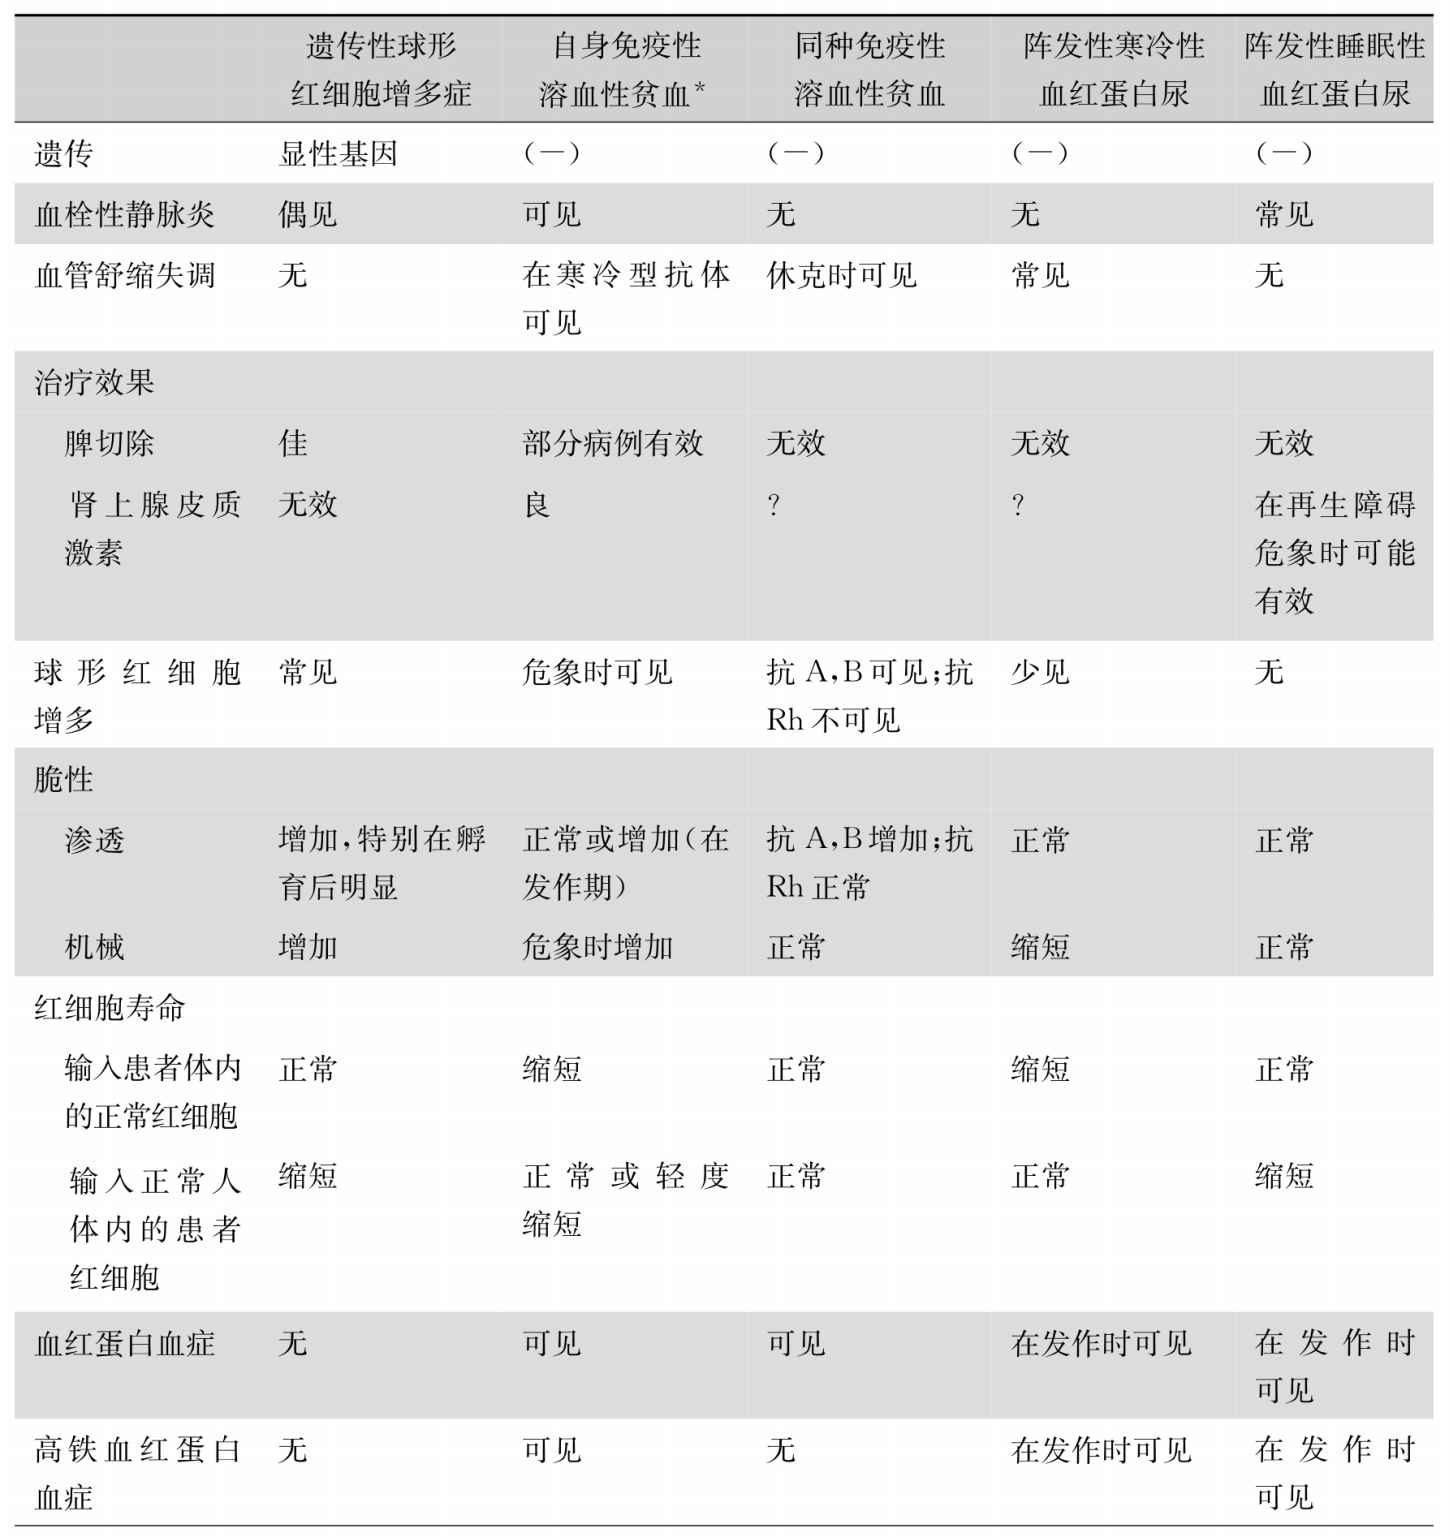
\includegraphics[width=\textwidth,height=\textheight,keepaspectratio]{./images/Image00181.jpg}\\
 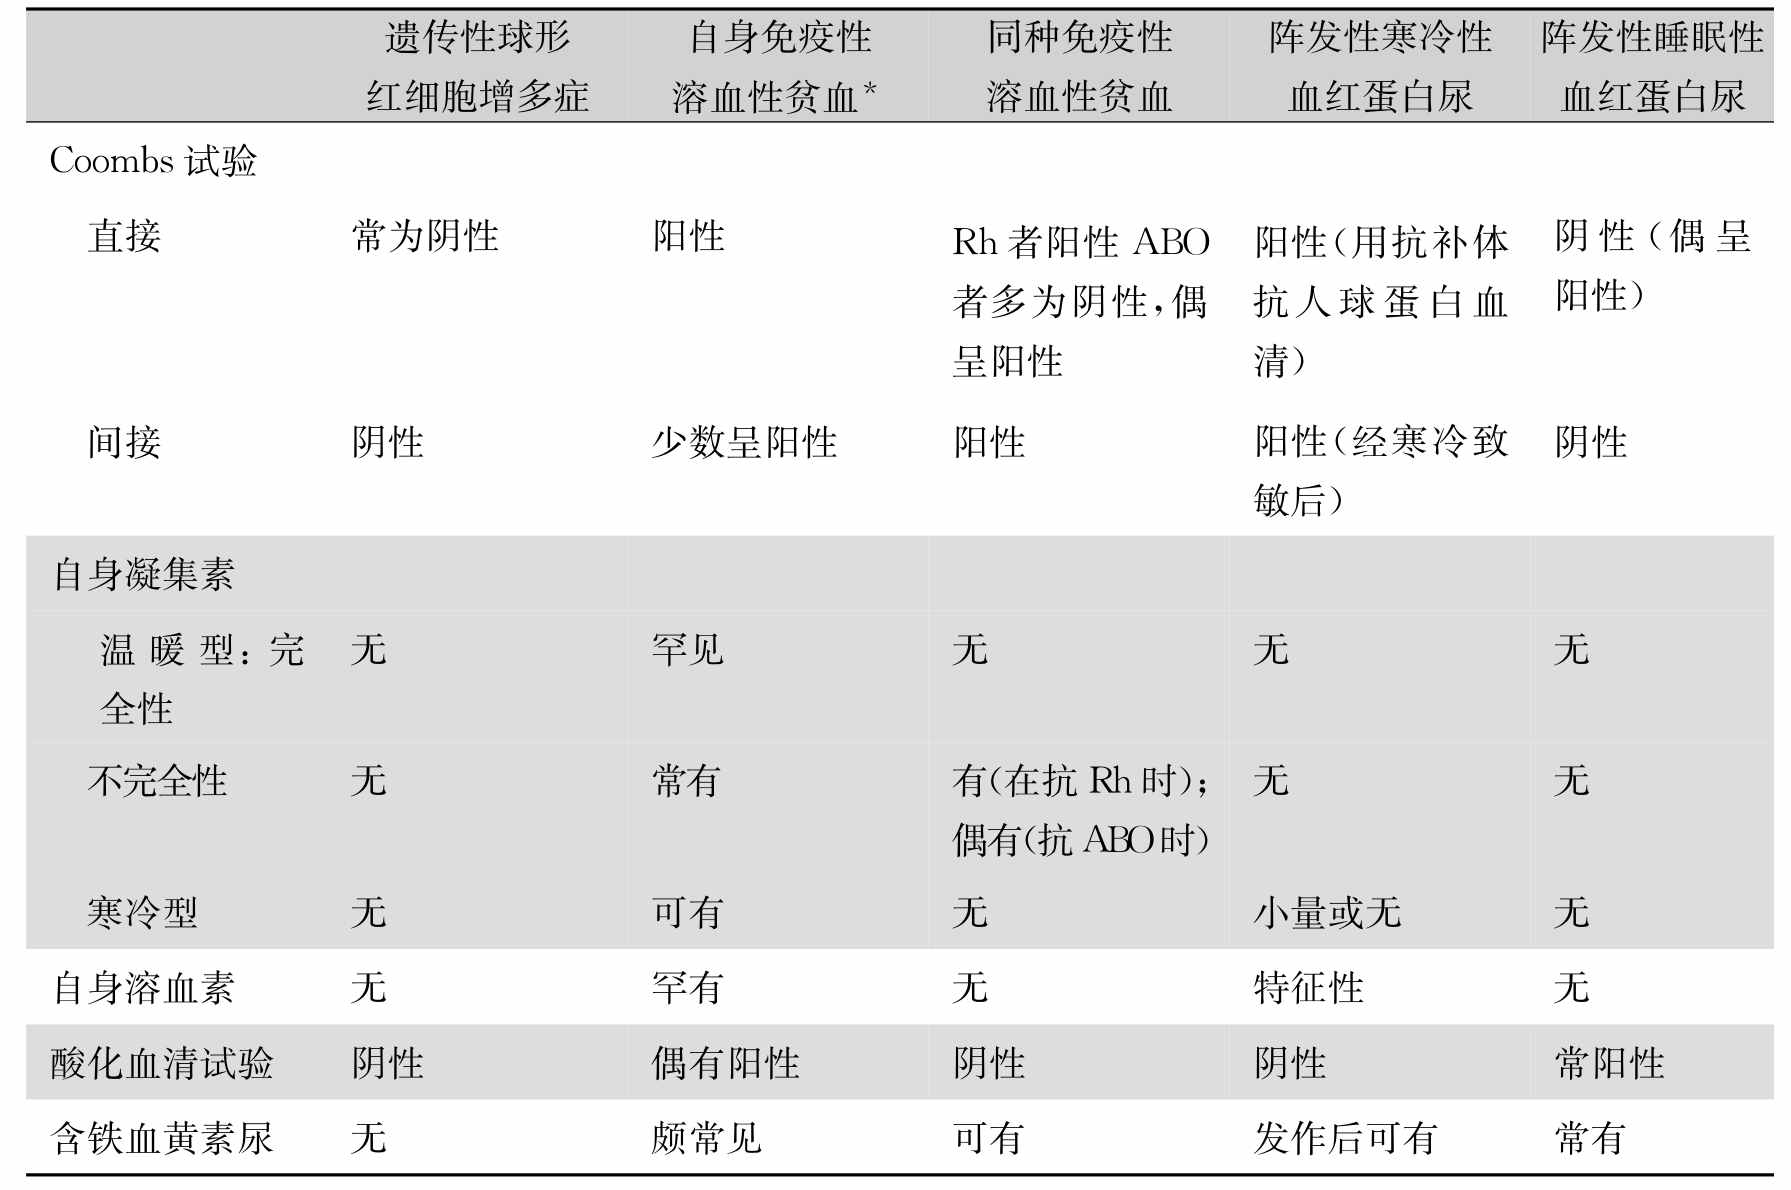
\includegraphics[width=\textwidth,height=\textheight,keepaspectratio]{./images/Image00182.jpg}
 \end{longtable}



\paragraph{五、红细胞碎片综合征}

红细胞碎片综合征(red cell fragment
syndrome)包括微血管病性溶血性贫血(microangiopathic hemolytic
anemia)和心源性溶血性贫血(cardiac hemolytic
anemia)。前者见于急性肾衰竭、恶性高血压、转移癌、血栓性血小板减少性紫癜、弥散性血管内凝血、妊娠中毒症、胎盘早期剥离、溶血性尿毒症综合征、阵发性行军性血红蛋白尿、暴发型紫癜、肝肾移植排斥、败血症及海绵状血管瘤等。后者见于心脏外科手术后或重症心瓣膜病患者。

微血管性溶血性贫血的机制为,上述各种疾病引起微血管广泛的纤维蛋白及血小板沉积、血栓形成,或其他因素导致微血管管腔变窄,红细胞在流经时受到过多的挤压、撕裂,而导致溶血。其实验室特点是:①血管内溶血:血浆游离血红蛋白含量增加,结合珠蛋白含量下降,出现血红蛋白尿或含铁血黄素尿。②周围血出现红细胞碎片,皱缩红细胞、刺细胞、三角形及钢盔形细胞等异形红细胞。③网织红细胞增多。④血小板减少。

心源性溶血性贫血的血涂片检查结果似微血管性溶血性贫血,但前者有心脏外科手术史或重症心瓣膜病病征,心脏瓣膜和大血管异常导致血流动力学改变,红细胞在循环中受涡流的拍打、冲击而受到机械性损伤,导致溶血。

\paragraph{六、动植物因素所致的溶血性贫血(参见第120节)}

\paragraph{七、物理因素所致的溶血性贫血(参见第120节)}

\protect\hypertarget{text00261.html}{}{}

\section{114 造血不良性贫血}

造血不良性贫血可分为血红蛋白合成障碍、核成熟障碍及骨髓衰竭所致贫血三大类。血红蛋白合成障碍所致的贫血,多为低色素性贫血,通常对铁剂(有些对维生素B\textsubscript{6}
等)治疗反应良好。核成熟障碍性贫血,为高色素大细胞性贫血,通常对维生素B\textsubscript{12}
或叶酸治疗反应良好。骨髓衰竭所致贫血为正细胞性贫血,一般抗贫血治疗效果不佳;仅部分病例在除去原发病因或脾摘除后贫血得到缓解。对于造血不良性贫血的诊断与鉴别诊断,病史的询问和体格检查应力求详细,特别要注意饮食、营养、职业、药物或放射能接触、月经、生育、哺乳及全身性慢性病等病史。体检须注意外胚叶组织,神经系统,肝、脾、淋巴结及骨骼系统等的异常体征。

\subsection{114.1 血红蛋白合成障碍}

原卟啉与铁原子组成血红素,后者与珠蛋白肽链结合形成血红蛋白分子。其中任何一种物质缺乏或发生代谢紊乱,均会引起血红蛋白合成障碍导致贫血。这类贫血包括缺铁性贫血和其他非缺铁所致低色素性贫血。

\subsubsection{114.1.1 缺铁性贫血}

缺铁性贫血是由于体内储存铁缺乏,不能满足正常红细胞生成的需要时所发生的贫血。临床上见到的血红蛋白合成障碍所致贫血,大多是由于铁缺乏。铁是人体必需的微量元素,存在于人体所有的细胞内,其不仅是合成血红蛋白所必需,还参与体内的多种生物化学过程,多种酶发挥活性也需要铁的存在。因此,缺铁除导致贫血外,还可导致黏膜组织变化和外胚叶组织营养障碍等其他细胞功能紊乱。

膳食中缺铁或慢性失血病史,体检发现外胚叶改变尤其是反甲,以及实验室检查证明为小细胞低色素性贫血,强烈提示缺铁性贫血诊断的可能性。

缺铁性贫血的血象呈小细胞低色素性贫血。血色指数常下降至0.5。小红细胞增多,并有红细胞大小不等与异形红细胞。红细胞变薄,中心缺色。往往出现较多的多色性与嗜碱性点彩红细胞。红细胞直径曲线(Price-Jones曲线)高峰左移(图\ref{fig33-6}),基底增宽。网织红细胞不增多或轻度增多。重症病例白细胞数和血小板数也减少。

\begin{figure}[!htbp]
 \centering
 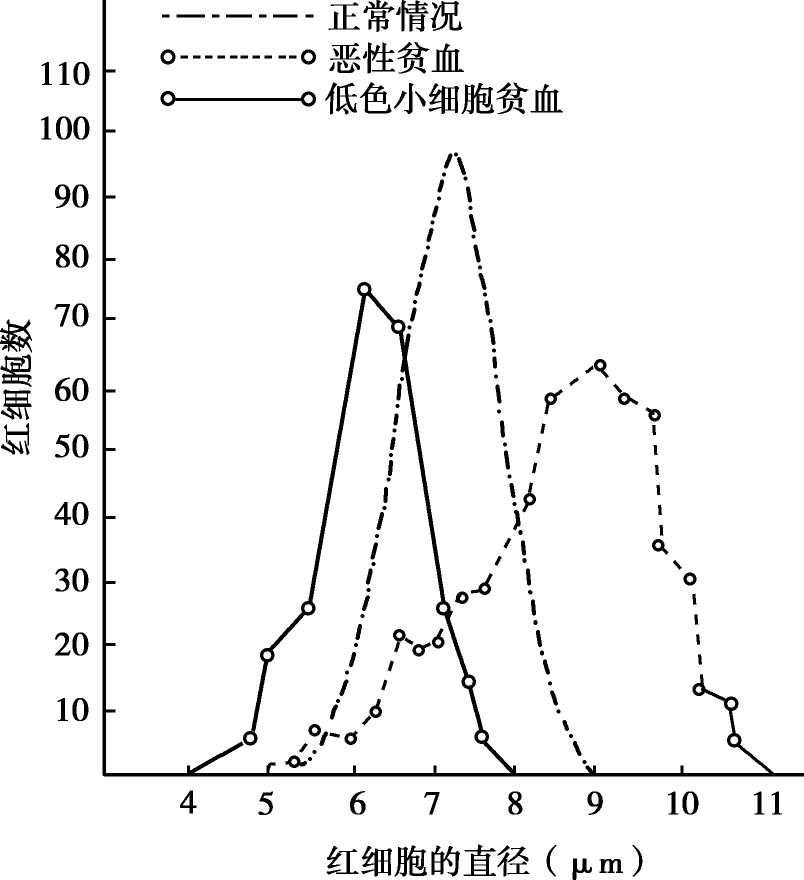
\includegraphics[width=2.76042in,height=3.01042in]{./images/Image00183.jpg}
 \captionsetup{justification=centering}
 \caption{红细胞直径曲线图}
 \label{fig33-6}
  \end{figure} 

铁缺乏如同时伴有胱氨酸缺乏时,临床表现为外胚叶组织病变:头发蓬松,皮肤萎缩、干燥、羊皮纸样,指、趾甲脆薄而扁平或凹陷(反甲)、易分裂成层等。铁缺乏伴有B族维生素缺乏时,可有舌炎、口角炎、食管黏膜萎缩。部分患者有吞咽困难,须与食管癌区别。如吞咽困难伴有低色素性贫血及胃盐酸缺乏,称为普-文综合征。

缺铁性贫血的诊断标准是:①小细胞低色素性贫血:男性Hb<120g/L,女性Hb<110g/L,孕妇Hb<100g/L;MCV<80fl,MCH<26pg,MCHC<310g/L;红细胞有明显低色素表现。②有明确的缺铁性病因和临床表现。③血清铁<10.7μmol/L,总铁结合力>64.4μmol/L。④血清铁饱和度<15\%。⑤骨髓铁染色显示骨髓小粒可染铁消失,铁粒幼细胞<15\%。⑥红细胞游离原卟啉>0.9μmol/L。⑦血清铁蛋白<14μg/L。⑧铁剂治疗有效。符合第1条和第2~8条中任何两项以上者可确诊(图\ref{fig33-7})。

\begin{figure}[!htbp]
 \centering
 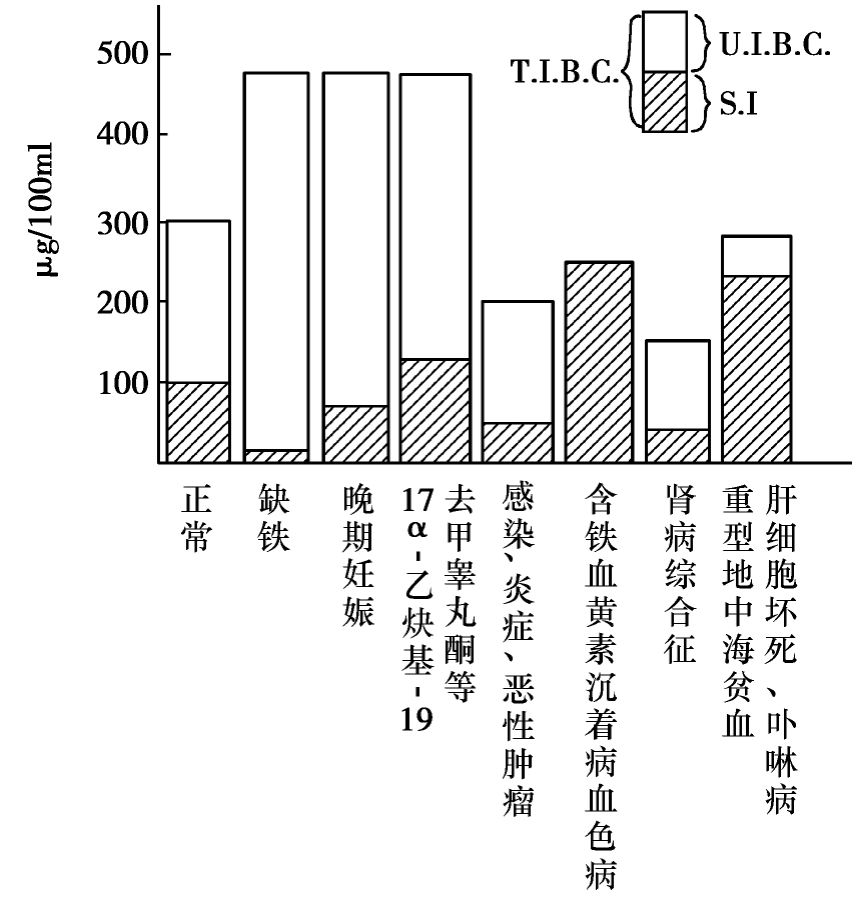
\includegraphics[width=2.875in,height=3in]{./images/Image00184.jpg}
 \captionsetup{justification=centering}
 \caption{各种疾病的血清铁和铁结合力}
 \label{fig33-7}
  \end{figure} 

T.I.B.C总铁结合力; U.I.B.C不饱和铁结合力; S.I血清铁

本病需与其他非缺铁所致低色素性贫血相区别。这类贫血发病率较低,包括:珠蛋白生成障碍性贫血、铁粒幼细胞性贫血、慢性疾病性贫血、慢性铅中毒及载铁蛋白缺乏性贫血等。这类贫血根据以下的共同特点有别于缺铁性贫血:①体内贮备铁含量增加,包括骨髓含铁血黄素含量增加、骨髓铁粒幼细胞或含铁红细胞(siderocytes)增多;②总铁结合力多减低。

与几种常见的非缺铁低色素性贫血的具体鉴别如下:地中海贫血时,患者常有家族史,血片中可见多量靶形红细胞,血红蛋白电泳测定血红蛋白F与A2含量增多,患者血清铁、转铁蛋白饱和度及骨髓可染铁均增多。铁粒幼细胞性贫血,主要原因为铁利用障碍,血清铁增高而总铁结合力正常,骨髓中铁颗粒明显增多,可见多数环状铁粒幼细胞,粗而多的铁质颗粒常排列成衣领状,围绕着有核红细胞的胞核。慢性疾病性贫血,其机制较为复杂,有慢性原发病的存在,实验室检查特点为血清铁蛋白增高,骨髓中铁粒幼细胞减少,巨噬细胞内铁及含铁血黄素颗粒明显增多。慢性铅中毒的特点为点彩红细胞增多,尿中粪卟啉半定量阳性。

缺铁性贫血是许多疾病的共同表现,在明确贫血性质为缺铁后,还必须查明导致缺铁的病因。缺铁性贫血病因甚多,一般分为四类:①慢性失血;②铁需要量增多;③铁吸收障碍;④食物中铁缺乏。致病原因可为单项或几项联合致病,有人统计47例缺铁性贫血,单项原因者21例,两项原因或两项以上者占26例(表\ref{tab33-10})。

\begin{longtable}{c}
 \caption{47例缺铁性贫血发病原因的分析}
 \label{tab33-10}
 \endfirsthead
 \caption[]{47例缺铁性贫血发病原因的分析}
 \endhead
 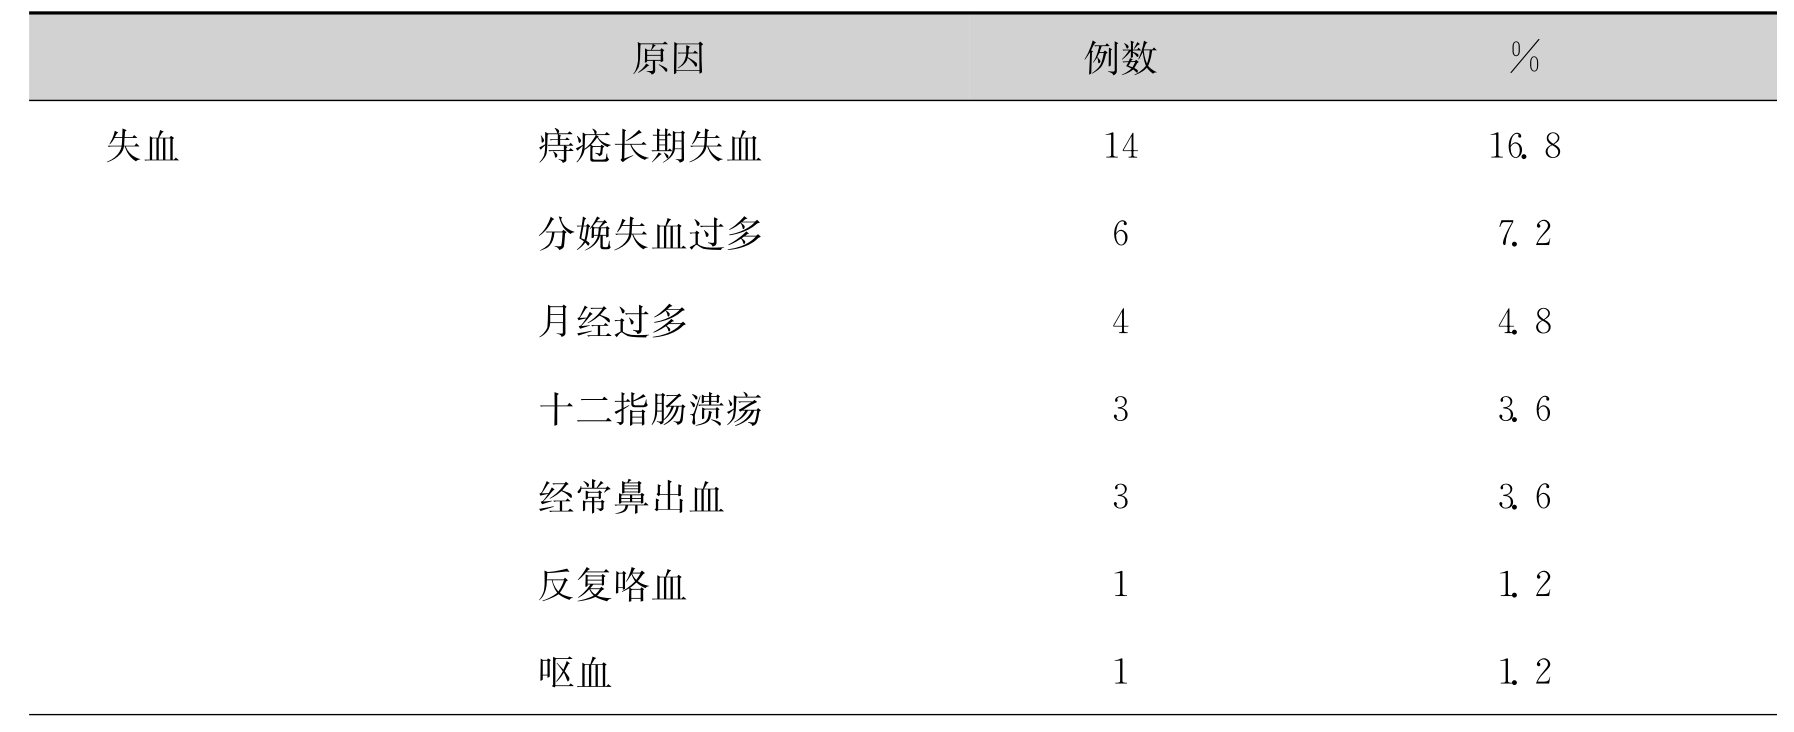
\includegraphics[width=\textwidth,height=\textheight,keepaspectratio]{./images/Image00185.jpg}\\
 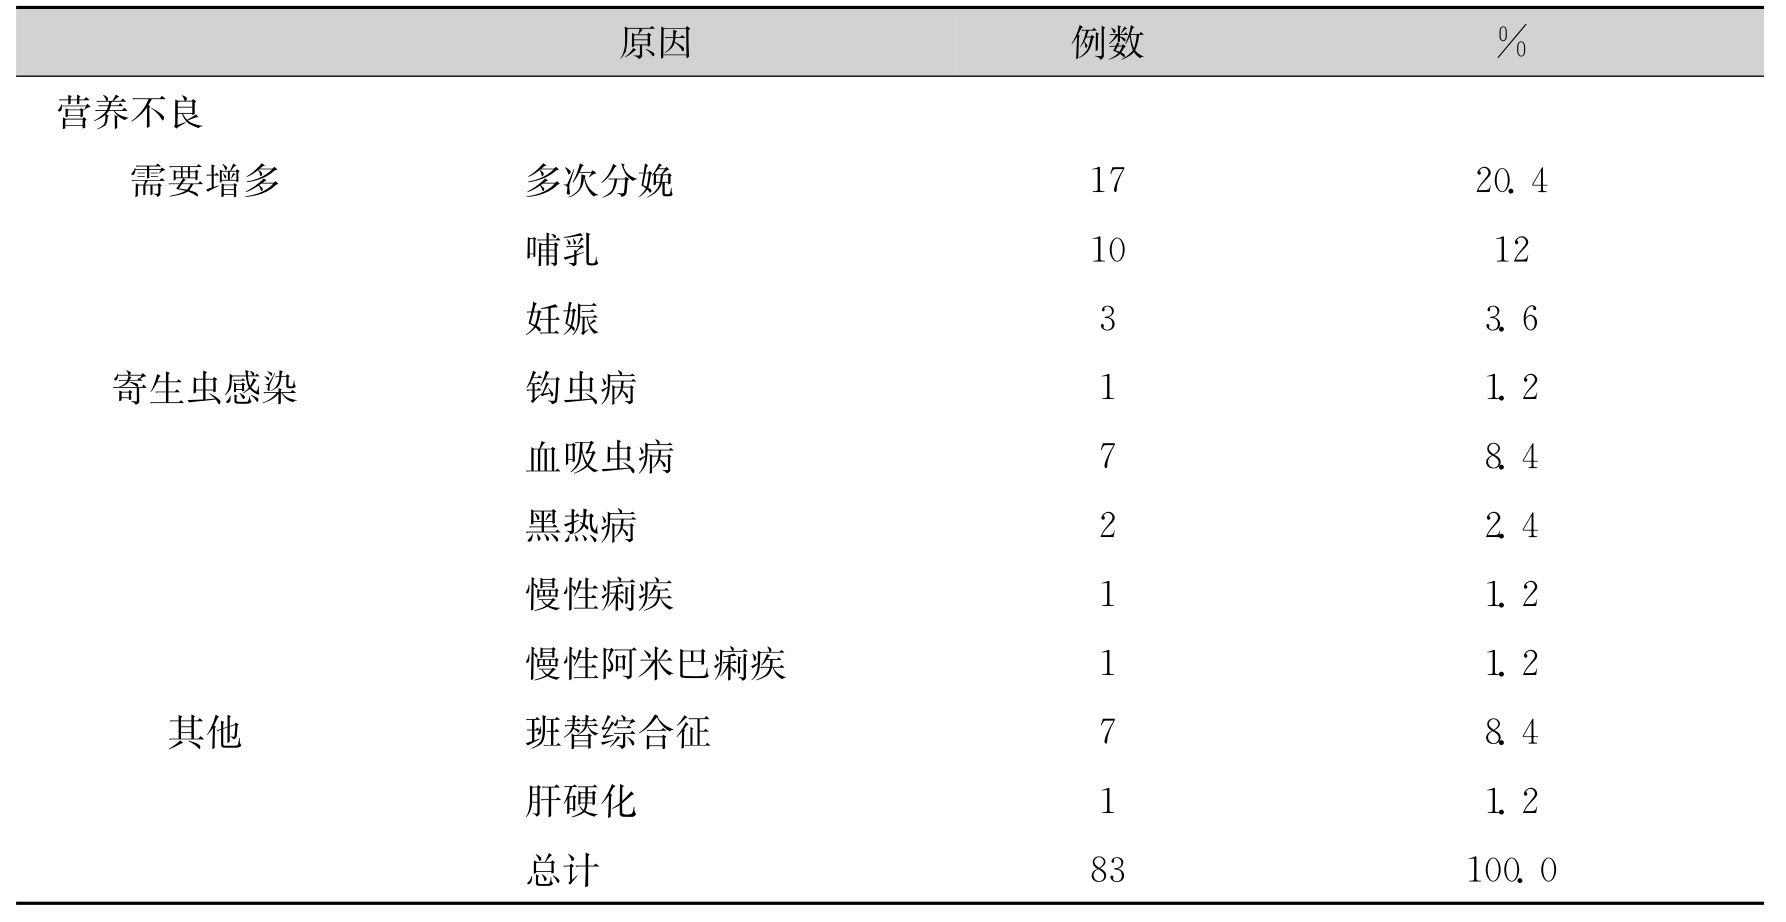
\includegraphics[width=\textwidth,height=\textheight,keepaspectratio]{./images/Image00186.jpg}
 \end{longtable}

\paragraph{一、慢性失血性贫血}

慢性失血是缺铁性贫血最常见的病因之一,长期小量出血比一次大量出血更易发生缺铁性贫血。失血后贫血是各类贫血中最常见的原因,且占各种病因的大多数。缺铁原因乃由于失血。出血来源最常为胃肠道疾病如痔疮、胃十二指肠溃疡、息肉及钩虫病等,缺铁性贫血常是胃肠道肿瘤的首发表现。其次为月经过多,此外多次献血、多次妊娠、咯血、PNH也是慢性失血的常见原因。

\paragraph{二、铁需量增加性贫血}

本病由于多种缺铁原因致病,主要是由于妊娠、分娩、哺乳和月经等生理铁需要量明显增加,而食物中铁含量和肠道吸收铁的功能,均不能补偿这种需要增加所致。

\subparagraph{(一)原发性低色素性贫血}

本病又称晚期萎黄病(late
chlorosis),其特点是:①患者几乎全部为中年女性(30~45岁);②外胚叶组织病变及普-文综合征特别明显;③胃液从低酸至无酸,但盐酸并非必然缺乏,对组胺也非全无反应,完全的胃酸缺乏罕见。

\subparagraph{(二)早期萎黄病}

本病近年甚少发现。发病年龄在少女青春期,而胃酸分泌正常,可与晚期萎黄病相区别。

本病是以面色苍白带绿色及血清铁明显降低为特征。主要症状是全身衰弱、乏力、嗜睡以及其他贫血症状。患者颜面苍白并带绿色与轻度水肿,月经减少。有静脉血栓形成倾向,胃酸分泌并无障碍。致病因素比较复杂,一般认为少女青春期生理性铁需要量增加为主要原因。

\subparagraph{(三)妊娠期缺铁性贫血}

根据中山医学院检查1332名孕妇血象,发现362名合并贫血,占27.2\%。年龄大,胎数多较易罹患。此组贫血以正常红细胞性贫血最多,小细胞低色素性贫血次之,而巨幼细胞性贫血只占2例。临床上所见绝大多数缺铁性贫血为小细胞低色素性贫血,但根据笔者医院材料,孕妇合并缺铁,常呈正常红细胞性贫血,只有轻度低色素现象。这可能与贫血程度较轻及罹病时间较短有关。

在临床上,孕妇有苍白和水肿,血红蛋白在100g/L以下,骨髓无巨幼红细胞,可诊断为妊娠期缺铁性贫血。本病需与妊娠期间血容量增加所致的“生理性贫血”(“假性贫血”)相区别。后者血红蛋白量仅波动在正常低值附近,较少下降至100g/L以下,且红细胞并无缺铁特征,可与本病相区别。

\paragraph{三、铁吸收障碍性贫血}

食物中所含的铁,大都为三价铁,需转化为二价铁方能被上段小肠所吸收。对铁吸收有重要关系的因素是:①胃盐酸;②十二指肠液;③维生素C;④小肠蠕动速度;⑤身体对铁的需要(缺铁的机体较已被铁饱和的机体吸收铁更多)。

由于铁吸收障碍所致缺铁性贫血,可见于胃大部分切除后、胃癌、膈疝、慢性痢疾、吸收不良综合征等。

\paragraph{四、食饵性缺铁性贫血}

肉类与青菜中含有足量的铁,一般可得到足够的铁供应。解放后我国人民生活水平大大提高,现在国内仅偶见于少数习惯偏食的人,罹患此型贫血。

\subsubsection{114.1.2 铁粒幼细胞性贫血}

铁粒幼细胞性贫血(sideroblastic
anemia)是由于多种不同原因引起的铁利用障碍性贫血。其发病机制主要与血红素的合成障碍有关。血红素的生物合成过程是先由甘氨酸和琥珀酰辅酶A等合成氨基酮戊酸,再转化为卟胆原、尿卟啉、粪卟啉和原卟啉,最后在血红素合成酶的作用下与二价铁结合成血红素。一旦上述合成过程中某些酶有缺陷,均会影响血红素的合成。此时红细胞对铁的摄入增加,而铁不能得到很好利用,堆积在线粒体中,形成环状铁粒幼细胞。

此型贫血分为遗传性铁粒幼细胞性贫血和获得性铁粒幼细胞性贫血两大类。后者又分为特发性与继发性。

遗传性铁粒幼细胞性贫血发病率甚低,为伴性隐性遗传性疾病,见于男性,出生后还可存活多年,肝活检可证明有大量含铁血黄素沉着,并可发展为含铁血黄素沉着症,未见有临终期转变为白血病的报道。

原发性获得性铁粒幼细胞性贫血发病年龄较晚,多在60岁以上发病,呈慢性经过,少数病例临终期转变为急性粒细胞型或单核细胞型白血病。目前认为本病是造血干细胞克隆性疾病,与遗传无关。骨髓中除有较多的环形铁粒幼细胞外,常伴有红系、粒系和(或)巨核系的病态造血。目前已将此病归为骨髓增生异常综合征的一种,称难治性铁粒幼细胞性贫血。临床贫血程度轻重不一,常伴有白细胞和(或)血小板减少。

继发性的原因有铅中毒、抗结核药物作用、酒精中毒、支气管癌、类风湿关节炎、地中海贫血等。继发于铅中毒者可由于铅抑制血红素的合成所致;继发于抗结核药物,如异烟肼等可能是维生素B6的拮抗物。药物或毒物引起的铁粒幼细胞性贫血,只要停止服用或接触有关的药物或毒物,贫血即可逐渐消失。

患者有低色素性贫血而对铁剂治疗无效,且骨髓中证实大量铁粒幼细胞存在时,需考虑本病的诊断。实验室检查特点为:①呈正常细胞低色素性或小细胞低色素性贫血;②网织红细胞正常或轻度增多;③骨髓幼红细胞明显增生,铁染色示含铁血黄素显著增多,铁粒幼红细胞增多,可见环形铁粒幼细胞>15\%,后者主要累及较晚期幼红细胞,粗大的铁颗粒排列于胞核周围,形成完全的或不完全的环形;④血清铁、铁蛋白增高,血清总铁结合力减低。

\subsubsection{114.1.3 载铁蛋白缺乏性贫血}

载铁蛋白缺乏性贫血(atransferrinemia)罕见。在先天性者,贫血较为严重,常有含铁血黄素沉着症。在获得性者,可见于肾病综合征、渗出性肠疾病、低蛋白血症、感染等疾病。这些疾病有载铁蛋白的丧失、合成障碍、分解增加及转移入炎症组织中,因此可引起载铁蛋白缺乏。载铁蛋白的缺乏使铁转运功能降低,血红蛋白合成障碍。临床特点是出现小细胞低色素性贫血,血清铁和总铁结合力非常低,血清蛋白电泳显示载铁蛋白含量明显下降,骨髓铁含量降低,铁剂治疗无效。

\subsection{114.2 核成熟障碍}

此类贫血少见,仅约占全部贫血病例的5\%以下。原因是缺乏维生素B\textsubscript{12}
或(及)叶酸;有些病例虽然不缺乏这类物质,但机体丧失了吸收或利用这类物质的功能。这两种物质的缺乏或代谢紊乱,主要引起骨髓幼稚红细胞核的成熟障碍。缺乏维生素B\textsubscript{12}
与叶酸时,脱氧核糖核酸(DNA)形成障碍,细胞核分裂周期中的DNA合成期(S期)延长,核成熟发生障碍,而胞浆中血红蛋白的合成正常。导致胞核与胞浆的发育不同步,细胞体积增大,呈现形态与功能均不正常的巨幼改变。这种改变可涉及红细胞、粒细胞及巨核细胞,且细胞未发育成熟即在骨髓内破坏,为无效生成。除造血细胞外,在更新较快的细胞,如胃肠道上皮细胞中也存在类似的改变,故本病常伴胃肠道症状。维生素B\textsubscript{12}
缺乏者,神经系统的细胞和髓质也常发生改变,出现神经系统症状。

此类贫血的临床特点是:①缓慢进行的大细胞性贫血,外周血红细胞平均体积增大,平均血红蛋白量增高,平均血红蛋白浓度正常,红细胞体积分布宽度曲线右移并扩大。白细胞和血小板也可减少;中性粒细胞常出现核分叶过多现象。②骨髓的有核细胞明显增多并有巨幼变。幼红细胞可占30\%~60\%,其中多为巨型幼红细胞,该类细胞的特点是体积较大,胞核的发育较胞质迟缓,核染色质排列成细网状。粒系和巨核系亦有类似改变。③常有口腔、胃肠道及神经系统的损害。④维生素B\textsubscript{12}
与叶酸治疗对大多数病例奏效。此类贫血应与正常幼红细胞性大细胞性贫血(normoblastic
macrocytic
anemia)相区别,后者仅周围血出现大细胞而骨髓幼红细胞形态正常,且其原因并非缺乏维生素B\textsubscript{12}
与叶酸,而是继发于其他疾病如某些类型溶血性贫血。

从治疗观点出发,对巨幼细胞性贫血要进一步区分为维生素B\textsubscript{12}
或叶酸缺乏,或两者同时缺乏。临床表现和原发病在鉴别诊断上最为重要。叶酸缺乏的消化道症状较明显,维生素B\textsubscript{12}
缺乏则神经系统症状较明显;胃游离盐酸缺乏多见于维生素B\textsubscript{12}
缺乏;继发于营养不良、吸收不良综合征、妊娠、肝硬化、慢性溶血性贫血及抗癫痫药物治疗所致的巨幼细胞性贫血,有利于叶酸缺乏的诊断;分别用维生素B\textsubscript{12}
或叶酸作诊断性治疗是一个有鉴别意义的方法;有条件的实验室还可测定血清维生素B\textsubscript{12}
与血清叶酸的含量,提供确实的诊断根据。

核成熟障碍所致贫血主要分为下列三组:

\subsubsection{114.2.1 恶性贫血}

恶性贫血国内少见,本病的基本缺陷在于胃内因子分泌障碍。胃内因子产生于胃体和胃底,这是一种胃黏蛋白,有加速维生素B\textsubscript{12}
在小肠黏膜吸收的作用。因此本病患者存在维生素B\textsubscript{12}
吸收障碍,产生维生素B\textsubscript{12}
的相关临床表现。胃内因子缺乏的发病机制尚待阐明,可能与遗传或自身免疫因素有关。

典型病例有下列三组病征:①巨幼细胞性贫血;②舌炎与胃酸缺乏;③周围神经变性与脊髓联合变性。神经系统症状主要有:周围神经变性引起肢体麻木感或感觉异常;脊髓后索变性引起腱反射消失,肌张力减弱,位置觉紊乱;反射亢进与肌张力增强等。神经系统症状可为本病的突出表现,甚至患者被疑为周围神经炎或多发性硬化而首先就诊于神经科。

血象出现巨红细胞,骨髓显示巨幼红细胞增生。胃酸缺乏,空腹血清促胃液素显著增高。有条件可检测内因子及其抗体。

本病的诊断一般可根据临床特征、血象与骨髓象、胃液分析、维生素B\textsubscript{12}
的疗效以及长期随诊而确定。血清维生素B\textsubscript{12}
测定、放射性核素维生素B\textsubscript{12}
吸收试验(表\ref{tab33-11}),也有助于诊断。

表\ref{tab33-11} 维生素B\textsubscript{12}
和叶酸缺乏时的放射性核素维生素B\textsubscript{12} 吸收试验

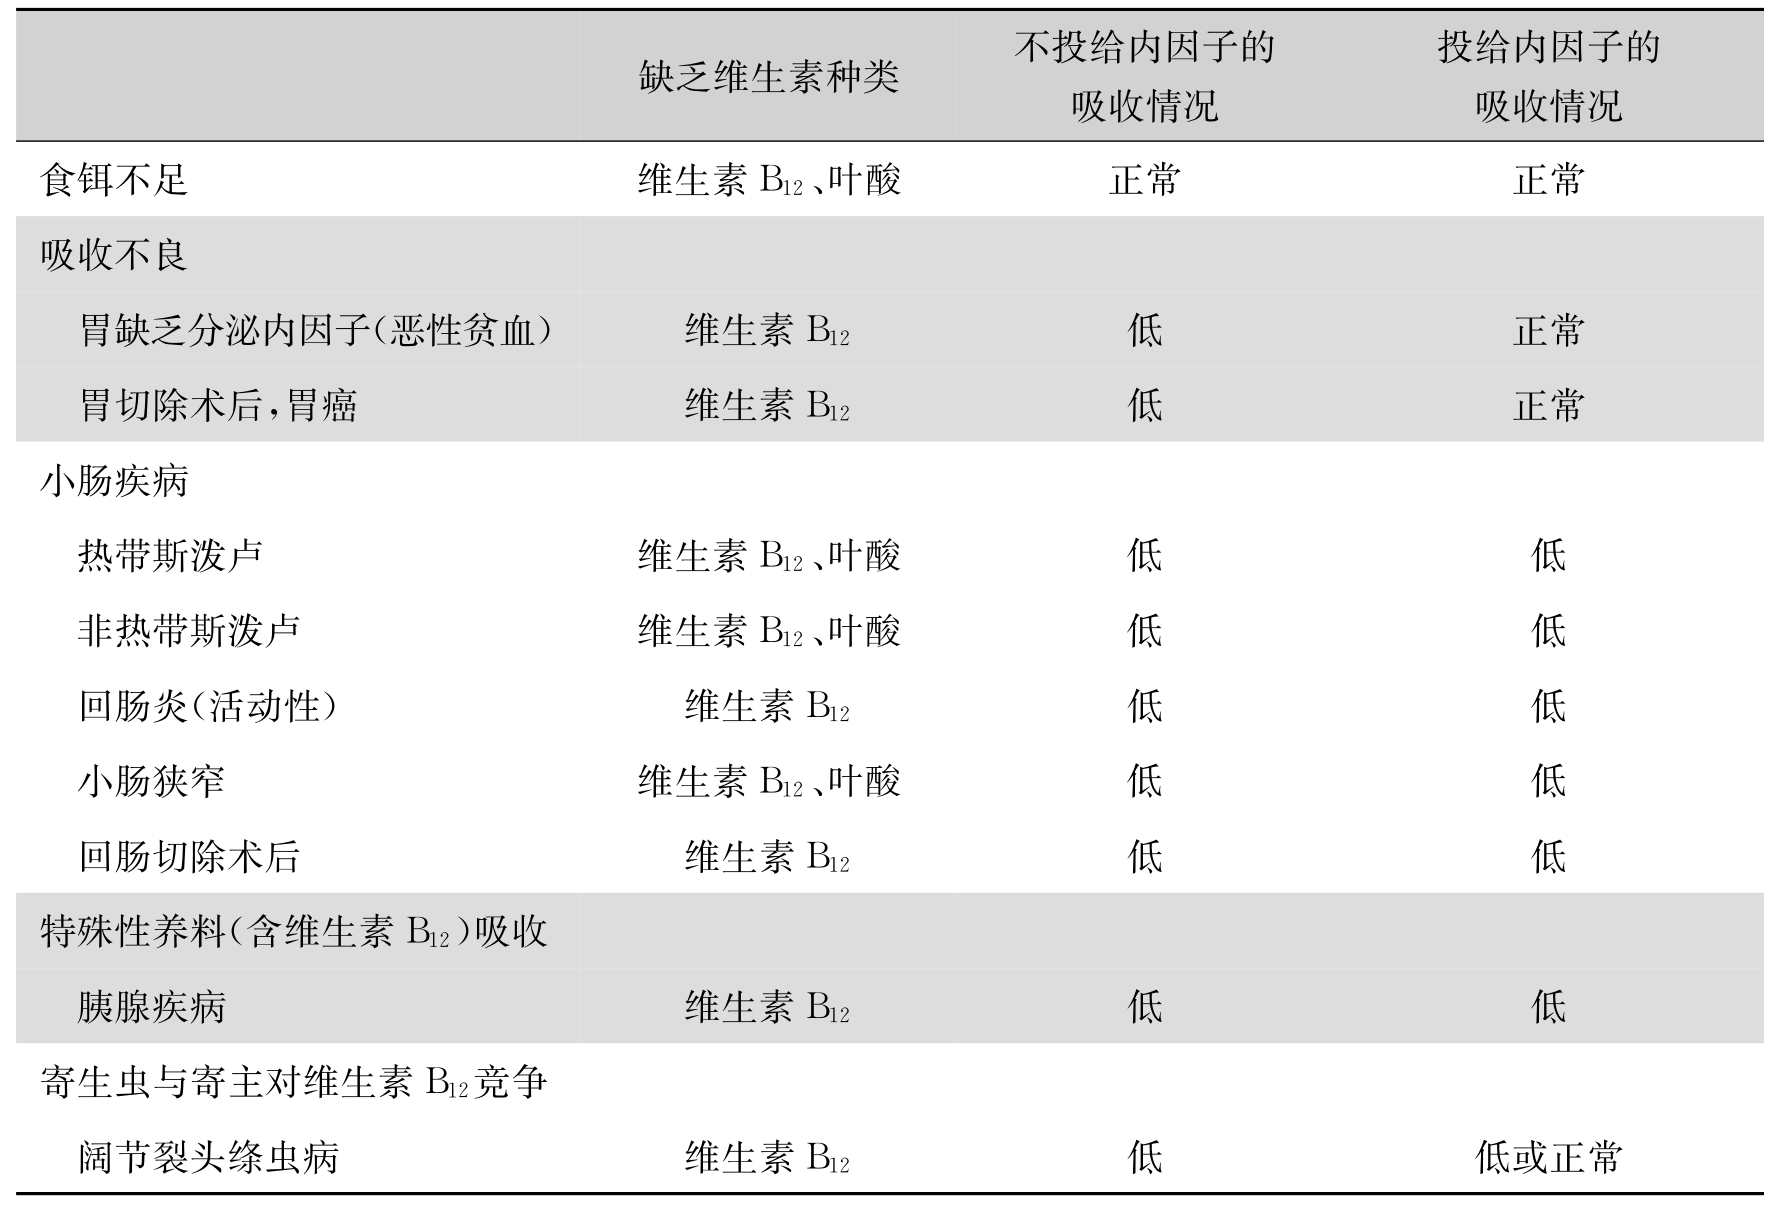
\includegraphics[width=5.92708in,height=4.03125in]{./images/Image00187.jpg}

本病首先应与红白血病相区别,后者用维生素B\textsubscript{12}
治疗无效,且幼稚红细胞形态有明显的病理改变。在再发期病例常有溶血现象,应注意与其他类型溶血性贫血相区别。患者有食欲减退、胃游离盐酸缺乏,尚需与胃癌相区别;但须注意,本病可为胃癌的前期。

\subsubsection{114.2.2 非恶性贫血所致核成熟障碍贫血}

\paragraph{一、营养性巨幼细胞性贫血}

营养性巨幼细胞性贫血的原因大多是膳食质量不佳,缺乏新鲜蔬菜或肉、蛋类食物,或烹调时间过长,叶酸遭到破坏。并且常伴有叶酸的需要增加,导致叶酸缺乏。维生素B\textsubscript{12}
缺乏相对少见,因为维生素B\textsubscript{12}
的吸收存在肠肝循环,完全素食者(不吃任何动物来源的食物)也需10~15年才出现维生素B\textsubscript{12}
缺乏的表现。临床症状以消化系统症状和贫血症状较为突出。可并发贫血性心脏病。常有舌乳头萎缩及维生素缺乏症的其他表现,但无深感觉异常与神经病理反射。

本病的诊断主要根据:①有维生素B\textsubscript{12}
及(或)叶酸生理需要量增加或偏食而致营养不良的病史;②巨幼细胞性贫血的血液学改变;③叶酸及维生素B\textsubscript{12}
浓度测定;若无条件进行该项检查,可予叶酸和维生素B\textsubscript{12}
进行治疗性实验,疗效显著亦支持诊断;④除外其他原因所致的巨幼细胞性贫血。

本病根据下列几点可与恶性贫血相区别:①胃游离盐酸大多存在;②无脊髓联合变性的神经系改变;③维生素B\textsubscript{12}
、叶酸治疗都有效,治愈后不给药也不复发;④常合并缺铁性贫血,形成所谓“二形性”贫血------低色素性巨幼红细胞性贫血。

\paragraph{二、斯泼卢(Sprue)}

本病常以慢性腹泻(脂肪泻)为临床特征,可引起巨幼细胞性贫血。本病与恶性贫血的区别,主要根据:①本病时胃液分析有游离盐酸存在;②脂肪泻;③X线钡餐检查小肠有特征性改变,而恶性贫血则无此改变;④无脊髓联合变性的表现。

\paragraph{三、肝病性巨幼红细胞性贫血}

肝病可合并贫血,也可不合并贫血。国外有人统计一组肝病患者132例,其中不合并贫血者占22.7\%,大细胞性贫血占32.6\%,正细胞性贫血占30.3\%,小细胞贫血占14.4\%。肝病呈巨幼细胞性贫血者有慢性弥漫性肝实质病变的证据,较常见者为肝硬化。其原因可能由于肝病时食欲不振而致食入叶酸(主要)与维生素B\textsubscript{12}
(次要)不足所致。

\paragraph{四、并发于胃癌或胃切除术后巨幼细胞性贫血}

胃癌与胃切除术后可有胃内因子分泌不足,影响维生素B\textsubscript{12}
(所谓外因子)的吸收而致病。

\paragraph{五、慢性肠病所致巨幼细胞性贫血}

肠狭窄、肠瘘管、肠切除术或吻合术后、糙皮病、慢性痢疾或慢性胰腺炎等,可由于维生素B\textsubscript{12}
与叶酸吸收不足,或微生物与宿主对维生素B\textsubscript{12}
的竞争作用而引起巨幼细胞性贫血。

\paragraph{六、阔节裂头绦虫病}

本病的血象和骨髓象可与恶性贫血相似,唯一病情较急,胃酸多存在。维生素B\textsubscript{12}
的缺乏由于阔节裂头绦虫在肠内与宿主竞争维生素B\textsubscript{12}
所致。本绦虫在国内曾发现于东北地区。

\paragraph{七、药物所致巨幼红细胞性贫血}

乙胺嘧啶、苯妥英钠等可干扰人体内叶酸代谢,引起巨幼细胞性贫血。

\subsubsection{114.2.3 其他类型巨幼细胞性贫血}

少数巨幼细胞性贫血并非由于缺乏维生素B\textsubscript{12}
或叶酸所致。有人将白血病、恶性肿瘤、某些感染性疾病及慢性肾衰竭所致的巨幼细胞性贫血,归类入“难治性”巨幼细胞性贫血范畴。这些疾病骨髓涂片呈巨幼细胞性贫血骨髓象,伴有或不伴有周围血大细胞性贫血改变。诊断时须首先除外维生素B\textsubscript{12}
或叶酸缺乏所致的巨幼细胞性贫血。

\subsection{114.3 骨髓衰竭}

骨髓衰竭所致贫血包括:慢性疾病性贫血、中毒性贫血、脾大的脾功能亢进性贫血(内分泌障碍性贫血、骨髓痨性贫血、再生障碍性贫血等。骨髓衰竭可分为真性衰竭(true
failure)与相对性衰竭(relative
failure)。前者骨髓造血功能减低,不足以代偿红细胞生理性的损耗(如再生障碍性贫血等);后者骨髓造血功能虽有一定程度的增加,但远不如正常的骨髓功能足以代偿红细胞病理性的加速损耗(如骨髓痨性贫血等)。

临床表现和实验室检查如能排除失血后贫血、溶血性贫血,以及造血不良性贫血中的血红蛋白合成障碍所致贫血与核成熟障碍所致贫血,并有损害骨髓造血功能的病因存在时,符合骨髓衰竭所致贫血的诊断。

\subsubsection{114.3.1 慢性疾病导致的贫血}

慢性疾病性贫血本身并非一个独立的疾病,而是感染或某些慢性全身性疾病的一种表现。慢性病贫血的发病率甚高,仅次于缺铁性贫血,是住院患者中最多见的贫血。慢性病贫血一般都伴有基础疾病,持续时间多在1~2个月以上。这种情况可见于慢性感染(如肺结核、肺脓肿)、结缔组织病(系统性红斑狼疮、类风湿关节炎)、恶性肿瘤(乳腺癌、恶性淋巴瘤)及某些系统性慢性疾病(如肾病、肝病及内分泌疾患)等。在临床上,本型贫血较为常见,尤其常见于内科住院患者。因此,对未明原因的贫血,须注意有无各种慢性感染或全身性疾病;而这些慢性感染和全身性疾病的确诊又能提供此种贫血的诊断根据。从全面的与细致的临床检查与各项辅助检查,所获得的原发病的证据,是诊断慢性疾病性贫血的首要步骤。这些贫血的特点是贫血长期保持稳定,且程度较轻而无需治疗,但有少数也可较为严重,如见于肾衰竭或恶性肿瘤时。

本类贫血的发生机制复杂,目前认为主要与红细胞寿命缩短、EPO分泌不足或骨髓对EPO反应下降、铁的释放及利用障碍等因素有关。实验室检查特点:①贫血通常为正细胞性正色素性,偶呈小细胞性低色素性,白细胞总数和血小板数一般在正常范围。②血清铁、血清总铁结合力(图\ref{fig33-7})、载铁蛋白饱和度(tansferrin
saturation)及骨髓铁粒幼细胞数均下降,血清铁蛋白及单核-吞噬细胞系统铁含量正常或增多。以放射性铁标志的无生存能力的红细胞输给患者,仅有不到40\%(正常人55\%~70\%)的铁被用于血红蛋白的合成。证明铁自单核-吞噬细胞系统流入血浆受到障碍,即所谓网状内皮铁阻滞(RE
iron
block),是本型贫血的特点之一。因此有人又称本型贫血为缺铁性贫血合并网状内皮组织铁质沉着症。③用放射性核素测定可见患者的红细胞寿命缩短,但血清胆红素正常。本型贫血和通常的缺铁性贫血,骨髓铁粒幼细胞数目均减少,但前者的骨髓涂片细胞外铁含量仍保持正常或增多,而缺铁性贫血则减少。本型贫血对一般抗贫血治疗效果欠佳,尚需与单纯红细胞再生障碍贫血相区别,根据原发病的存在可资区别。

下面根据具体的原发疾病分类讲述:

\paragraph{一、感染性贫血}

急、慢性感染均可引起贫血,常见感染病原体有细菌、病毒、寄生虫等。感染的疾病有呼吸道炎症、慢性肠炎、妇科炎症、细菌性心内膜炎、伤寒、结核等。感染性贫血的发病机制是:①骨髓对贫血的代偿功能失常:动物实验证明,缺氧和给予红细胞生成素只能引起部分反应,而不能引致红细胞增多症,可能由于骨髓对红细胞生成素反应性降低所致;②单核-吞噬细胞系统受感染刺激,对红细胞的破坏增加,红细胞寿命缩短;③网状内皮铁阻滞,幼红细胞铁利用不良;④慢性胃肠道炎症、营养不良致铁吸收减少,合并慢性出血时铁丢失过多。

实验室检查特点:①慢性感染所致贫血,程度多为轻到中度,一般表现为正色素、正细胞性,有些可为小细胞低色素性贫血。②血清铁和载铁蛋白饱和度降低。③骨髓涂片有核红细胞及粒/红比值大致正常,无明显红系增生表现。铁粒幼细胞减少,单核-巨噬细胞内铁储存量增加。本病的诊断主要是找到引起贫血的原发感染性疾病,并除外其他原因引起的贫血。

\paragraph{二、恶性肿瘤所致贫血}

恶性肿瘤所致贫血是指造血组织以外的各种肿瘤引起的贫血。其贫血表现类型和程度因恶性肿瘤种类、病程、治疗方法不同而差别较大。恶性肿瘤所致贫血的形成机制复杂多样,主要与以下因素有关:①造血祖细胞功能减低,对EPO反应低下;②溶血:单核-吞噬细胞功能亢进;某些肿瘤(如卵巢癌、恶性淋巴瘤、淋巴细胞白血病)可产生自身抗体导致自身免疫性贫血;晚期肿瘤可并发DIC;③胸腺肿瘤可导致纯红细胞再生障碍性贫血;④某些肿瘤可继发铁粒幼细胞性贫血;⑤恶性肿瘤骨髓内转移,侵占造血组织;⑥消化道肿瘤、子宫癌合并出血,导致缺铁性贫血。

该类贫血,凡病因明确者诊断容易。但部分患者在肿瘤确诊之前即有贫血,甚至贫血为肿瘤患者的首发症状,常见于消化道肿瘤。因此,对贫血原因不明的患者,应该在鉴别诊断时考虑到肿瘤的可能。

\paragraph{三、慢性肾性贫血}

肾脏疾病的存在是诊断肾原性贫血的必备条件,但不一定需有血中非蛋白氮升高。显著的贫血常见于慢性肾小球肾炎尿毒症期。肾发育异常所致贫血则易误诊,因往往无尿的改变和血压升高。

肾脏既有排泄功能,又有内分泌功能,肾性贫血与这两种功能密切相关。肾原性贫血的主要机制为:①红细胞生成素(EPO)生成减少:肾功能不全时,肾脏组织和肾小球旁复合体受到破坏,EPO分泌减少,导致红细胞生成、成熟、释放障碍,引起贫血;红系祖细胞对EPO的反应性亦降低;②红细胞破坏过多:肾功能不全时,体内的毒素累积,作用于红细胞,使之膜表面ATP生成减少,Na\textsuperscript{+}
-K\textsuperscript{+}
泵能量供应不足,红细胞脆性增加,而发生溶血性贫血;③出血倾向:尿毒症时,血小板黏附、聚集功能减弱,约有1/3至1/2患者可发生紫癜、胃肠道及泌尿道出血,使原有贫血加重;④血液稀释:慢性肾衰患者常有肾脏排泄水、钠功能减低,反复发生水钠潴留和水肿,血容量增加导致血液稀释。

患者可见一般贫血表现,如面色苍白、乏力、心悸等,但常常被原发肾脏疾患及肾衰竭的症状所掩盖。贫血程度与肾脏原发疾患无关,与肾衰程度粗略相关。实验室检查:①贫血大多为正细胞、正色素性贫血,但也可因出血、溶血等原因使患者呈小细胞或大细胞贫血表现;②血涂片可见棘状、盔形、三角形等异形红细胞及红细胞碎片;③骨髓象基本正常,在尿毒症晚期,可见骨髓增生低下,幼红细胞成熟受阻现象;④铁的代谢:血清铁一般正常或轻度减低。随肾衰原发病不同或合并症不同,铁代谢亦呈相应变化,如合并慢性感染则可见血清铁下降,总铁结合力及铁饱和度均下降。如合并出血或因患者胃纳不佳,摄食减少则呈缺铁性贫血表现,血清铁下降,总铁结合力上升,铁饱和度明显下降。

\paragraph{四、肝脏疾病所致贫血}

肝性贫血最常见于Laennec肝硬化,其他肝脏疾病如:胆汁性肝硬化、血色病、坏死后性肝硬化、急性肝炎等。肝性贫血的发病机制目前认为与以下因素有关:肝脏作为叶酸、维生素B\textsubscript{12}
的储存场所,在其功能发生障碍时,可导致叶酸、维生素B\textsubscript{12}
缺乏引起巨幼细胞贫血;多种凝血因子在肝脏合成,肝病时发生凝血机制障碍导致出血;肝硬化时因脾脏增大、红细胞膜脂质异常导致红细胞寿命缩短;血浆容量增加导致血液稀释。

在各种原因的肝病的基础上出现一个轻至中度贫血,贫血呈正细胞、正色素性,或呈巨细胞样贫血,外周血可见棘状红细胞或口形红细胞,骨髓红系增生明显活跃,可见大幼红或巨幼红细胞,诊断可初步成立。

\paragraph{五、内分泌疾病所致贫血}

许多内分泌激素参与调节红细胞系的造血功能,如调控EPO的分泌,影响酶的代谢及与某些受体结合来影响血红蛋白及红细胞膜的形成等。当内分泌功能紊乱时,可影响红细胞的生成而导致贫血。该类贫血一般均为轻度,多为隐匿性发生。血红蛋白很少低于90g/L,一般为正细胞、正色素性或正细胞低色素性贫血。比较常见的引起贫血的内分泌疾病为垂体(肿瘤、缺血坏死、炎症等各种原因导致的垂体功能减退)、甲状腺(甲状腺功能低下或亢进)、肾上腺(肾上腺皮质功能减退)、性腺等部位疾病。

\subsubsection{114.3.2 中毒性贫血}

\paragraph{一、铅中毒性贫血}

铅是一些巯基酶的抑制剂,可抑制血红素合成途径中酶的活性,且可诱导血红素氧化酶加速血红素的分解。本病以出现众多的嗜碱性点彩红细胞、多色性红细胞和网织红细胞为特征。当铅阻滞原卟啉合成正铁血红素(heme)时,珠蛋白就有剩余,用以合成珠蛋白的核糖核酸也堆积,这些核糖核酸就构成了上述三型较幼稚红细胞中的嗜碱性物质。部分病例出现溶血,直接抗人球蛋白试验阳性,应与慢性特发性温暖型抗体免疫性溶血性贫血相区别。铅中毒与其他疾病鉴别诊断较为重要的试验是尿卟啉半定量阳性,尿中d-氨基酮戊酸增多及尿铅定量增加,但这些检查结果必须同时伴有铅中毒的临床症状方有诊断价值。如无临床症状,则仅为铅携带者。

\paragraph{二、苯中毒性贫血}

苯中毒的血象无特别。较严重的中毒,白细胞数减少,血小板减少可甚显著。重症中毒可引起继发性再生障碍性贫血。

\subsubsection{114.3.3 脾大的脾功能亢进性贫血}

脾功能亢进引起骨髓血细胞的成熟抑制与释出困难。网织红细胞不增加。周围血红细胞减少常伴有粒细胞或(及)血小板减少,而骨髓象对应地出现红细胞系统、粒细胞系统或(及)巨核细胞系统的增生。临床上有脾大及上述血液学改变,提示本病的诊断。

\subsubsection{114.3.4 骨髓痨性贫血}

此类贫血,乃指骨髓被异常细胞或组织侵占时所引起的贫血。贫血原因过去认为由于失血、营养障碍及正常骨髓组织受异常细胞的机械性排挤,但近年认为主要由于:①患者的红细胞寿命缩短;②骨髓虽受到红细胞过度损耗的刺激而代偿地增加造血功能,但代偿能力远比正常骨髓的代偿能力为低,因此所增加的红细胞数量不足以代偿红细胞的损耗而导致贫血。

周围血出现有核红细胞与未成熟的粒细胞,或周围血有核红细胞数与贫血程度不成比例(幼稚红细胞数量多而贫血不严重),或周围血出现有核红细胞而原因未明时,提示本病诊断的可能性。临床表现随原发疾病而异,可有骨痛、贫血、出血或肝脾大。骨髓穿刺或骨髓活检发现异常细胞或组织对诊断有重要意义。此类贫血见于骨髓增生异常综合征、白血病、红白血病、恶性组织细胞病、霍奇金淋巴瘤、骨髓纤维化、大理石骨病、骨髓转移癌、多发性骨髓瘤等。本节仅讨论骨髓异常增生综合征、几种少见的白血病类型、多发性骨髓瘤、骨髓纤维化及大理石骨病,其他疾病详见有关章节。

\paragraph{一、骨髓增生异常综合征}

骨髓增生异常综合征(myelodysplastic
syndrome,MDS)是一组获得性干细胞疾病,由于克隆性造血干、祖细胞发育异常,导致无效造血以及恶性转化危险性增高。其特点是外周血表现为红细胞、白细胞和血小板一系、两系或三系减少,骨髓增生亢进,并有形态的异常,包括病态红系生成、病态粒系生成和病态血小板生成。此综合征可以是原发的,也可继发于长期的化疗、放疗,在疾病过程中可以转化为急性白血病。MDS一般起病相对较缓,往往在起病后数周或数月方才就诊。患者的症状轻重不一,难治性贫血(RA)和环状铁粒幼细胞性难治性贫血(RAS,RARS)患者一般以顽固性贫血为主要表现,出血及感染等并发症较为少见,难治性血细胞减少伴有多系病态(RCMD)和原始细胞过多难治性贫血(RAEB)患者则除贫血外,多有出血以及感染,临近或者已经转化为白血病的患者,其临床表现与白血病基本相同。

MDS的实验室检查特点:

1.骨髓穿刺涂片
有核细胞增生程度增高或正常,原始细胞比例正常或升高,红系细胞百分比常明显增高。最主要的是,粒、红、巨核系至少有一系出现病态造血:①粒系病态造血表现为原始粒细胞增多,成熟粒细胞分叶过少或过多,颗粒缺如、减少或增多,幼粒细胞出现巨型变,可见环形核粒细胞。②红系病态造血表现为红系增生旺盛,巨幼样变,多核或碎核等畸形,成熟红细胞大小不等,周围血中出现有核红细胞和巨大红细胞。③巨核系病态造血表现为骨髓巨核细胞数目正常或增多,出现原始、幼稚巨核和小巨核细胞,小巨核的大小类似淋巴细胞、核周围有伪足样的胞浆及血小板;这种小巨核和巨大畸形的血小板同时出现于骨髓和外周血中。此种病态造血通常累及一系、两系甚至三系。

2.外周血
全血细胞减少是MDS最普遍也是最基本的表现。少数患者在病程早期可表现为贫血和白细胞或血小板减少。极少数患者可无贫血而只有白细胞和(或)血小板减少。但随着病情进展,绝大多数都发展为全血细胞减少。外周血可见少数原始细胞,不成熟粒细胞或有核红细胞。

3.骨髓染色体核型分析
①核型异常:已报道的MDS骨髓细胞核型异常有多种,其中以-5、-7、+8、5q-、7q-、11q-、12q-、20q-较为多见。②姊妹染色单体分化延迟:是细胞周期延长的反应。MDS患者有无染色体核型异常以及异常的类型对于诊断分型、估计预后和治疗决策都具有极为重要的意义。因此,现已推荐将细胞遗传学检查作为MDS常规检测项目之一。2006年7月由美国NCCN、MDS国际工作组、欧洲白血病网在维也纳工作组会议中通过了一个MDS最低诊断标准。还提出一个新的术语“意义未明的特发性血细胞减少”(idiopathic
cytopenia of uncertain significance,ICUS)。

MDS诊断标准:目前多采用维也纳最低诊断标准。

1.必备条件

(1)持续一系或多系血细胞减少:血红蛋白<110g/L;中性粒细胞<1.5×10\textsuperscript{9}
/L或PLT <100×10\textsuperscript{9} /L。

(2)除外可作为初始原因导致血细胞减少、发育异常的其他所有造血系统或非造血系统的疾病。

2.确诊条件

(1)骨髓涂片示一系或多系病态造血,病态造血细胞占该系细胞至少10\%以上,或环状铁粒幼红细胞(铁染色)>15\%。

(2)骨髓涂片示原始粒细胞5\%~19\%。

(3)典型的染色体异常(常规核型分析或FISH)。

3.辅助条件

(1)用流式细胞术检测,骨髓细胞异常表型明确提示红系或(和)髓系细胞有克隆性细胞群;

(2)HUMARA分析、基因表达档案分析或点突变分析(如RAS突变)有一单克隆性细胞群;

(3)骨髓集落(±集从)形成或(和)外周血祖细胞(CFU分析)显著和持续减少。

如要诊断MDS,需满足1以及同时满足2条件中的任何一条,如果患者满足1而不能满足2条件,则辅助条件可能有助于确定高度怀疑为MDS的患者。

WHO关于MDS的最新分类(2008):

1.难治性血细胞减少伴单系发育异常(RCUD)
包括难治性贫血(RA)、难治性中性粒细胞减少(RN)、难治性血小板减少(RT)。血象表现为单系细胞减少或两系细胞减少,原始细胞<0.01或无。骨髓(BM)示单系别发育异常,一个髓系细胞系列中发育异常的细胞≥10\%,环状铁粒幼细胞在有核红细胞中<0.15。原始细胞<0.05,无Auer小体。26\%的患者可有染色体异常(20q-、+8和5号及7号染色体异常)。生存中位数为66个月,约6\%的患者转化为急性白血病(AL)。

2.难治性贫血伴有环状铁粒幼细胞性(RARS)
临床表现以正细胞正色素性贫血为主,亦可伴有低色素性。血象与BM象与RA相似,但BM中环状铁粒幼细胞(有核红细胞有≥10个铁粒,绕核排列≥核周1/3)在有核红细胞中≥0.15。10\%的患者可有染色体异常。1\%~2\%的患者进展为AL,生存中位数约6年。有些RAS有血小板增高,WHO意见应归属到骨髓增生异常或骨髓增殖性疾病不能分类中。

3.难治性血细胞减少伴有多系发育异常(RCMD)
血象两系或全血细胞减少。有病态造血,单核细胞<1×10\textsuperscript{9}
/L,原始细胞无或<0.01,无Auer小体。BM≥2系髓系细胞有病态造血现象(病态细胞>0.10),无Auer小体,环状铁粒幼细胞<0.15,原始细胞<0.05,环状铁粒幼细胞≥0.15应诊为RCMD
RA。50\%患者可有染色体异常(+8、7q-、-5、5q-、20q-和复合畸变)。生存中位数约33个月,11\%患者可转为AL。

4.难治性贫血伴原始细胞过多(RAEB)
血象显示三系血细胞不等程度减少,均有病态造血现象,单核细胞<1×10\textsuperscript{9}
/L。原始粒细胞0.05~0.19。BM增生,一系以上髓系细胞有病态造血现象。少数(0.10~0.15)可增生减低,Auer小体可有可无。原始粒细胞0.05~0.19。BM活检易见幼稚前体细胞异常定位(ALIP)。细胞遗传学检查30\%~50\%的患者有克隆性异常(+8、-5、5q-、-7、7q-、20q-及复杂核型)。根据原始细胞百分比、Auer小体、RAEB又分为两型。①RAEBⅠ型特点:血细胞减少,血象中原始细胞<0.05,BM中原始细胞0.05~0.09,无Auer小体;②RAEBⅡ型特点:血细胞减少,可有Auer小体,原始细胞0.05~0.19,BM中原始细胞0.10~0.19,可有Auer小体,预后不良。25\%RAEBⅠ型患者可转化为AL,生存中位数约18个月;RAEBⅡ型生存期10个月,33\%的患者可转为AL。

5.MDS不能分类(MDS-U)
MDS不符合RA、RAS、RCMD、RAEB诊断标准。血象示中性粒细胞减少或血小板减少,无贫血,原始细胞无或<0.01。BM增生亦可减低,病态造血现象限于粒系或巨核系之一,无Auer小体,原粒细胞<0.05。细胞遗传学检查正常或有其他类MDS的异常核型。其生存期与转化为AL百分比不清,随病程进展,有的可确诊为其他MDS类型。

6.5q-综合征MDS
具有5q-为唯一的细胞遗传学异常,其特点:①主要见于中、老年女性;②难治性大红细胞性贫血;③血小板数常正常或增多;④无Auer小体,血中原始粒细胞<0.05;⑤骨髓增生,红系病态,巨核细胞数正常或增多,核分叶少,原始粒细胞<0.05,无Auer小体;⑥细胞遗传学异常唯有5q-;⑦预后良好,生存期长。

骨髓增生异常骨髓纤维化综合征少见,近年国内有少数病例报道。本综合征有认为是独立的临床-病理学实体,也有认为是骨髓增生异常综合征的一种亚型。其特征性表现为全血细胞减少,幼粒、幼红细胞血象及泪滴状红细胞。肝脾多不肿大。骨穿常干抽。骨髓增生度不一,三系多见病态造血。骨髓活检常显示明显的纤维化,多为网硬蛋白增多。

\paragraph{二、白血病}

贫血是白血病的一个主要症状,且常为提示诊断的线索。当患者有原因不明的进行性贫血时,不论有无肝、脾、淋巴结肿大,要考虑白血病的可能性。大多数白血病类型已分别在不同节论及。本节段内仅对几种尚未述及的、少见的白血病类型作补充的讨论。

\subparagraph{(一)全髓细胞白血病}

全髓细胞白血病或称全髓白血病,是罕见的白血病类型,国内仅有少数病例报告。本病的临床特点为:①贫血是一个主要的症状;②周围血中白细胞数与血小板数增减不定,但多数减少;③无明显的肝、脾、淋巴结肿大,但晚期可增大;④骨髓增生明显;⑤晚期可有多脏器的多系幼稚细胞浸润;⑥预后不良。诊断主要根据临床表现、血象与骨髓象检查。全髓呈现红系、粒系和巨核系细胞异常增生与幼稚化,以及外周血中出现幼红、幼粒细胞和异形血小板等。

\subparagraph{(二)巨核细胞白血病}

巨核细胞白血病是一种特殊类型的白血病,国内、外报道较少,甚至还有作者怀疑是否为独立的疾病。近年来多认为是白血病的一种特殊类型。本病的主要症状是贫血,周围血中全血细胞减少,而无明显的肝、脾、淋巴结肿大,或仅有轻度肿大。光镜及电镜骨髓细胞学检查可见巨核细胞异常增生,不仅数量异常,且有质的异常,即以原始巨核细胞为主。细胞核浆发育紊乱以及出现异常众多的小巨核细胞。骨髓中见有较多的巨核细胞分裂象,提示巨核细胞为肿瘤性增生。曾有作者认为本病不是白血病,而系由于骨髓纤维化所引起的代偿性髓外造血,但并无骨髓纤维化的“干抽”现象和骨髓增生减低,与骨髓纤维化不符。也有作者认为,本病只有应用电镜作细胞化学及超微结构的检查,方能明确诊断。

\subparagraph{(三)浆细胞白血病}

浆细胞白血病比较少见,患者以男性居多,其起病、经过类似多发性骨髓瘤。国内报告的一组病例中,多发生于年龄偏高的男性,平均年龄为58岁,病程短。

主要临床表现为贫血,消瘦,骨痛,纳差,肝、脾、淋巴结肿大等症状。经过常为急性,临床表现与急性白血病相似。也有作者认为可由多发性骨髓瘤转变而来。前者称原发性浆细胞白血病,后者称为继发性浆细胞白血病。但也有不同意见。

周围血与骨髓中有不同程度的原始与幼稚浆细胞增多,血清丙种球蛋白增多,血沉明显增快与蛋白尿等。

浆细胞白血病需与多发性骨髓瘤终末期相鉴别。有作者认为除临床表现之外,鉴别诊断上需重视周围血中浆细胞的数量与质量。在浆细胞白血病时,白血病细胞数量一般较多,且为经常出现,且以原始浆细胞、幼稚浆细胞为主,间有小浆细胞;胞体较大,边缘完整,结构清晰,核仁清楚,着色鲜明,无空泡或仅有小空泡,无肿胀。多发性骨髓瘤时,周围血中浆细胞的出现为间歇性,数量不多且不恒定,绝大多数为小浆细胞、或有变异或退变的多发性骨髓瘤细胞。

曾有作者提出表\ref{tab33-12},可有助于浆细胞白血病与多发性骨髓瘤终末期的鉴别。浆细胞白血病主要需与反应性浆细胞增多症相鉴别。反应性浆细胞增多症可继发于一些疾病,如感染、类风湿关节炎、风湿热、系统性红斑狼疮、过敏反应、肝硬化及霍奇金淋巴瘤等情况。本症周围血中浆细胞一般不超过10\%,形态上为正常的浆细胞,骨髓流式细胞检测为非克隆性浆细胞。血清免疫球蛋白为多克隆性增高,骨髓中浆细胞增多只为暂时现象,原发病控制后则恢复正常骨髓。但浆细胞型白血病的瘤细胞多为原始和幼稚浆细胞,且在血中持续大量出现,直至患者死亡。

\begin{table}[htbp]
\centering
\caption{浆细胞白血病与多发性骨髓瘤终末期的临床鉴别}
\label{tab33-12}
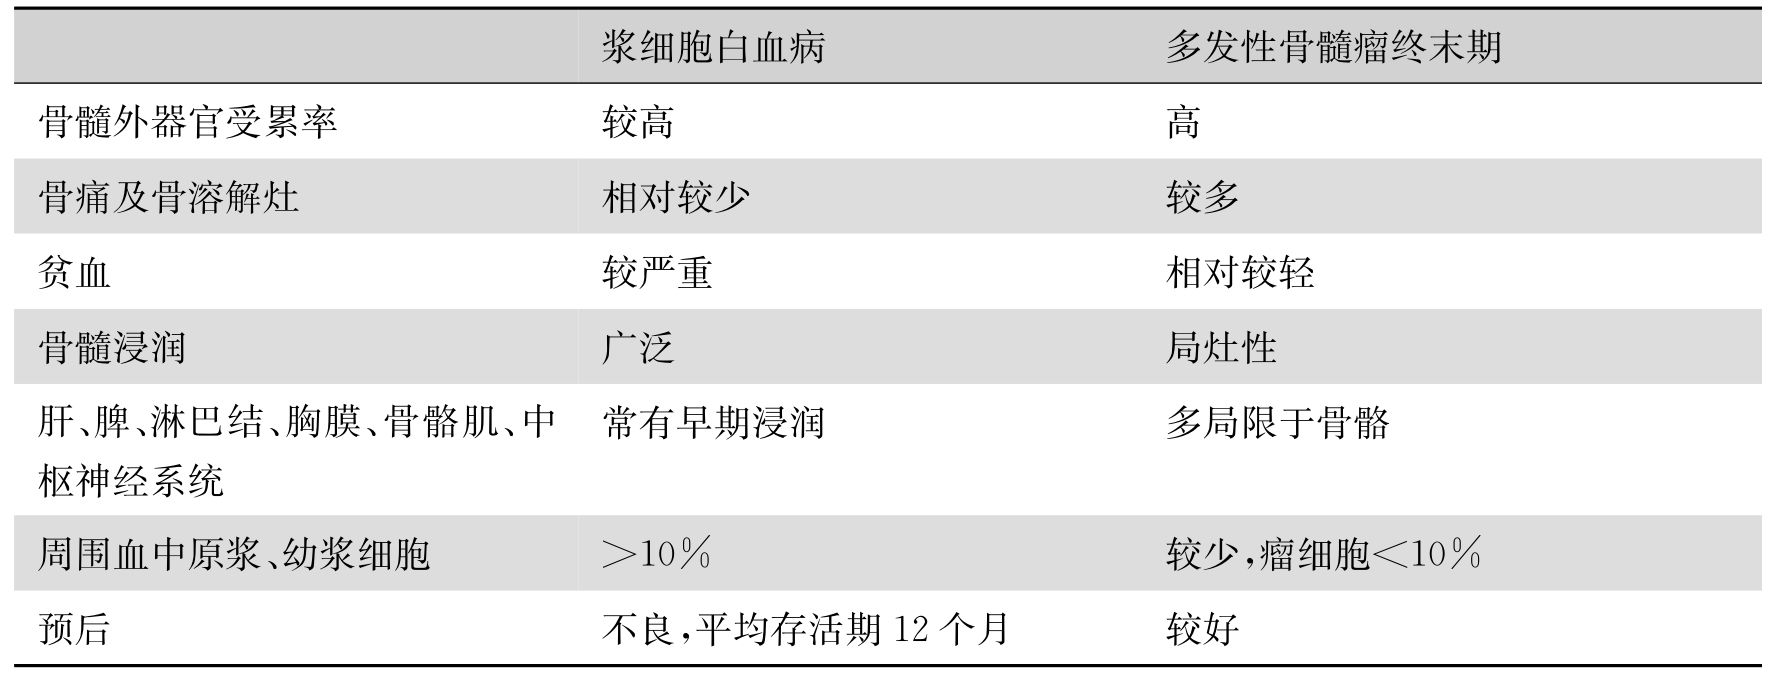
\includegraphics[width=5.90625in,height=2.27083in]{./images/Image00188.jpg}
\end{table}

\paragraph{三、多发性骨髓瘤}

多发性骨髓瘤是恶性浆细胞病中最常见的一种类型,其特征是单克隆的浆细胞恶性增生浸润骨骼和软组织,伴有大量单克隆的免疫球蛋白(M蛋白)的出现和沉积。正常多克隆浆细胞增生和多克隆免疫球蛋白分泌受到抑制,从而引起广泛骨质破坏、反复感染、贫血、高钙血症、高黏滞血症、肾功能不全等一系列临床表现。本病占血液系统恶性肿瘤的10\%,多于50~70岁发病,40岁以下者少见,高峰是55岁。我科统计的资料显示中位发病年龄为53岁。男∶女=3∶1,随着人口老龄化,近十年MM发病率有所上升。

多发性骨髓瘤引起贫血的机制:①瘤细胞增生致红系生长受抑制;②红细胞寿命缩短;③促红细胞生成素减少;④转铁蛋白浓度下降;⑤肾衰竭。本病贫血的诊断标准为Hb低于正常值的20g/L或低于100g/L。

实验室检查:①血清蛋白电泳中出现异常条带,主要在于β、γ球蛋白区域,M蛋白峰表现为以窄底单株峰,而多克隆免疫球蛋白增殖性疾病时表现为宽底高峰(β、γ区大量增殖,两区之间的间隙消失,也称γ-β)。②免疫固定电泳检查发现异常沉淀弧,蛋白质在pH
8.8电泳缓冲液先分离,电泳后的蛋白与相应的5种抗血清γ(IgG)、α(IgA)、μ(IgM)和轻链κ、λ(包括游离、非游离)形成复合物,并被固定在相应的位置上,比血清蛋白电泳更敏感、特异。目的是为鉴别血清蛋白电泳中出现的异常条带或M蛋白量少,以致用血清蛋白电泳方法无法鉴定时。③免疫球蛋白的定量,可发现某一类别(双克隆型有2种)的免疫球蛋白含量增高,同时伴其他类别的免疫球蛋白含量下降。④常规的X线检查可发现弥漫性骨质疏松、穿凿样或虫蚀样溶骨性病变、病理性骨折等改变。⑤骨髓内出现异常浆细胞,比例>15\%。应注意的是,当浆细胞在5\%~10\%时(占MM的5\%),要特别注意浆细胞的形态特点,异常浆细胞(瘤细胞)的特点是:细胞体积较大,圆形或卵圆形,核仁1~2个,核染色质细致,核周淡染区消失,胞浆量丰富,嗜碱性强,可见空泡与少量的嗜苯胺蓝颗粒,若发现成堆明显异常的浆细胞,即可明确诊断。由于骨髓瘤细胞早期常为灶性分布,当诊断有怀疑时,应做多部位特别是疼痛部位的骨髓穿刺(图\ref{fig33-8})。

正常γ球蛋白用免疫电泳法可分成五种:即IgM、IgG、IgA、IgE及IgD。免疫球蛋白分子是对称的,系二条轻链和二条重链由二硫键连接而成。轻链分成二种抗原型:κ型和λ型。五种免疫球蛋白的重链结构则各有不同,分别以μ、γ、α、ε及δ表示。本周蛋白仅由轻链构成。番木瓜酶能将免疫球蛋白分子分成F与S两种碎片。S碎片又称Fab段,由轻链与一部分重链(Fd段)构成。F碎片由重链余下的部分(Fc)及与其连接的碳水化合物所构成。多发性骨髓瘤应与以下疾病相鉴别:

\begin{figure}[!htbp]
 \centering
 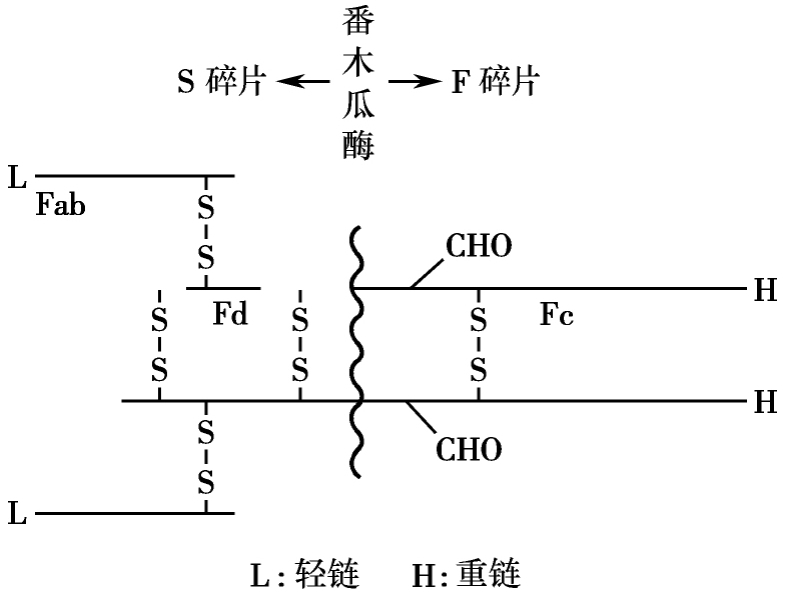
\includegraphics[width=2.66667in,height=1.98958in]{./images/Image00189.jpg}
 \captionsetup{justification=centering}
 \caption{免疫球蛋白分子结构}
 \label{fig33-8}
  \end{figure} 

\subparagraph{1.未定性单克隆丙球蛋白血症(意义未明的单克隆丙球蛋白血症)}

与多发性骨髓瘤鉴别要点有:①未定性单克隆丙球蛋白血症血清中M蛋白一般<30g/L,尿轻链<0.5g/L;②骨髓中浆细胞<10\%;③无贫血,肾功能不全及高钙血症,无溶骨性损害;④β2微球蛋白水平正常。

\subparagraph{2.能产生M蛋白的恶性疾病}

原发性巨球蛋白血症、重链病、慢性淋巴细胞白血病、恶性淋巴瘤(B细胞型)、POEMS综合征、原发性轻链型淀粉样变、Castleman病、髓外浆细胞瘤、孤立性浆细胞瘤、浆细胞性白血病、血管免疫母细胞性T细胞淋巴瘤。

\subparagraph{3.反应性浆细胞增多症------多克隆免疫球蛋白增殖性疾病}

可以引起反应性浆细胞增多的疾病有:恶性肿瘤、慢性感染性疾病、慢性风湿性疾病、肝病、过敏性疾病、再生障碍性贫血等。这些疾病与多发性骨髓瘤的主要鉴别点为:①浆细胞增多有限,骨髓中浆细胞<10\%;②浆细胞分化良好,行流式细胞术检查浆细胞多为非克隆性;③分泌增多的免疫球蛋白多为多克隆性,血清蛋白电泳可见基底部增宽峰或带,免疫固定电泳无M蛋白;④反应性浆细胞增多症本身无临床症状,不需治疗。

\subparagraph{4.骨转移癌、骨结核的溶骨损害}

骨髓转移癌多伴有成骨表现,在溶骨缺损周围有骨密度增加,而且血清碱性磷酸酶常升高。骨痛多在安静时尤其夜间更明显。应详细找寻原发性肿瘤灶。此外在极个别严重全身性骨结核时也可见溶骨损害。

\paragraph{四、系统性肥大细胞增多症}

本病亦称系统性组织肥大细胞病或系统性肥大细胞病,是由于组织肥大细胞异常增殖而引起的一种全身性疾病。主要临床表现有疲倦、乏力、发热、皮肤潮红、皮疹、体重减轻、牙龈出血、恶心呕吐、腹痛、贫血、骨痛以及肝、脾、淋巴结肿大等。病变累及多个器官,无典型临床表现,但皮肤潮红与色素性荨麻疹是本病常有的症状。由于过去对本病认识不足,诊断甚为困难。诊断主要根据骨髓检查中发现大量组织肥大细胞的存在。血与尿液组胺排量增多亦有诊断意义。自1982年上海华山医院报告一例以来(上海医学,5:347,1982),国内又陆续有报道,我科2012年报道3例系统性肥大细胞增多症(中华内科杂志,2012第9期)。原因不明的贫血伴皮肤潮红与慢性皮疹是提供本病诊断的线索。

\paragraph{五、骨髓纤维化}

作骨髓穿刺遇到骨质特别坚硬,且难以获得骨髓成分,提示本病诊断的可能性。同时周围血内有幼稚红细胞和幼稚粒细胞出现,肝脾大尤其是脾大明显,则本病的可能性甚大,骨髓活检常可得到最后的确诊。

骨髓纤维化时,骨髓呈不规则的纤维组织或骨质增生。临床与血液学方面有三项特征:①贫血与进行性脾大;②骨髓活检可见正常骨髓被纤维组织所替代;③周围血中出现众多的幼稚红细胞和幼稚粒细胞。本病并非过于少见。有人将本病分为原发性与继发性。继发性者可继发于结核病、骨髓转移癌、恶性淋巴瘤、白血病和化学物品中毒等。在确定原发性骨髓纤维化前应尽可能除外上述各病的可能性。引起继发性骨髓纤维化的原发病容易从临床表现或特殊检查中获得诊断。偶有原发病不明显,需要多次或多部位的骨髓涂片及活体组织检查,才能确定继发性骨髓纤维化的诊断。原发性骨髓纤维化主要应与慢性粒细胞型白血病相区别(表\ref{tab33-13})。

\begin{table}[htbp]
\centering
\caption{原发性骨髓纤维化与慢性粒细胞型白血病的鉴别}
\label{tab33-13}
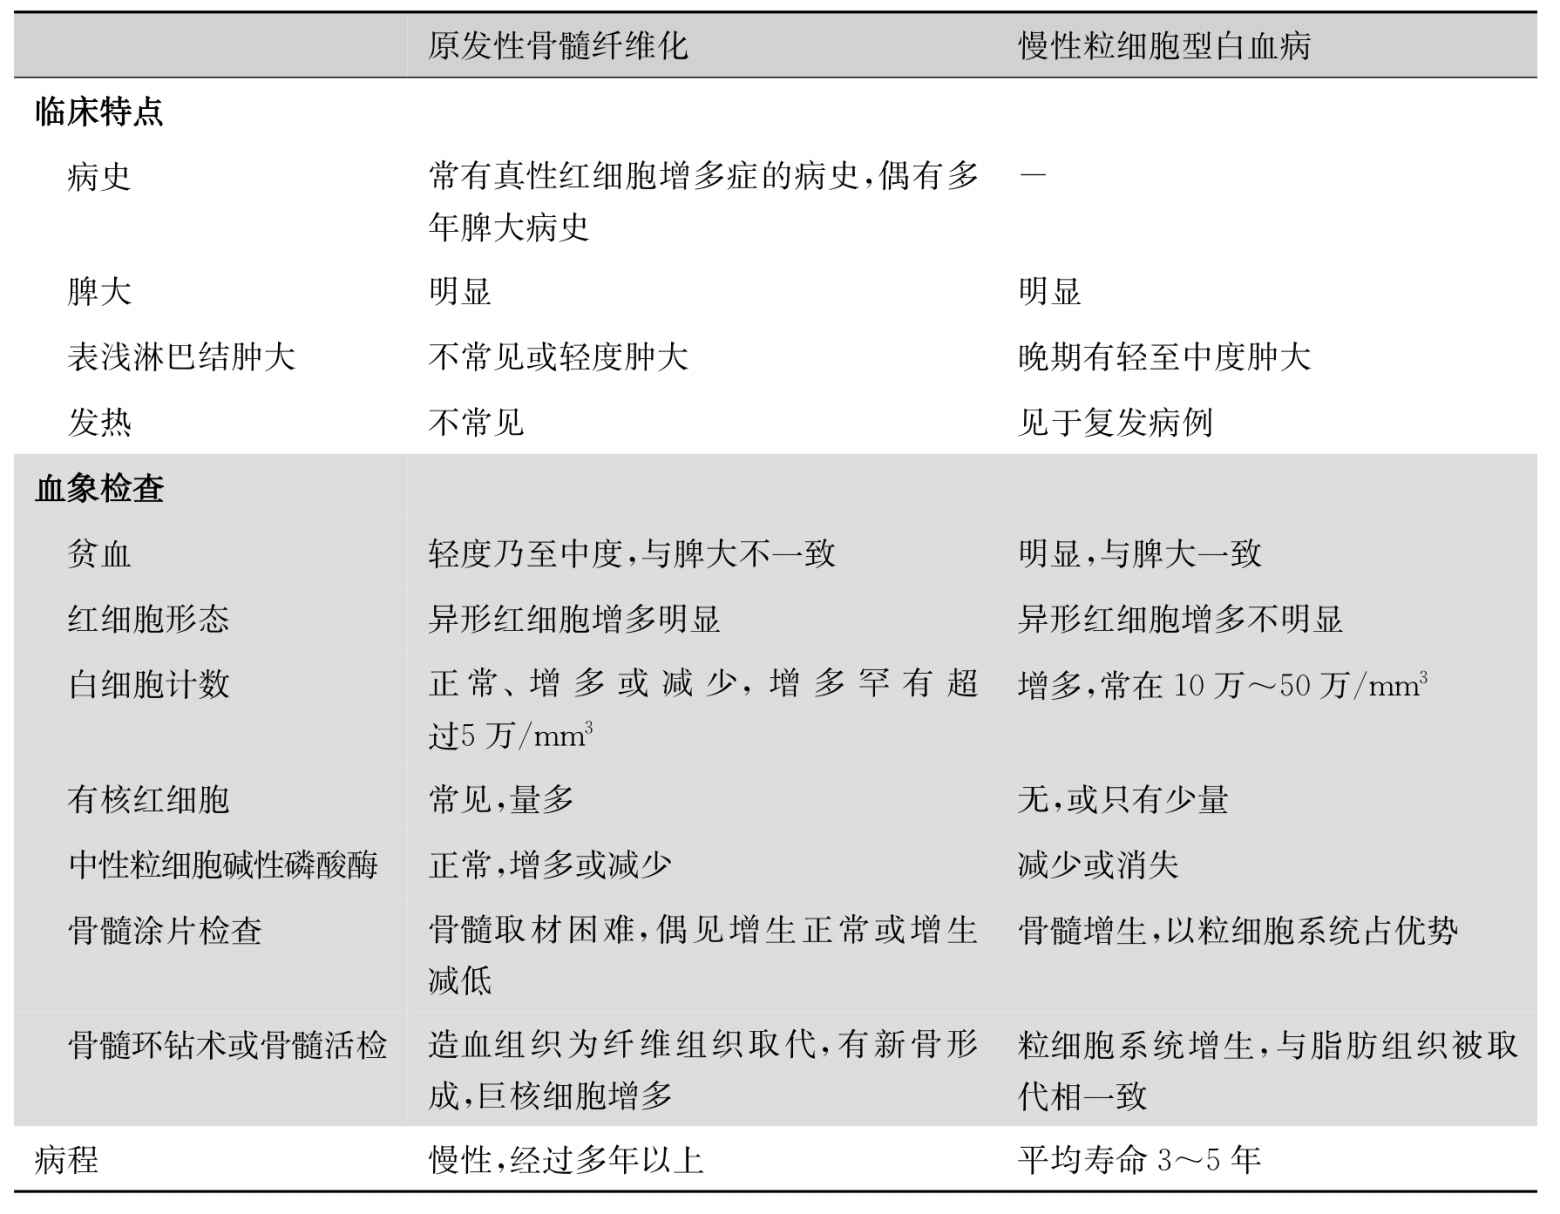
\includegraphics[width=5.95833in,height=4.63542in]{./images/Image00190.jpg}
\end{table}

有人根据放射性铁的研究,帮助本病的诊断,并可作为估计脾脏的造血功能和溶血功能的参考。若脾脏造血和溶血两种功能均旺盛,不宜切脾;若脾脏造血功能不佳而溶血功能旺盛,则切脾是一种合理的治疗方法。

骨髓纤维化与真性红细胞增多症及慢性粒细胞型白血病关系密切,三者可互相转化。

\paragraph{六、大理石骨病(石骨症)}

本病可能是遗传性疾病,较常由放射科作骨照片时发现。石骨症可引起自发性骨折。骨髓管与海绵质均变为致密的骨质。国外文献报道约1/4病例出现骨髓痨性贫血。但据中山医学院报告的四例均无明显的贫血。国内陆续有个案报道本病,患者通常有脾大及呆滞、起皱的面容。

\paragraph{七、再生障碍性贫血}

\subparagraph{(一)再生障碍性贫血}

再生障碍性贫血(再障)是一组由化学物质、生物因素、放射线或不明原因引起的骨髓造血功能衰竭,以造血干细胞损伤、骨髓脂肪化、外周血全血细胞减少为特征的疾病。抗肿瘤药、解热镇痛药、磺胺药、苯化合物、肝炎病毒及放射线是引起再障的中高危因素。其发病机制可能为:造血干/祖细胞内在性缺陷;异常免疫反应损失造血干/祖细胞;造血微环境支持功能缺陷;遗传倾向。其中,机体免疫异常导致造血干/祖细胞损伤被认为是再障最重要的发病机制。

再障的临床表现主要为贫血、出血和感染。临床症状的轻重取决于血红蛋白、白细胞和血小板减少的程度。根据患者的临床表现、血象和骨髓象,可将再障分为急性和慢性两型。两者起病的快慢、严重性以及病变的广泛程度不同,导致完全不同的预后。两者主要鉴别要点见表\ref{tab33-14}。急性再障又称重型再障Ⅰ型,慢性再障在疾病过程中可出现急性再障的表现,称为重型再障Ⅱ型。

\begin{table}[htbp]
\centering
\caption{急性和慢性再生障碍性贫血的鉴别}
\label{tab33-14}
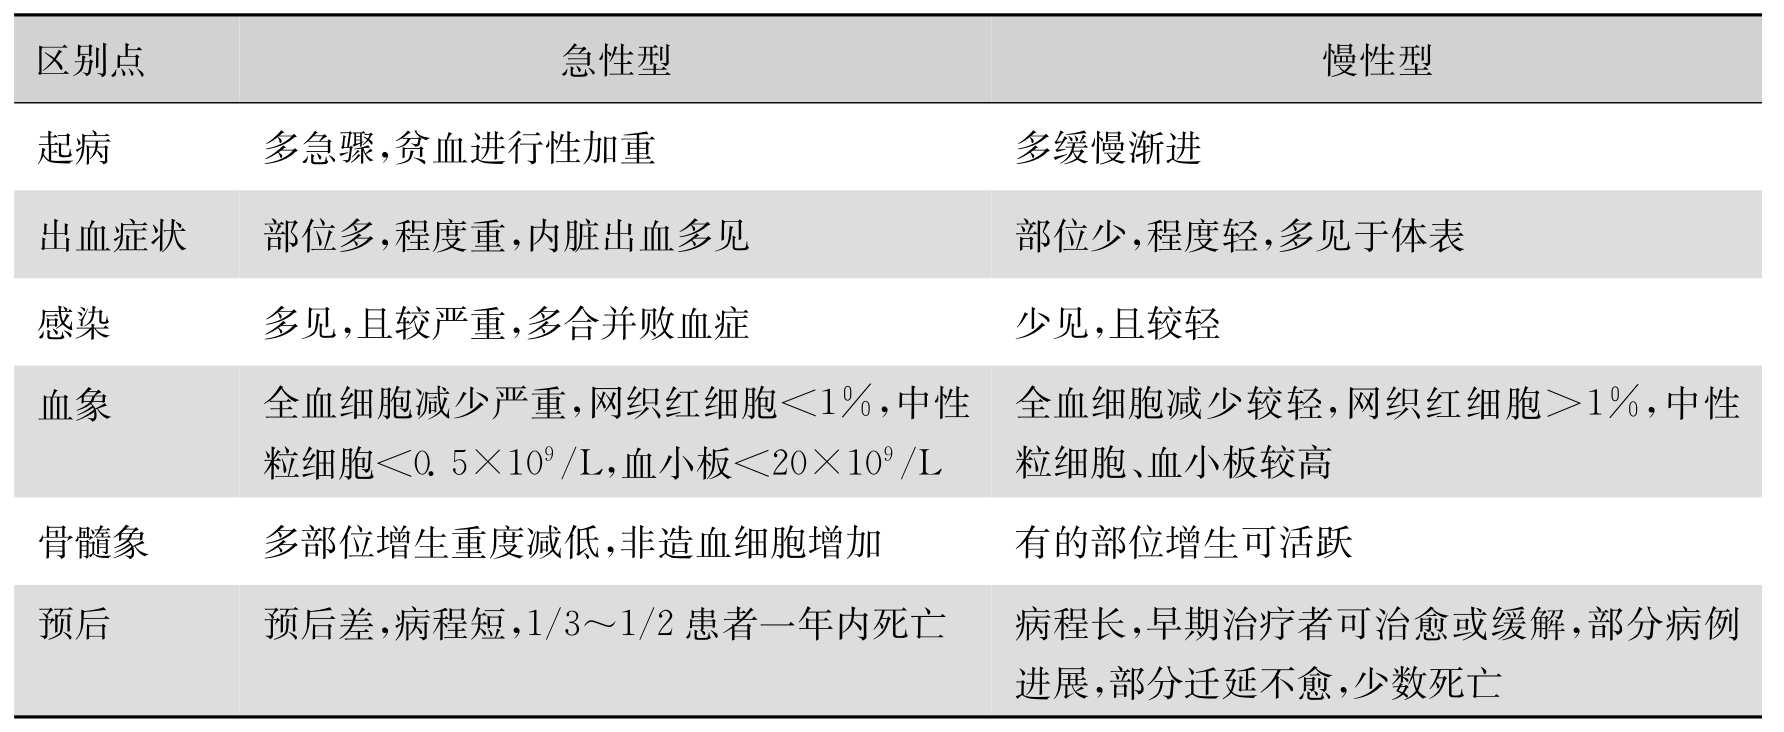
\includegraphics[width=5.9375in,height=2.42708in]{./images/Image00191.jpg}
\end{table}

再生障碍性贫血的诊断根据是:①全血细胞减少(三系细胞减少的先后或程度可以不同);②无明显肝、脾、淋巴结肿大;③血象显示网织红细胞绝对值减少;④骨髓检查显示至少一部位增生不良(包括增生减低或重度减低);如增生良好,须有巨核细胞的减少;⑤能除外其他引起全血细胞减少的疾病(如阵发性睡眠性血红蛋白尿、骨髓增生异常综合征、急性造血功能停滞、轻型地中海贫血、脾功能亢进、急性白血病、骨髓纤维化等)。

再障应着重与以下可引起全血细胞减少的疾病相鉴别:

\hypertarget{text00261.htmlux5cux23CHP33-6-3-4-7-1-1}{}
1.阵发性睡眠性血红蛋白尿

本病的主要表现为慢性贫血,有的病例全血细胞减少,如无血红蛋白尿发作,则与再障易混淆,尤其是有些病例造血功能减低,其骨髓也增生低下,更与再障的骨髓近似。但PNH是造血功能低下并生成带有PNH缺陷的红细胞,其Ham试验、糖水试验、蛇毒因子试验等均阳性。而再障为阴性,可与之鉴别。

\hypertarget{text00261.htmlux5cux23CHP33-6-3-4-7-1-2}{}
2.骨髓增生异常综合征

其中难治性贫血以贫血为主要症状,外周血可呈全血细胞减少,故易与慢性再障相混淆。但前者以病态造血为特征,骨髓象增生明显活跃,尤以红系显著,可见红系、粒系及巨核系病态造血。这些改变不应见于再障。

\hypertarget{text00261.htmlux5cux23CHP33-6-3-4-7-1-3}{}
3.恶性组织细胞病

本病虽全血细胞减少,与再障相似,但患者常伴有非感染性高热,肝、脾、淋巴结肿大,黄疸,多部位骨髓检查可找到异常组织细胞,可与之鉴别。

\hypertarget{text00261.htmlux5cux23CHP33-6-3-4-7-1-4}{}
4.急性白血病

骨髓检查原始细胞明显增多,≥20\%,与再障鉴别一般不难。

\hypertarget{text00261.htmlux5cux23CHP33-6-3-4-7-1-5}{}
5.急性造血功能停滞

常由感染或药物引起,起病快,以高热、贫血、外周全血细胞减少为主要表现,易与再障相混淆。但本病有如下特点可与再障区别:贫血重,网织红细胞可为0,伴粒细胞减少,但血小板减少多不明显,出血轻;骨髓增生多活跃,二系或三系减少,但以红系减少为著,片尾部可见巨大原始红细胞;病情为自限性,不需特殊治疗,2~6周可恢复;血清铜显著增高,红细胞铜减低。

\subparagraph{(二)先天性再生障碍性贫血(Fanconi贫血)}

本病罕见。临床特点:①几乎全发生在儿童,仅偶见于成人;②有家族史;③周围血呈全血细胞减少,骨髓增生极度减低;④部分病例可伴有其他系统发育异常(皮肤色素沉着、睾丸发育不全、骨骼畸形等)。

\subparagraph{(三)纯红细胞再生障碍性贫血(pure red cell aplasia,PRCA)}

是以骨髓单纯红系造血衰竭为特征的一组疾患,其临床特征以贫血为主。外周血红细胞、血红蛋白和网织红细胞减少,骨髓象幼红细胞明显减少或缺如。国内已有不少病例报告。

纯红细胞再生障碍性贫血骨髓象的M/E比值增高。本病又名幼红细胞减少症(erythroblastopenia),包括溶血性贫血再障危象、先天性红细胞增生不良性贫血及获得性红细胞增生不良性贫血三种类型。

\hypertarget{text00261.htmlux5cux23CHP33-6-3-4-7-3-1}{}
1.溶血性贫血再障危象

溶血性贫血患者突然出现贫血加重,此时并非溶血加剧,而是造血障碍。此外,感染和变态反应疾病等非溶血性贫血患者也可出现这种现象。上述疾病出现贫血或原有贫血加剧(白细胞数及血小板数有时也可减少)及网织红细胞有不同程度的减少时,提示红系造血功能的急性停滞。

本病骨髓象特点是:①红细胞系统明显减少,为各细胞系统受阻最突出者;②粒细胞系统相对值虽明显增加,但中性粒细胞呈巨幼样改变,表示该系统发育受阻;③巨核细胞系统明显增加,但多为无血小板形成和退行性变者;④巨型原始血细胞多在涂片的两侧和尾部可找到。

\hypertarget{text00261.htmlux5cux23CHP33-6-3-4-7-3-2}{}
2.先天性红细胞增生不良性贫血(Backfan and Diamond型)

本病患者多系婴儿,发病年龄在6个月以内者占多数,其主要表现为慢性进行性贫血,白细胞及血小板计数正常。骨髓象呈红细胞系统受累,红细胞系统增生减低及成熟阻滞(阻滞于中幼红阶段),分类计数中淋巴细胞略高,粒细胞系统及巨核细胞系统正常。

\hypertarget{text00261.htmlux5cux23CHP33-6-3-4-7-3-3}{}
3.获得性红细胞增生不良性贫血

本病罕见,约1/3病例并存良性胸腺肿瘤;在发病机制上,两者可能有一定的关系。患者的周围血呈正色素性正细胞性贫血,白细胞及血小板数正常。骨髓象特征为:有核红细胞消失或接近消失,而粒细胞系统和巨核细胞系统正常。胸腺切除术后,约30\%PRCA患者无需其他治疗而获得完全缓解(CR)。有的在应用免疫抑制剂后达CR。

\protect\hypertarget{text00262.html}{}{}

\section{参考文献}

1.第八届全国贫血学术会议纪要.中华血液学杂志,1997,18(12):670

2.阮长耿.造血性疾病的分子生物学研究.中华血液学杂志,1996,17(3):115

3.曾溢涛.血红蛋白病的诊断和治疗.中华血液学杂志,1996,17(8):393

4.邵家鸿,等.我国临床血液学研究现况与展望.中华血液学杂志,1995,16(4):171

5.卢新天.遗传性球形红细胞增多症发病机制、诊断及治疗进展.中国小儿血液与肿瘤杂志2009,14(6):243-245

6.任兆瑞,等.遗传性血液病的产前诊断.中华血液学杂志,1991,12(12):660

7.孙佩艳,等.缺铁性贫血研究进展.中华血液学杂志,1996,17(6):327

8.李蓉生.缺铁性贫血的临床研究.中华血液学杂志,1997,18(11):561

9.曾瑞萍,等.α与β地中海贫血双重杂合子基因诊断.中华血液学杂志,1998,19(10):525

10.王沙燕,戴勇.地中海贫血分子诊断的研究进展.中国生育健康杂志,2003,14(3):189

11.邹农.等.76例阵发性睡眠性血红蛋白尿症患者临床特点分析.中华血液学杂志,2012,33(6):471-474

12.张之南,等.阵发性睡眠性血红蛋白尿的临床诊断经验.中华内科杂志,1995,34(8):540

13.高维强.阵发性睡眠性血红蛋白尿症发病机制的研究进展.国外医学·内科学分册,2001,28(11):475-479

14.杜涛,等.阵发性睡眠性血红蛋白尿的研究进展.中华血液学杂志,1997,18(10):557

15.曹琼.新生儿溶血病的产前诊断方法研究进展.中国输血杂志,2003,16(1):67-68

16.张健.Rh血型系统的分子遗传学及其医学应用.中华医学遗传学杂志,2002,19(3):246-249

17.许莹,等.63例自身免疫性溶血性贫血的病因探讨.中华血液学杂志,1996,17(8):428

18.黄振东,等.自身免疫性溶血性贫血免疫病理机制及免疫抑制治疗策略.国际输血及血液学杂志,2012,35
(1):81-84

19.陈琳,等.急性巨核细胞白血病三例.中华内科杂志,1999,38(2):131

20.敖忠芳,徐大为.药物所致急性骨髓衰竭的临床探讨.中华血液学杂志,1992,13(6):299

21.王沁馨.再生障碍性贫血的发病机制与临床治疗的研究进展.国外医学·临床生物化学与检验学分册,2000,21(1):30-32

22.童秀珍,等.系统性肥大细胞增生症三例并文献复习.中华内科杂志,2012,51(9):716-718

23.金洁,等.骨髓增生异常综合征诊断分型标准.中华血液学杂志,2012,33(7):507-508

24.肖志坚.进一步规范我国骨髓增生异常综合征的诊治策略.中华血液学杂志,2012,33(7):505-506

25.张静楠,等.纯红细胞再生障碍性贫血的研究进展.诊断学理论与实践,2010,9(3):280-284

26.李蓉生.慢性病贫血.中华检验医学杂志,2012,34(2):190-192

27.中国多发性骨髓瘤诊治指南(2011年修订).中华内科杂志,2011,50(10):892-896

28.李娟.继发性单克隆免疫球蛋白血症的诊断与治疗.中国实用内科杂志,2007,27(19):1497-1499

\protect\hypertarget{text00263.html}{}{}

